\section{Detección de patologías en pulmones con Rayos X}

Diferentes trabajos se han limitado a clasificar \textit{COVID-2019} y \textit{no COVID-2019} (o
neumonía). Es por ello que, durante este trabajo, desarrollamos un sistema más completo para
distinguir 15 diferentes enfermedades pulmonares.

En este trabajo se desarrolla un método basado en aprendizaje profundo usando una red
\textit{ResNet50} como \textit{backbone}, una red ampliamente usada por la comunidad para implementar
diferentes métodos de análisis de imágenes. Se tomó como base el dataset \textit{ChestX-Ray14} y se
realizó una extensión incluyendo radiografías de pacientes infectados y no infectados por
\textit{COVID-19}. El entrenamiento usando este nuevo dataset consiste en 3 etapas: la primera basada
en \textit{data transfer learning} con la red \textit{ResNet50} preentrenada con el dataset de
ImageNet y reemplazando la capa de clasificación por un nuevo clasificador para las 15 patologías;
una etapa de \textit{fine-tuning} para ajustar las últimas capas convolucionales; y una última etapa
de \textit{full-tuning} para ajustar completamente los pesos de la red. Los experimentos completados
muestran que esta propuesta es capaz de preservar el rendimiento de los clasificadores entrenados
para las 14 patologías previas del estado del arte y, al mismo tiempo, alcanzar el rendimiento de los
clasificadores binarios para \textit{COVID-19} mostrados en la literatura actual. Adicionalmente, se
demuestra que el modelo y entrenamiento propuesto puede ser usado para realizar fácilmente una
extensión hacia alguna otra patología, con la implementación de un clasificador binario para la
detección de Tuberculosis, una particular neumonía bacteriana \cite{stirenko2018chest}, con
rendimiento comparable con diversos métodos de deep learning \emph{ad hoc} \cite{puttagunta2021detection}.


La evaluación del modelo propuesto para el diagnóstico de las 15 patologías demuestra la obtención de
resultados competitivos, en particular para \textit{COVID-19}. Se realiza la comparación del modelo
con trabajos recientes que clasifican las primeras 14 patologías (excluyendo \textit{COVID-19}). Los
resultados en términos del \textit{Área Bajo la Curva del Operador del Receptor de Características - AUC}
muestran un rendimiento competitivo contra el método propuesto para detección de patologías
\textit{ChestX-Ray14} y un notable rendimiento en la detección de neumonía para \textit{COVID-19}.

\section{Materiales y Métodos}
En la ejecución de este trabajo se usa la base de datos \textit{ChestX} \cite{wang2017chestx} y se
incluyen imágenes de Rayos-X para \textit{COVID-19} y \textit{saludables} (imágenes de personas sin
alguna enfermedad de pulmón identificada). El dataset \textit{ChestX-ray14} contiene 112,120
radiografías de tórax de vista frontal (\textit{frontal-view}) \textit{AP} y \textit{PA}
(anterior-posterior y posterior-anterior) de 30,805 pacientes únicos. Cada imagen está anotada con
algunas de las etiquetas correspondientes a las 14 patologías descritas previamente. Este dataset es
enriquecido previamente al proceso de entrenamiento descrito aquí con radiografías de personas con
neumonía y \textit{saludables}. La tabla \ref{table_dataset} resume la composición del dataset
completo usado en este trabajo.


\begin{table}[!ht]
    \centering
    \begin{tabular}{| r |l | c | c | c |}
     \hline
     Class & Disease & Source & Train & Test  \\
     \hline\hline
     1  & Cardiomegaly       & 1 & 5897  & 1069 \\
     2  & Emphysema          & 1 & 3496  & 1093 \\
     3  & Effusion           & 1 & 13737 & 4658 \\
     4  & Hernia             & 1 & 4470  & 86   \\
     5  & Infiltration       & 1 & 17122 & 6112 \\
     6  & Mass               & 1 & 7862  & 1748 \\
     7  & Nodule             & 1 & 9250  & 1623 \\
     8  & Atelectasis        & 1 & 13762 & 3279 \\
     9  & Pneumothorax       & 1 & 6303  & 2665 \\
     10 & Pleural-Thick.     & 1 & 8022  & 1143 \\
     11 & Pneumonia          & 1 & 6031  & 555  \\
     12 & Fibrosis           & 1 & 9072  & 435  \\
     13 & Edema              & 1 & 6953  & 925  \\
     14 & Consolidation      & 1 & 9796  & 1815 \\
     ---&  Healthy           & 1 & 35645 & 9861 \\
     \hline
     11 & Pneumonia          & 2 & 5475  & 594  \\
     15 & COVID-19           & 2 & 2873  & 1904 \\
     ---&  Healthy           & 2 & 8661  & 1926 \\
     \hline
    \end{tabular}
    \caption{Número de radiografías de pecho por patología en el conjunto de datos. Fuentes (DS): (1) ChestX-ray14,
             (2) Compilación de bases de datos de internet. Pleural-Thick. es una abreviación para Pleural-Thickening.}
    \label{table_dataset}
\end{table}

\subsubsection{Re-etiquetamiento de datos}
\label{ssec_relabelling}

Para lograr un entrenamiento del modelo exitoso, se usa la versión re-etiquetada de la base de
\textit{ChestX-ray14} propuesta por los autores de \textit{CheXNet} \cite{rajpurkar2018deep}. De
acuerdo con \cite{rajpurkar2018deep}, los datos re-etiquetados permiten mejorar el proceso de
entrenamiento significativamente. Cada re-etiquetado se realiza a través del entrenamiento de
múltiples modelos de redes neuronales con los datos originales como entrada. Los modelos con mejor
precisión en la evaluación del dataset original son conservados. Después, las predicciones
individuales de cada modelo son promediadas y se construye un detector binario para cada patología
usando un umbral que permita maximizar la métrica F1-score en todas las patologías (véase la sección
\ref{sec_metrics} para la definición de F1-score). Finalmente, cada dato es re-etiquetado como
positivo si este fue originalmente etiquetado como positivo o si el clasificador construido en el
paso previo resulta positivo.

A pesar de este re-etiquetado, en estos experimentos los datos preservan su estructura de acuerdo
con los datos de entrenamiento y validación proporcionados originalmente. Para el conjunto de datos
originales, solo se usan los datos de entrenamiento re-etiquetados, es decir, solo se usan los datos
con etiquetas modificadas en la etapa de entrenamiento, preservando la evaluación intacta al proceso
usado por otros métodos. Aun así, se muestra el reporte correspondiente al conjunto de validación
re-etiquetado solo como referencia adjunto en el Apéndice.


\subsubsection{Procesamiento de los datos}

El procesamiento de las imágenes radiográficas sigue un camino simple: se realiza un redimensionamiento a
$1024 \times 1024$ y $384 \times 384$ píxeles para cada modelo como es descrito en la siguiente sección. Dicho
redimensionamiento se realiza mediante la interpolación basada en área; calculando el valor del píxel en la imagen de
salida como el promedio de los píxeles que cubren la región correspondiente en la imagen de entrada. Este enfoque es
especialmente útil para evitar artefactos y conservar la calidad de la imagen cuando se reduce su tamaño.
Posteriormente, sigue un proceso de ecualización por histograma a cada imagen resultante, con la intención de mejorar
el contraste de esta misma. La idea es distribuir los valores de intensidad de los píxeles de manera más uniforme en la
imagen. La ecualización por histograma se realiza en el canal de luminancia de la imagen (Y), ya que es el canal que
contiene la información de brillo de la imagen.
El canal de luminancia se extrae de la imagen original en el espacio de color YUV y se equaliza. Finalmente, la imagen
se reconstruye combinando el canal de luminancia ecualizado con los canales de crominancia originales.

Como paso final del preprocesamiento de los datos, se realizó una normalización a la imágen usando los valores de
media y desviación estándar del conjunto
de datos de \text{ImageNet}. Básicamente, se ajustan los valores de los píxeles de la imagen para que tengan una
distribución más uniforme y características similares a las imágenes de usadas para el modelo pre-entrenado.
Cabe mencionar que cuando se aplica la ecualización de histograma al canal Y del espacio YUV, se ajusta el contraste de
la imagen, mejorando la distribución de los niveles de brillo. Este paso realza detalles en la imagen, haciendo que las
áreas oscuras sean más claras y viceversa. Después de esta ecualización, cuando se normaliza la imagen, la normalización
se aplicará sobre los valores ajustados. La normalización tiene como objetivo ajustar los valores de los píxeles a un
rango específico basado en la media y la desviación estándar de la base de datos original del modelo preentrado
(\textit{ImageNet}), pero no anula la ecualización de histograma aplicada previamente; es decir, ambos pasos son
complementarios: la ecualización de histograma mejora la distribución del brillo y la normalización ajusta los valores
de los píxeles para ser más adecuados para el modelo de aprendizaje automático. De los resultados observables de este
proceso y como se ve en las imágenes de las secciones siguientes, no generaron artefactos en las dichas imágenes y al
contrario su objetivo es mejorar su calidad y proceso de entrenamiento.

Los datos de entrada al modelo neuronal basado en \textit{ResNet50} son imágenes de 1024 columnas y 1024 filas con 3
canales idénticos y de 384 columnas y 384 filas con 3 canales idénticos para el modelo basado en \textit{ViT}.
La principal decisión de la diferencia entre los tamaños de entrada de las imágenes radica en la arquitectura de la red
neuronal y el costo en consumo de memoria de cada una limitada por la infraestrucura computacional usada.
La red \textit{ResNet50} es una red convolucional profunda caracterizada por su capacidad de captar características
espaciales locales mediante convoluciones. Por otro lado, la red \textit{ViT} es una red basada en transformers que
captura relaciones a largo plazo y patrones globales en la imagen a través de la atención. Bajo esta premisa, creemos
que la red de \textit{ViT} funciona bien con imágenes de menor tamaño, ya que los transformers no dependen tanto de las
convoluciones locales como las redes convolucionales.

Finalmente, siguiendo la propuesta de \textit{CheXNet}, se hace uso de múltiples funciones de pérdida tipo
\textit{Binary Cross-Entropy} con distintos pesos para solventar el desbalanceamiento de clases.


\begin{equation} \label{eq:loss}
    L(\hat y, y) = \sum_{c=0}^{15} \left[ w_c^{(p)} y_c \log \hat y_c + w_c^{(n)} (1-y_c) \log (1- \hat y_c) \right],
\end{equation}

\noindent donde $y$ es el vector de etiquetas reales, $\hat{y}$ es el vector de etiquetas predichas,
$w_c^{(p)}$ y $w_c^{(n)}$ son los pesos para los casos positivos y negativos de cada clase $c$,
respectivamente. Dichos pesos son calculados como sigue:

\begin{equation}\label{eq:weights}
    w_c^{(n)} = \frac{n_c}{N} \;\;\;\; \text{and} \;\;\;\; w_c^{(p)} = 1-  w_c^{(n)};
\end{equation}

\noindent donde $N$ es el tamaño del conjunto de datos, y $n_c$ el número de imágenes radiográficas con
etiquetas $c$ (el número de elementos del vector de la $c$-ésima clase iguales a 1). Nótese que los
pesos son inversamente proporcionales al número de casos en la clase.


\section{Arquitecturas usadas}

\subsection{CNN y Transfer Learning}

El modelo desarrollado se construye tomando \textit{CheXNet} como referencia \cite{rajpurkar2018deep},
el cual clasifica entre 14 enfermedades usando el conjunto de datos \textit{ChestX-Ray14}
\cite{wang2017chestx}. El modelo propuesto se construye desde cero y extiende la propuesta de
\textit{CheXNet} para incluir la clasificación de imágenes con \textit{COVID-19}.

\textit{CheXNet} es un modelo basado en redes neuronales para detectar la presencia de 14 diferentes
enfermedades de pulmón. \textit{CheXNet} usa imágenes de Rayos X de vista frontal como entrada y un
modelo convolucional preentrenado como backbone \cite{rajpurkar2018deep}. El modelo backbone usado
por \textit{CheXNet} es la red \textit{DenseNet121} \cite{huang2017densely}, que contiene 121 capas
convolucionales entrenadas con la base de datos de \textit{ImageNet} \cite{ILSVRC15}. Las imágenes
analizadas por el modelo pueden corresponder a vistas anterior-posterior o posterior-anterior. La
implementación de Transferencia de Conocimiento se logra removiendo la etapa de clasificación
(formada por capas densas) mientras que la etapa convolucional previa permanece intacta, funcionando
como un extractor de características. Posteriormente, se coloca una nueva etapa de clasificación
construida para la detección de 14 enfermedades en su lugar. Finalmente, la nueva red compuesta se
entrena usando la base de datos \textit{ChestX-Ray14}, manteniendo fijos los pesos correspondientes
a la etapa convolucional de la red.

Así como en \textit{CheXNet}, un modelo usado como backbone y entrenado con la base de datos de
\textit{ImageNet} define la red entrenada para detectar patologías torácicas. Motivados por
\citeauthor{bressem2020comparing, shazia2021comparative}, quienes muestran que una red backbone en
particular no es un elemento definitivo en el rendimiento de detección del modelo, sino el proceso
de entrenamiento. Adicionalmente, \citeauthor{huang2017densely, luo2020comparison} presentan
comparaciones de modelos evaluados en la clasificación de ImageNet donde \textit{ResNet50} y
\textit{DenseNet201} obtienen un accuracy de $76\%$ y $74\%$ respectivamente. Por ello, se realiza
la elección del modelo \textit{ResNet50} como backbone en la implementación de la red convolucional.
\textit{ResNet50} fue propuesta por \citeauthor{he2016deep} y es una opción popular en la
implementación de sistemas de reconocimiento generales, dada su eficiencia computacional y
relativa sencillez de entrenamiento (por su grafo de gradientes con pocos caminos) en comparación
con el candidato natural \textit{DenseNet121} usado en \textit{CheXNet}, cuyas versiones alternativas
del modelo \textit{CheXNet} están disponibles en \cite{chexnet_code}. A pesar de lo anterior, no se
descarta el uso e investigación en un futuro de otros modelos como backbone, ya sea inclusive
\textit{DenseNet} o \textit{efficientNet} \cite{tan2019efficientnet}. Sabiendo que este mismo
procedimiento puede guiarnos a incluir nuevas patologías tales como Tuberculosis Pulmonar
\cite{stirenko2018chest}; un tipo de neumonía bacteriana mayormente común en países en vías de
desarrollo y también frecuentemente reportado en pacientes con síndrome de inmunodeficiencia
adquirida (AIDS) \cite{matsuura2018tuberculous}.


En la red detectora, la etapa clasificadora del modelo \textit{ResNet50} es reemplazada con dos capas
densas y una operación de \textit{Dropout} intermedia con una probabilidad del $25\%$. La tabla
\ref{table_resnet50} resume la arquitectura de la red.

\begin{table}[!ht]
    \centering
    \begin{tabular}{| l|c | c | r |}
    \hline
                 &     Input   &  Output    &  \\
    Layer        &   dimension & dimension  & Parameters \\
    \hline\hline
    ResNet50     &     3,1024,1024 &     2048,1,1 & 24,036,431 \\
    Flatten      &     2048        &     2048     &  --        \\
    Dense        &     2048        &     256      & 524,544    \\
    ReLU         &     256         &     256      & --         \\
    Drop-0.25  &     256         &     256      & --         \\
    Dense        &     256         &     15       &  3,855     \\
    Sigmoid      &     15          &     15       & --         \\
    \hline
    \end{tabular}
    \caption{Arquitectura de la red neuronal usada en el modelo propuesto basado en ResNet50. Las capas
    densas incluyen el término de bias. \textit{Drop-0.25} significa una capa \textit{Dropout} con
    probabilidad de 0.25.}
    \label{table_resnet50}
\end{table}

\subsection{Vision Transformers}

Los modelos \textit{Vision Transformers} (\textit{ViT}) \cite{DBLP:journals/corr/abs-2010-11929},
propuestos en el año 2020, son una variante de los modelos Transformer diseñados para resolver tareas
de visión por computadora. En lugar de utilizar convoluciones, como tradicionalmente se haría con
otros modelos para extraer las distintas características de la imagen, los modelos Vision Transformers
descomponen la imagen de entrada en una serie de parches, a los que posteriormente se les asigna un
token y se aplica la arquitectura de Transformer estándar presentada anteriormente, véase la figura
\ref{fig_ViT}.


\begin{figure}[htp]
    \centering
    {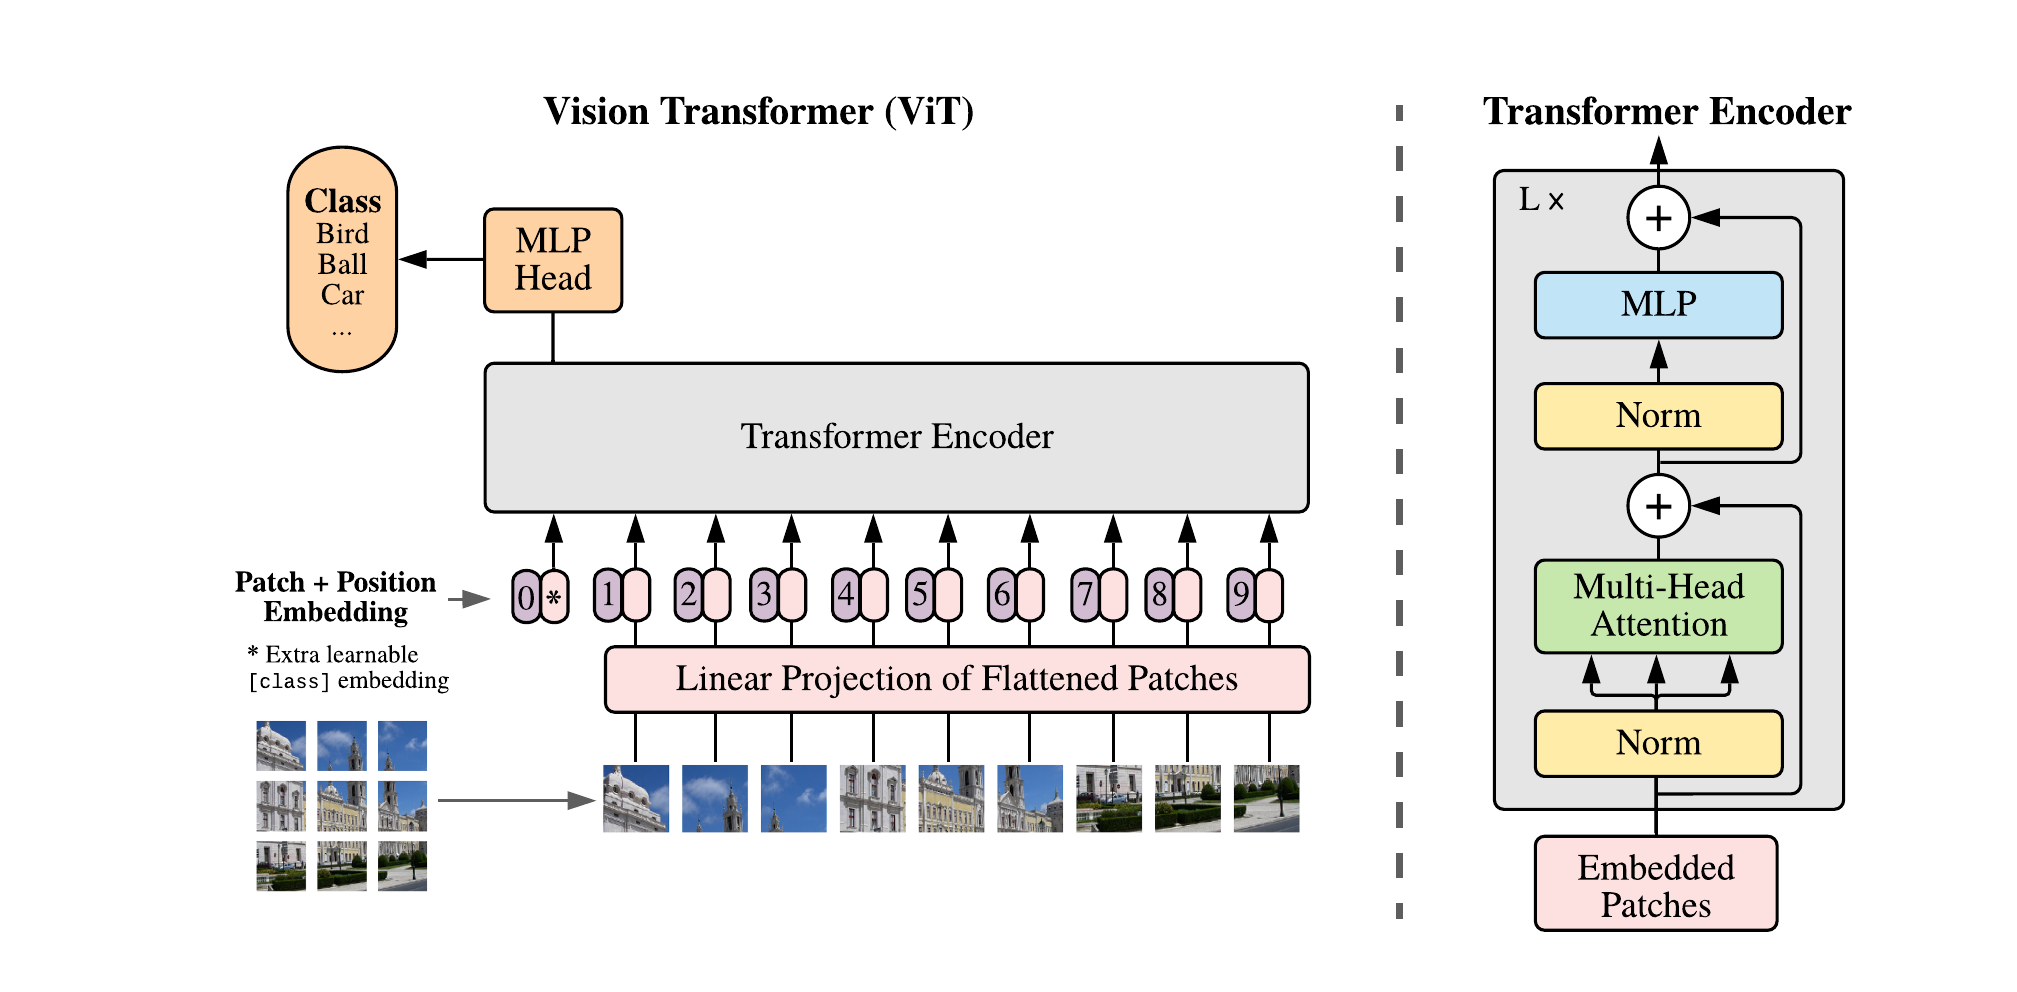
\includegraphics[width=1.0\textwidth]{Chapters/4. ViT-Lung/images/ViT.png}}
\caption{Representación original del modelo ViT mostrado en \cite{DBLP:journals/corr/abs-2010-11929}.
Las imágenes a procesarse son descompuestas en una serie de parches (3x3 parches en este ejemplo). Los
parches generados son proyectados a una dimension linear agregándose información posicional.}
\label{fig_ViT}
\end{figure}

El mecanismo de atención en el modelo ViT transforma continuamente los vectores de representación de
los parches de la imagen, incorporando relaciones semánticas entre ellos. Análogamente a como se usa
en el área de Procesamiento de Lenguaje Natural, mientras los vectores avanzan en profundidad en el
modelo Transformer, las relaciones semánticas formadas entre los parches se vuelven más complejas.
Esto reemplaza las características extraídas a través de operaciones convolucionales. Para realizar
estas tareas, el modelo ViT solo utiliza la parte codificadora de la arquitectura general del Transformer,
codificando y extrayendo la información relevante de las imágenes en las etapas de multi-atención.

A pesar de que los enfoques dirigidos con modelos ViT y CNN son diferentes, algunas investigaciones
indican que la representación de la información en capas inferiores es bastante similar, es decir,
convoluciones más internas que guardan características locales y cabezas de atención más profundas
\cite{DBLP:journals/corr/abs-2108-08810}. Aun así, los modelos ViT incorporan más información global
que los modelos CNN en capas inferiores y los \textit{skip connections} influyen más en los modelos
ViT que en los basados en CNN. Además, como describen en su artículo \citeauthor{DBLP:journals/corr/abs-2010-11929},
los modelos ViT se benefician de entrenamientos con conjuntos de datos mucho más grandes en comparación
con los datos necesarios para obtener resultados favorables en CNN.

Basados en las propuestas de \citeauthor{DBLP:journals/corr/abs-2010-11929}, la red clasificadora
implementada se deriva de los modelos entrenados que describen. Los modelos se entrenan utilizando
varios conjuntos de datos: el conjunto de datos ILSVRC-2012 de ImageNet, que consta de 1k clases y
1.3 millones de imágenes; el conjunto de datos ImageNet-21k, que contiene 21k clases y 14 millones
de imágenes; y el conjunto de datos JFT, que incluye 18k clases y 303 millones de imágenes de alta
resolución. Estos conjuntos de datos proporcionan una amplia variedad de ejemplos que permiten al
modelo aprender y generalizar eficazmente.


\begin{table}[!ht]
    \centering
    \begin{tabular}{| l | c |}
     \hline
    \textbf{Input size}  & 384 $\times$ 384 \\
    \textbf{Patch size}  & 32 $\times$ 32 \\
    \textbf{Layers}      & 12  \\
    \textbf{Hidden size} & 768 \\
    \textbf{MLP Size}    & 3072 \\
    \textbf{Heads}       & 12 \\
    \textbf{Params}      & 87M \\
     \hline
    \end{tabular}
    \caption{Configuración de la arquitectura del modelo ViT usado. Usa imágenes de tamaño
             $384 \times 384$ con 3 canales correspondientes al modo RGB. En total cuenta con 12
             cabezas de atención y 12 codificadores internos.}
\label{table_ViTBase}
\end{table}

La arquitectura del modelo ViT está basada en las implementaciones de los Transformers
mostrados en \textit{BERT} \cite{DBLP:journals/corr/abs-1810-04805}. Presentan distintas nomenclaturas
para definir el tamaño del modelo generado. En particular, se ha usado en este trabajo la arquitectura
\textit{ViT-Base-patch32-384}. \quotes{Base} hace referencia al modelo base de \textit{BERT},
\quotes{patch32} a la variante que trabaja con parches de tamaño $32 \times 32$ y \quotes{384} a las
dimensiones de las imágenes de entrada al modelo. En la tabla \ref{table_ViTBase} y \ref{table_ViT}
se ejemplifica la arquitectura mencionada; 12 capas codificadoras del Transformer conforman el modelo
ViT, con 12 cabezas de atención con un tamaño de 768 y, finalmente, las componentes MLP de tamaño 3072.

En la red detectora basada en ViT, la etapa clasificadora del modelo \textit{ResNet50} también es
reemplazada con dos capas densas y una operación de \textit{Dropout} intermedia con una probabilidad
del $25\%$, similar al modelo de CNN propuesto anteriormente.


\begin{table}[!ht]
    \centering
    \begin{tabular}{| l|c | c | r |}
    \hline
                 &     Input   &  Output    &  \\
    Layer        &   dimension & dimension  & Parameters \\
    \hline\hline
    ViT     &     3,384,384 &     768 & 87,416,064 \\
    Dense        &     768        &     256      & 196,864    \\
    ReLU         &     256         &     256      & --         \\
    Drop-0.25  &     256         &     256      & --         \\
    Dense        &     256         &     15       &  3,855     \\
    Sigmoid      &     15          &     15       & --         \\
    \hline
    \end{tabular}
    \caption{Arquitectura ViT usada en el modelo propuesto. Las capas densas incluyen el término de bias.
    Drop-0.25 significa una capa de Dropout con una probabilidad de 0.25.}
    \label{table_ViT}
\end{table}

\begin{figure}[htp]
    \centering
    {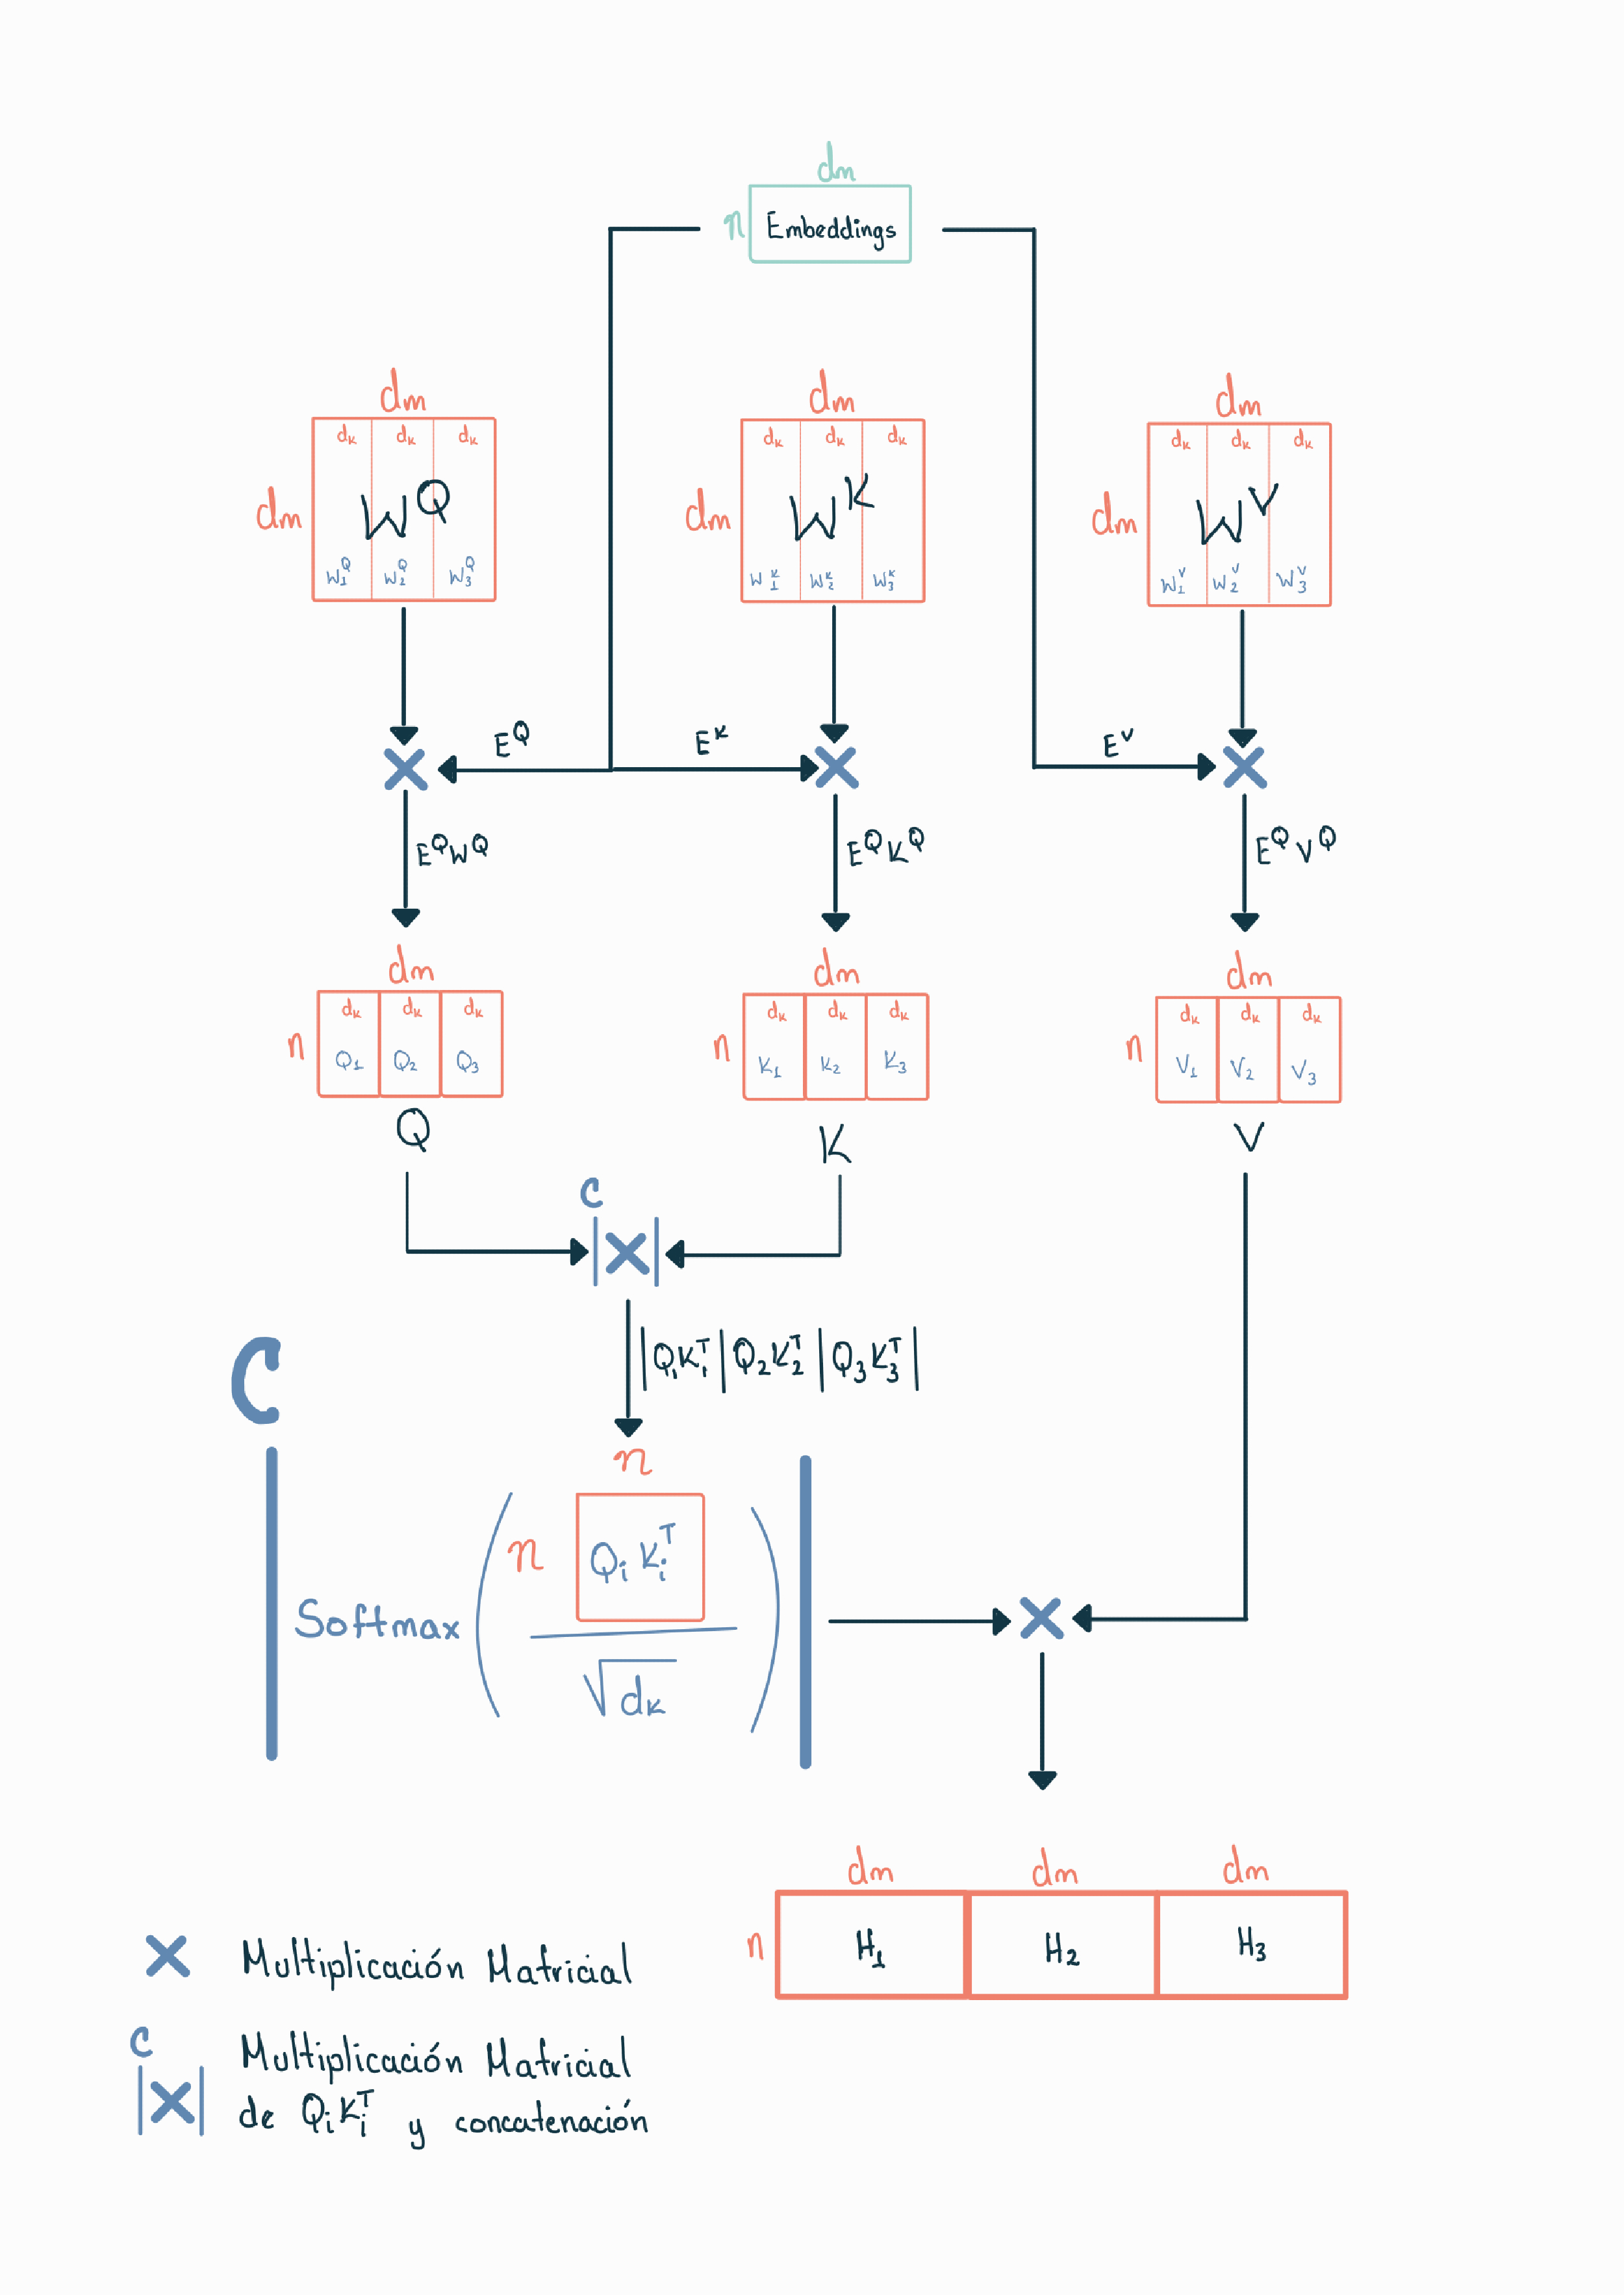
\includegraphics[width=0.7\textwidth]{Chapters/4. ViT-Lung/images/cabezas_vit.jpg}}
\caption{Representación gráfica del módulo de MultiHead Self-Attention en el modelo ViT usando 3 cabezas
         de atención. Se observa
         que el tamaño de la matriz de atención $Q_i K_i^T$ es dependiente del número de parches
         generados en la imagen al igual que el tamaño de cada cabeza de atención $H_i$ depende de
         la dimensión de estos. Las cabezas de atención resultantes finalmente son re-proyectadas
         a dimensiones $n \times d_m$ para las etapas posteriores. }
\label{vit-head-dim}
\end{figure}


\begin{figure}[htp]
    \centering
    {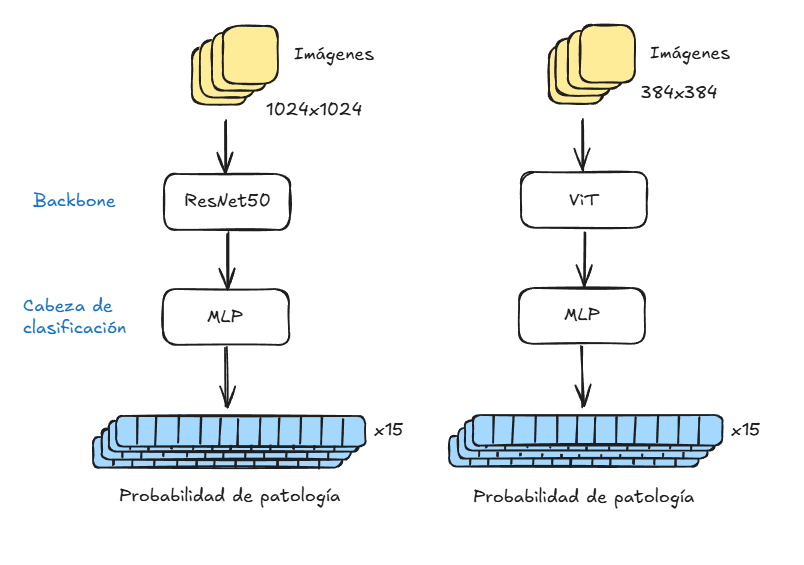
\includegraphics[width=0.5\textwidth]{Chapters/4. ViT-Lung/images/both_models.png}}
\caption{Esquema de los modelo basado en ResNet50 y Vit para la detección de las 15 patologías pulmonares.}
\label{net_both}
\end{figure}


% \subsection{ViT con cabezas de atención Flexibles}

% Como se observó en la sección \ref*{section-mha} el Transformer está basado en la idea de
% Multihead-Self-Attention, permitiendo al modelo conjuntamente atender a información en diferentes
% posiciones desde distintos subespacios de representación

% \begin{equation}
%     mha(Q, K, V) = Concat(head_1,head_2,head_3,..., head_h)W^O
% \end{equation}

% con $E_Q, E_K, E_V \in \mathbb{R}^{n \times d_{m}}$ como embeddings de entrada, $n$ es el tamaño de la
% secuencia, $d_m$ es el tamaño del embedding y $h$ el número de cabezas de atención. Cada cabeza de
% atención está indicada como:

% \begin{equation}
%     head_i = Attention(E_Q W_i^Q, E_K W_i^K, E_V W_i^V) =
%     Sofmax\Big(\frac{E_Q W_i^Q (E_K W_i^K)^T}{\sqrt{d_k}}\Big) E_V W_i^V
%     \label{eq:head-mha}
% \end{equation}

% donde $W_i^Q$, $W_i^K$ $\in \mathbb{R}^{d_m \times d_k}$, $W_i^V$ $\in \mathbb{R}^{d_m \times d_v}$,
% $W^O$ $\in \mathbb{R}^{hd_v \times d_m}$ y $d_k=d_v=d_m/h$.

% Observando la ecuación \label{eq:mha} podemos identificar algunas propiedades que se cumplen en el
% modelo de Transformes

% \begin{itemize}
%     \item El tamaño de la cabeza es dependiente de la dimensión del embedding y el número de cabezas
%           de atención.
%     \item Mientras más cabezas de atención los embeddings son proyectados a dimensiones de subespacios
%           de representación cada vez menores, indicando una mayor compresión de la información en estos.
%     \item La necesidad de escalar el modelo implica escalar conjuntamente todas las dimensiones.
% \end{itemize}

% Con ello en mente la hipótesis es que la redefinición de $W_i^Q$, $W_i^K$, $W_i^V$ $\in \mathbb{R}^{d_m \times d_h}$,
% $W^O$ $\in \mathbb{R}^{hd_h \times d_m}$ con $d_h$ como un hiperparámetro y $d_h > d_k$
% podemos tener mayor control de las cabezas de atención y sobre la representación
% del aprendizaje de cada una de ellas.

\subsection{Proceso de Entrenamiento}
\label{ss:archiecture}

% \subsubsection{Proceso de entranamiento para el modelo CNN}

% we present the procedure to train our models to detect the 15 pathology's (including COVID-19) from a network pre-trained with ImageNet.
\begin{enumerate}
    \item \textbf{Entrenamiento inicial}.\\
        \textbf{Modelo CNN}: Una vez seleccionada la red convolucional pre-entrenada con la base de datos de
        ImageNet, se reemplaza la etapa de clasificación por una nueva compuesta por dos capas densas. En la
        tabla \ref{table_resnet50} se presentan los detalles de la red \textit{ResNet50} usada en este modelo.
        De esta forma, la red convolucional \textit{ResNet50} funciona como un extractor de características;
        transforma los datos originales (las imágenes de radiografías) en una nueva representación que contiene
        las características que permiten distinguir entre las distintas patologías. El clasificador se implementa
        agregando dos capas densas a esta red base. En la etapa de entrenamiento, la red se comporta como una red
        Perceptrón Multicapa (\textit{Multilayer Perceptron}, MLP) donde la entrada es el tensor de características
        calculado por la red base o backbone. Para entrenar el clasificador, los pesos que corresponden a la red
        base son congelados y solamente se actualizan los pesos que pertenecen a la etapa de clasificación (las
        capas densas descritas en la tabla \ref{table_resnet50}). El entrenamiento se realiza durante 35 épocas,
        conservando el mejor modelo de acuerdo al \textit{accuracy} obtenido usando el conjunto de validación.

        \textbf{Modelo ViT}: Al igual que el modelo CNN, con la red basada en Transformers y pre-entrenada con la
        base de datos ILSVRC-2012 de ImageNet, se reemplaza la etapa de clasificación por la misma red compuesta
        por dos capas densas. En la tabla \ref{table_ViTBase} y \ref{table_ViT} se presentan los detalles de la
        arquitectura de la red \textit{ViT}. Similar al modelo convolucional, el modelo \textit{ViT} trabaja
        extrayendo características y encontrando relaciones a través de la atención. Esto le permite determinar
        características esenciales para poder identificar las distintas patologías trabajadas. El clasificador
        añadido a la red contiene dos capas densas que procesan la información del modelo ViT y determinan
        finalmente la clasificación correspondiente para cada dato. Durante la primera etapa de entrenamiento,
        los pesos entrenables asociados al modelo \textit{ViT} que conforma la red son congelados, permitiendo
        solo el entrenamiento del modelo clasificador. El entrenamiento se realiza durante 25 épocas,
        conservando el mejor modelo de acuerdo al valor de \textit{accuracy} obtenido usando el conjunto de
        validación.


    \item \textbf{Fine-tuning}\\
        \textbf{Modelo CNN}: Hasta este punto, el enfoque usado es un \textit{aprendizaje superficial} y la
        etapa de extracción de características está completamente desasociada de la etapa de clasificación. La
        ventaja de implementar el sistema a través de dos redes neuronales (la red backbone y la red MLP) es que
        podemos mejorar la extracción de características en términos de la tarea de interés. Para ello, se procede
        a descongelar las últimas capas convolucionales de la red backbone y continuar el entrenamiento en conjunto
        con las capas densas de la etapa clasificadora. Las capas a descongelar corresponden al último bloque
        construido de la 5° etapa convolucional (\textit{layer conv5\_3}) \cite{he2016deep}. Así, permitimos que el
        tensor obtenido a la salida de la red backbone sea particularizado a la tarea de clasificación actual. El
        procedimiento de \textit{Fine-tuning} es realizado por 20 épocas más.\\

        \textbf{Modelo ViT}: Siguiendo un procedimiento similar al modelo propuesto basado en \textit{ResNet50}, se
        procede a descongelar los dos últimos bloques del modelo ViT, esto es, los correspondientes a los bloques 11
        y 12 de acuerdo a la arquitectura vista en la tabla \ref{table_ViT}. Esto permite, de manera similar, que las
        salidas del modelo ViT sean más particulares a la tarea de clasificación en cuestión. 12 épocas más de
        entrenamiento le siguen a este modelo.


    \item \textbf{Full-tuning}\\
        \textbf{Modelo CNN}: Las razones por las cuales solamente son reentrenadas las últimas capas
        convolucionales son que tenemos que lidiar con el problema del desvanecimiento del gradiente y el sistema
        completo puede terminar sobreajustando sus parámetros a la base de datos de entrenamiento. El primer
        problema no es tan relevante en este punto, el rendimiento obtenido por el modelo es satisfactorio y si no
        fuese posible mejorar los parámetros de las capas convolucionales, tampoco sufren un deterioro. El segundo
        problema es de importancia si la muestra de imágenes radiográficas es suficientemente representativa de las
        patologías de interés, puesto que el sistema es suficientemente general para predecir el conjunto de imágenes
        de prueba correctamente. En este trabajo consideramos que tenemos suficientes datos y, por lo tanto, como
        etapa final del entrenamiento se realiza una afinación completa del modelo. Esto es, entrenando completamente
        la red, la etapa de extracción de características (backbone) y la etapa de clasificación (MLP). Para evitar
        el \textit{over-fitting}, el entrenamiento es continuado solamente por 10 épocas, conservando el mejor modelo
        de acuerdo al \textit{accuracy} obtenido en el conjunto de validación.\\

        \textbf{Modelo ViT}: De acuerdo a la premisa anterior, el modelo \textit{ViT} es descongelado completamente,
        permitiendo el entrenamiento de todos los bloques de la red. Esto permite al modelo especializarse en la
        tarea de detección de patologías pulmonares al ajustar sus pesos por algunas épocas más. De la misma manera,
        el modelo \textit{ViT} es entrenado por 8 épocas más. A diferencia del modelo basado en \textit{ResNet50}, el
        número de épocas es menor en cada etapa para el modelo \textit{ViT} puesto que se observó una convergencia
        más rápida.


\end{enumerate}

Similar a \citeauthor{rajpurkar2018deep}, al inicio de cada etapa de entrenamiento en ambas redes,
las imágenes de entrenamiento son volteadas horizontalmente con 0.5 de probabilidad como técnica de
aumento de datos.

La salida de la red basada en \textit{ResNet50} y \textit{ViT} es un vector de tamaño igual al número
de patologías detectadas, 15. Cada elemento del vector $\tilde y_i \in [0,1]$ puede ser interpretado
como la probabilidad de que la i-ésima patología esté presente en la imagen analizada. El vector
$\tilde y$ no necesariamente tiene que sumar 1, puesto que varias patologías pueden estar presentes
en la radiografía. Una patología es detectada como positiva si $\tilde y > \theta$, donde $\theta$ es
el umbral. El valor típico para este umbral es de $0.5$ y puede ser modificado dependiendo del análisis
de la curva del \textit{Receiver Operator Characteristic}, o \textit{Curva ROC}. Como algoritmo de
entrenamiento se usa \emph{Adam} \cite{kingma2017adam} con un factor de aprendizaje (LR) de
$1\times 10^{-4}$ para el modelo basado en \textit{ResNet50} y $1\times 10^{-5}$ para el modelo basado
en \textit{ViT}, con parámetros de inercia $\beta_1=0.9$ y $\beta_2=0.999$ en ambos modelos y con un
decaimiento (LR-decay) de $0.1$ si después de 10 iteraciones no se detecta una reducción en el valor
de la función de pérdida mayor a $1\times 10^{-4}$ (plateau escape).


\subsubsection{Transfer Learning para la detección de Neumonía por Tuberculosis}

El propósito de esta sección es demostrar que el \textit{backbone} del modelo propuesto basado en
\textit{ResNet50} y entrenado con las 15 patologías mencionadas anteriormente, puede ser la base para
desarrollar detectores para otras enfermedades de pulmón. La idea en esta etapa es no repetir el proceso
completo de entrenamiento, sino usar una simple estrategia de \textit{Transfer Learning}. Así, se procede
a extender el modelo para detectar (junto con las otras enfermedades) neumonía causada por Tuberculosis
\cite{stirenko2018chest}, un tipo de neumonía bacteriana común en países en vías de desarrollo y también
frecuentemente reportada en pacientes con síndrome de inmunodeficiencia adquirida (AIDS)
\cite{matsuura2018tuberculous}.


\begin{table}[!ht]
    \centering
    \begin{tabular}{| r |l | c | c | c |}
     \hline
     Class & Disease & Source & Train & Test  \\
     \hline\hline
     16  & Tuberculosis        & 3 & 888   & 488  \\
     ---&  Non-Tuberculosis     & 3 & 6000  & 1600 \\
     \hline
    \end{tabular}
    \caption{ Número de radiografías de tórax de pacientes con y sin Tuberculosis.}
\label{table_dataset_tb}
\end{table}

El dataset considerado incluye casos de \textit{Tuberculosis} y \textit{no Tuberculosis}, pero es
importante aclarar que la condición en particular de los casos de \textit{no Tuberculosis} no está
especificada por completo, es decir, incluyen tanto pacientes saludables como pacientes con otras
afecciones.

La base de datos (indicada proveniente de la fuente 3 en la tabla \ref{table_dataset_tb}) está
compuesta por radiografías provenientes de: TBX11K dataset \cite{liu2020rethinking}, India (DA and DB)
dataset \cite{chauhan2014role}, Montgomery County dataset \cite{jaeger2014two}, y Shenzhen Hospital
dataset \cite{jaeger2014two}. En este trabajo se usan las listas originales para el entrenamiento y
evaluación definidos para este dataset.


\begin{table}[!ht]
    \centering
    \begin{tabular}{| l| c | c | r |}
     \hline
                 &  Input       & Output           &   \\
    Layer        &  dimension    & dimension        & Parameters \\
    \hline\hline
    Initial Backbone & & & \\ \hline
    ResNet50     &  3,1000,1000 &     2048,1,1     & 24,036,431 \\
    Flatten      &     2048     &     2048         &  --        \\
    Dense        &     2048     &     256          & 524,544    \\
    ReLU         &     256      &     256          & --         \\
    Drop-0.25    &     256      &     256          & --         \\
    \hline
    Additional Branch & & & \\ \hline
    Dense$^\ast$ &     256      &     128          &  38,896     \\
    ReLU         &     128      &     128          & --         \\
    Drop-0.20    &     128      &     128          & --         \\
    Dense$^\ast$ &     128      &      1           &  129       \\
    Sigmoid      &      1       &      1           & --         \\
     \hline
    \end{tabular}
    \caption{ Arquitectura del modelo de la red de aprendizaje profundo usada en el modelo extendido
             con una rama para Tuberculosis. Las capas densas incluyen el término de bias y $^\ast$
             indica las capas que son entrenables.}
\label{table_resnet50_tb}
\end{table}

Para poder detectar Tuberculosis, se realiza la implementación de un clasificador binario usando como
\textit{backbone} la red \textit{ResNet50} entrenada previamente para la detección de las 15 patologías
anteriores. La nueva rama de clasificación incluye dos nuevas capas densas (con sus respectivas funciones
de activación). Conservamos los parámetros correspondientes al \textit{backbone} no entrenables y solo se
entrenan las nuevas capas densas usando la estrategia mencionada en la subsección de {\bf Entrenamiento
Inicial} \ref{ss:archiecture} con el optimizador, factor de aprendizaje y otros parámetros sin cambios y
\textit{Weighted Binary Cross-Entropy} como función de pérdida similar a \eqref{eq:loss}. Este modelo
extendido aún detecta las 15 enfermedades comentadas previamente con una salida binaria extra para
Tuberculosis. La arquitectura extendida, incluyendo la nueva rama, está descrita en la tabla
\ref{table_resnet50_tb}.


\begin{figure}[htp]
    \centering
    {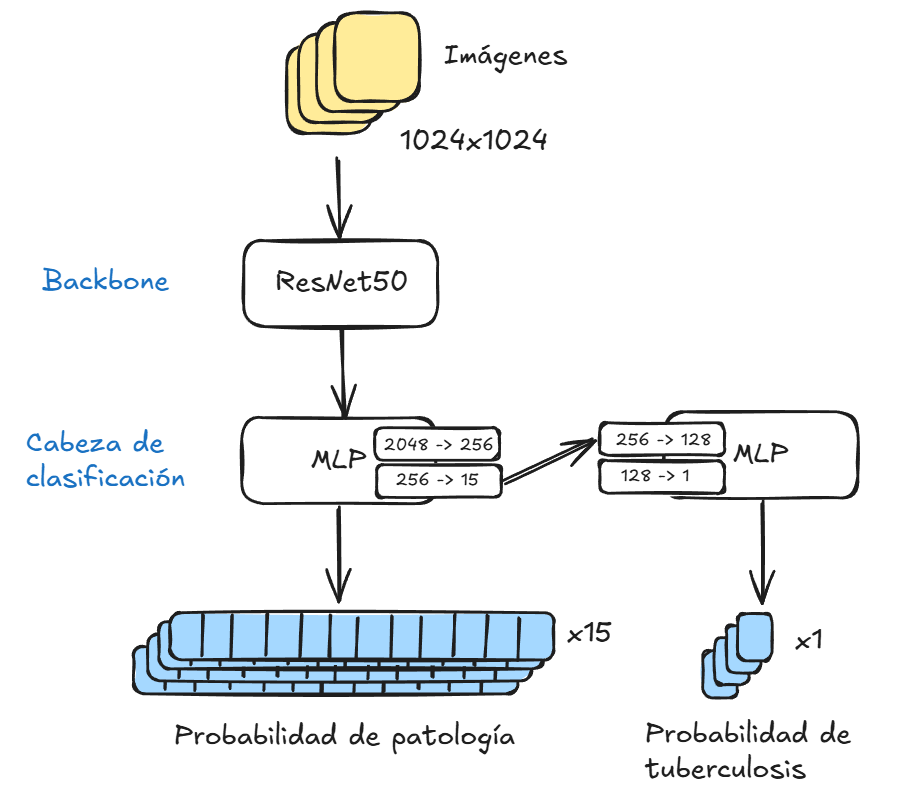
\includegraphics[width=0.5\textwidth]{Chapters/4. ViT-Lung/images/tb_net.png}}
\caption{ Esquema de la extensión del detector de las 15 patologías incluyendo una nueva rama para
          la detección de Tuberculosis.}
\label{net_tb}
\end{figure}


\subsection{Métricas de Evaluación} \label{sec_metrics}

Considerando un problema de clasificación binario donde cada radiografía tiene una etiqueta
$y = \{1, 0\}$ con $1$ indicando la presencia del padecimiento en el paciente y $0$ significando
que se encuentra sano, los detectores pueden tener dos posibles resultados: una detección positiva (P)
para la enfermedad o una detección negativa (N). La tabla \ref{table_cm} muestra la caracterización
de la etiqueta predicha de acuerdo a los valores reales (\textit{Ground Truth}, GT). Si un paciente
enfermo es correctamente detectado, tenemos un \textit{Verdadero Positivo} (\textit{True Positive}, TP)
y si la predicción falla, es un \textit{Falso Negativo} (\textit{False Negative}, FN). Por otro lado,
si una etiqueta positiva es erróneamente predicha en un paciente saludable, entonces tenemos un
\textit{Falso Positivo} (\textit{False Positive}, FP), y si el paciente saludable es correctamente
predicho, es un \textit{Verdadero Negativo} (\textit{True Negative}, TN). La tabla \ref{table_cm}
muestra la \textit{Matriz de Confusión} con el conteo de cada tipo de predicción en el conjunto de
prueba.


\begin{table*}[!ht]
    \centering
    \begin{tabular}{ccccl}
    %\cline{3-4}
    &  & \multicolumn{2}{ c }{Predicción} \\
    %\cline{3-4}
    \multicolumn{1}{c}{}& & Positivo & Negativo &    \\
    \cline{3-4}
    \multicolumn{1}{c}{\multirow{6}{*}{GT} } &
    \\
    \multicolumn{1}{c}{} & Enfermo & TP & FN   &  $ \longrightarrow  R = \frac{TP}{TP+FN}$  \\
    \\
    \cline{3-4}
    \multicolumn{1}{ c }{}                    &
    \\
    \multicolumn{1}{c}{} & No-Enfermo & FP & TN   &  $ \longrightarrow S = \frac{TN}{FP+TN}$   \\
    \\
    \cline{3-4}
    \\
    & & $\downarrow$ & $\downarrow$ & \\
    \multicolumn{1}{c}{} &       & $P = \frac{TP}{TP+FP}$  & $NPV = \frac{TN}{FN+TN}$ &
    \end{tabular}
    \caption{Interpretación de los resultados (predicción) de acuerdo al los valores reales (Ground
             Truth, GT). Las métricas son calculadas como la relación entre el elemento de la diagonal
             y la suma correspondiente por fila o por columna. Según sea el caso: R, \textit{recall}
             o \textit{sensitivity}; S, \textit{specificity}; P, \textit{precision}; NPV,
             \textit{negative prediction value}.}
    \label{table_cm}
\end{table*}

Para este trabajo, asumimos que una patología en particular es correctamente detectada si su
correspondiente puntuación en el vector predicho es más significativa que cierto umbral. En particular,
asumimos un umbral igual para todas las patologías de $0.5$ en ambos modelos. Usando la Matriz de
Confusión podemos definir varias métricas de rendimiento.


\begin{enumerate}
    \item Accuracy ($A$). Esta métrica es quizás la más obvia. Corresponde al razón de los datos
          predichos correctamente sobre el total.
    \begin{equation}
        \label{eq:accuracy}
        A = \frac{TP+TN}{TP+TN+FP+FN}.
    \end{equation}

    \item Recall o Sensibility ($R$). Es la fracción de pacientes con enfermedades correctamente
          detectados. Esta métrica también es conocida como Tasa de Verdaderos Positivos (True
          Positive Rate, TPR), la tasa de detecciones correctas.
    \begin{equation}
        \label{eq:TPR}
        R = \frac{TP}{TP + FN}
    \end{equation}

    \item Specificity ($S$). Es la fracción de pacientes sin enfermedades que son detectados
          correctamente.
    \begin{equation}
        \label{eq:Specificity}
        S = \frac{TN}{TN + FP}
    \end{equation}

    \item False Positive Rate ($FPR$). La tasa de detecciones falsas de enfermedades, es calculada
          como:
    \begin{equation}
        \label{eq:FPR}
        FPR = 1 - S,
    \end{equation}
    donde $S$ es el valor de Specificity.

    \item Precision ($P$). Es la fracción de predicciones positivas que realmente tiene una una
          enfermedad.
    \begin{equation}
        \label{eq:P}
        P = \frac{TP}{TP + FP}
    \end{equation}

    \item $F_1$ Score ($F_1$).  Durante la creación de los modelos buscamos un balance entre Precision y
        Recall. El incremento de alguna de estas dos métricas es en compensación de la otra. Un modelo que predice
        la mayoría de los datos como positivos tendrá un \textit{Recall} más cercano a 1, pues el conteo de
        \textit{Falsos Negativos} será mucho menor, pero los \textit{Falsos Positivos} incrementarán, reduciendo
        la \textit{Precision} del modelo. En caso contrario, si el modelo predice la mayoría de los datos como
        negativos, el conteo de \textit{Falsos Positivos} será menor, incrementando la métrica de \textit{Precision},
        pero los \textit{Falsos Negativos} incrementan, provocando que el \textit{Recall} decremente. El
        \textit{F1-Score} busca un balance entre las dos métricas (\textit{Precision-Recall Trade-Off}). Un
        desequilibrio entre ellas indica un sesgo en cualquiera de las dos maneras descritas anteriormente. Por
        ello, es más informativo como medida de rendimiento usar una media geométrica entre las dos métricas.

    \begin{equation}
        \label{eq:f1}
        F_1 = \frac{2\; P \, R}{P + R}.
    \end{equation}

    \item  Area Under Curve of Receiver Operator Characteristic (AUC-ROC). La Curva Característica
        Operativa del Receptor es un gráfico que muestra las capacidades de diagnóstico de clasificadores
        binarios. Como se mencionó anteriormente, una patología es detectada como positiva si su puntaje
        predicho es más significativo que un umbral dado. Así, ajustando dicho umbral a valores más bajos,
        se permite en general incrementar el TPR, aunque el FPR también puede ser incrementado. La Curva ROC
        resulta de graficar los valores de TPR contra FPR variando el umbral en el intervalo $[0,1]$. El AUC
        corresponde al área bajo la Curva de ROC.


\end{enumerate}


\subsection{Resultados}

La Tabla~\ref{table:res-model-covid} y \ref{table:vit-model-covid} muestra un resumen del rendimiento
de los modelos propuestos. Las imágenes que conforman los conjuntos de entrenamiento, validación y prueba
corresponden a los definidos originalmente en el dataset. En \textit{ChestX-ray14}, se redefinen las etiquetas
de entrenamiento de acuerdo a \textit{CheXNet} \cite{rajpurkar2018deep}; excepto para las imágenes de
\textit{COVID-19} y sin patologías identificadas. Es válido usar cualquier modificación de etiquetas en la
etapa de entrenamiento siempre y cuando se mantenga el conjunto de datos de prueba sin cambios (imágenes de
radiografía y sus etiquetas).

Los resultados presentes se ajustan al procedimiento de entrenamiento y prueba antes descrito para ambos
modelos. Las métricas que se incluyen son: \textit{Area Under the Precision Recovery Curve} (AUC-PR),
\textit{Area Under the Receiver Operating Characteristic Curve} (AUC-ROC), \textit{F1-Score} y
\textit{Accuracy} (Acc.). \textit{Global-14} muestra el rendimiento en las patologías de \textit{ChestX-ray-14}
(clasificaciones correctas vs clasificaciones incorrectas), \textit{Global-15} muestra incluyendo
\textit{COVID-19}. Nótese que los modelos propuestos tienen su mejor rendimiento en la detección de
\textit{COVID-19}, la enfermedad anexada. También se han incluido datos de clases sin patologías detectadas
(\textit{healthy}) debido a la importancia de tener un buen desempeño en la detección de sujetos saludables.
El rendimiento global sobre los datos de \textit{ChestX-ray14} y \textit{COVID-19} se muestra en el último
renglón de la tabla \ref{table:res-model-covid} y \ref{table:vit-model-covid}.


\begin{table*}[tb]
    \centering
    \begin{tabular}{|l||c|c|c|c|}
        \hline
    {\bf Patología} 	    	&	\multicolumn{4}{c|}{\bf Modelo propuesto ResNet50}  \\
    \cline{2-5}
                        &	AUC-PR	&	AUC-ROC 	& F1-Score  & Acc.  \\
        \hline \hline
        Cardiomegaly	&	0.290	&	0.875	&	0.324	&	0.911	\\
        Emphysema	    &	0.413	&	0.938	&	0.350	&	0.886	\\
        Effusion	    &	0.494	&	0.850	&	0.527	&	0.807	\\
        Hernia	        &	0.050	&	0.855	&	0.051	&	0.957	\\
        Infiltration	&	0.382	&	0.740	&	0.458	&	0.711	\\
        Mass	        &	0.290	&	0.831	&	0.340	&	0.877	\\
        Nodule	        &	0.249	&	0.806	&	0.299	&	0.876	\\
        Atelectasis	    &	0.336	&	0.794	&	0.387	&	0.815	\\
        Pneumothorax	&	0.447	&	0.906	&	0.496	&	0.852	\\
        Pleural-Thick	&	0.157	&	0.820	&	0.217	&	0.852	\\
        Pneumonia	    &	0.425	&	0.863	&	0.274	&	0.856	\\
        Fibrosis	    &	0.106	&	0.852	&	0.154	&	0.910	\\
        Edema	        &	0.187	&	0.879	&	0.193	&	0.788	\\
        Consolidation	&	0.150	&	0.776	&	0.234	&	0.754	\\
        \hline
        COVID-19	    &	0.844	&	0.991	&	0.799	&	0.969	\\
        Healthy	        &	0.691	&	0.736	&	0.496	&	0.712	\\
        \hline\hline
        Global-14	    &	0.284	&	0.842	&	0.307	&	0.847	\\
        Global-15	    &	0.321	&	0.852	&	0.340	&	0.855	\\
    \hline
    \end{tabular}
    \caption{Resumen del rendimiento del modelo propuesto basado en \textit{ResNet50}.
            Los conjuntos de datos de validación corresponden a como originalmente
            están definidos en ChestX-ray14. Los etiquetas de entrenamiento corresponden a las
            definidas de acuerdo al re-etiquetado realizado por CheXNet; véase \cite{rajpurkar2018deep}
            El valor de umbral está definido igual a 0.5. Ninguna otra optimización fue realizada.}
    \label{table:res-model-covid}
\end{table*}

\begin{table*}[tb]
    \centering
    \begin{tabular}{|l||c|c|c|c|}
        \hline
    {\bf Patología} 	    	&	\multicolumn{4}{c|}{\bf Modelo propuesto ViT}  \\
    \cline{2-5}
                        &	AUC-PR	&	AUC-ROC 	& F1-Score  & Acc.  \\
        \hline \hline
        Cardiomegaly	&	0.253	&	0.866	&	0.324	&	0.928	\\
        Emphysema	    &	0.246	&	0.866	&	0.319	&	0.924	\\
        Effusion	    &	0.401	&	0.791	&	0.434	&	0.807	\\
        Hernia	        &	0.036	&	0.843	&	0.064	&	0.971	\\
        Infiltration	&	0.256	&	0.621	&	0.235	&	0.724	\\
        Mass	        &	0.227	&	0.768	&	0.296	&	0.900	\\
        Nodule	        &	0.157	&	0.704	&	0.209	&	0.908	\\
        Atelectasis	    &	0.271	&	0.734	&	0.325	&	0.840	\\
        Pneumothorax	&	0.359	&	0.842	&	0.430	&	0.880	\\
        Pleural-Thick	&	0.125	&	0.765	&	0.197	&	0.881	\\
        Pneumonia	    &	0.104	&	0.738	&	0.144	&	0.732	\\
        Fibrosis	    &	0.070	&	0.810	&	0.134	&	0.932	\\
        Edema	        &	0.120	&	0.828	&	0.180	&	0.877	\\
        Consolidation	&	0.118	&	0.715	&	0.171	&	0.836	\\
        \hline
        COVID-19	    &	0.859	&	0.982	&	0.801	&	0.973	\\
        Healthy	        &	0.634	&	0.705	&	0.537	&	0.703	\\
        \hline\hline
        Global-14	    &	0.196	&	0.778	&	0.247	&	0.867	\\
        Global-15	    &	0.240	&	0.791	&	0.284	&	0.874	\\
    \hline
    \end{tabular}
    \caption{Resumen del rendimiento del modelo propuesto basado en \textit{ViT}.
            Los conjuntos de datos de validación corresponden a como originalmente
            están definidos en ChestX-ray14. Los etiquetas de entrenamiento corresponden a las
            definidas de acuerdo al re-etiquetado realizado por CheXNet; véase \cite{rajpurkar2018deep}
            El valor de umbral está definido igual a 0.5. Ninguna otra optimización fue realizada.}
    \label{table:vit-model-covid}
\end{table*}

Es importante recalcar que no es apropiado usar \textit{Accuracy} como único criterio de rendimiento
bajo este contexto. El \textit{Accuracy} de cada clase es calculado como el número de clasificaciones
correctas (TP y TN) entre la suma total de radiografías analizadas. Con clases desbalanceadas, tales
como las que analizamos ahora (patología vs no patología), un modelo podría ser engañoso en cuanto a
su eficiencia, sesgando su clasificación sobre la o las clases más representativas. Si el desbalance
es grande, el modelo puede asignar todos los datos como la clase que representa mayor peso y, por tanto,
tener un buen rendimiento en la métrica de \textit{Accuracy}. A pesar de ello, los datos presentados
son resultados que sirven como referencia para el lector. Una manera más apropiada de medir el desempeño
del modelo es calcular la gráfica de TPR vs FPR para obtener el área bajo la curva, en otras palabras,
calcular AUC-ROC como la métrica de rendimiento \cite{Hanley1983-tu}. A pesar de que la curva de ROC
es preferida sobre la de PR a causa de su convexidad, existe un mapeo uno a uno entre ellas
\cite{10.1145/1143844.1143874}. Al final, ambas curvas son calculadas usando la misma matriz de
confusión. Por tanto, también se incluye la métrica AUC-PR para comparaciones más informativas que
solo usar la curva de ROC \cite{Saito2015-db}.


La tabla \ref{table_roc_auc} muestra una comparación de la métrica AUC-ROC para los modelos DR-CNN
\cite{DBLP:journals/corr/abs-1808-05744}, CRAL \cite{GUAN2020259}, TSNC \cite{CHEN2020221}, CheXNet
\cite{rajpurkar2018deep} y las dos propuestas descritas aquí, el modelo basado en ViT y el modelo basado
en ResNet50. También se realiza la comparativa del modelo ResNet-38-large-meta (LargeMeta). Este modelo
emplea ResNet-38 como \textit{backbone}, un tamaño de imagen de $480 \times 480$ píxeles y, a diferencia
de los modelos comparados restantes, utiliza datos adjuntos a la imagen (metadata). Las tres últimas
columnas presentan la AUC-ROC para los modelos propuestos y la detección lograda por un grupo de radiólogos
\cite{rajpurkar2018deep}. Se indica en negritas el modelo con el mejor rendimiento por patología.

En general, la métrica AUC-ROC en el dataset original \textit{ChestX-ray14} muestra una ligera ventaja
para el modelo propuesto basado en \textit{ResNet50} sobre el modelo \textit{CheXNet}. La inclusión de
\textit{COVID-19} mejora dicha métrica de rendimiento en favor del modelo propuesto. Además, es visible
que los resultados obtenidos también superan a aquellos reportados por otros métodos investigados en
\cite{baltruschat2019comparison}. Es importante notar que la métrica AUC-ROC para \textit{CheXNet}
corresponde a la media de 1000 salidas usando \textit{boostraping} para un Intervalo de Confianza del
$95\%$ \cite{rajpurkar2018deep}. Una actualización reciente de la implementación de \textit{CheXNet} en
el repositorio \cite{chexnet_code} reporta un AUC-ROC para \textit{Global-14} igual a 0.847. La última
columna en la \ref{table_roc_auc} presenta el rendimiento promedio para los radiólogos que evalúan la radiografía
para \textit{ChestX-ray14}. Para mayor detalle del cómputo de la evaluación de los radiólogos, véase
\cite{rajpurkar2018deep}. Las marcas con asterisco $(*)$ indican donde los radiólogos tienen mejor
rendimiento que cualquiera de los modelos evaluados. La tabla \ref{table_dl_human} resume el rendimiento
de la métrica AUC-ROC de los mejores métodos basados en DL (incluyendo el propio analizado basado en
\textit{ResNet50}) contra el rendimiento de los radiólogos. Podemos notar una ventaja si unimos los
métodos basados en DL, los cuales superan a los radiólogos en detectar seis patologías (sin tomar en
cuenta \textit{COVID-19}).


\begin{table*}[tb]
    \centering
    %\resizebox{\textwidth}{!}{
    \begin{tabular}{|l||c|c|c|c|c|c|c|l|}
        \hline
        \multicolumn{1}{|c||}{Patología}	&	\multicolumn{5}{c|}{\bf Modelos comparativos}    &\multicolumn{2}{c|}{\bf Propuestas} & 	\\
        \cline{2-9}
                        &	CRAL	&	DR-CNN	&	TSNC	& LgMeta & CheXNet	& CNN	    & ViT & 	Radiol.	\\
        \hline\hline
        Cardiomegaly	&	0.880	&	0.801	&	0.887	&	0.875	&\bf{0.923}	&	0.875	& 0.866 &	0.888	\\
        Emphysema	    &	0.908	&	0.773	&	0.930	&	0.895	&	0.937	&\bf{0.938}	& 0.866 &   0.911	\\
        Effusion	    &	0.829	&	0.797	&	0.831	&	0.822	&\bf{0.864}	&	0.850	& 0.791 &   0.900*	\\
        Hernia	        &	0.917	&	0.748	&	0.921	&\bf{0.937}	&	0.916	&	0.855	& 0.843 &   0.985*	\\
        Infiltration	&	0.702	&\bf{0.751}	&	0.703	&	0.694	&	0.734	&	0.740	& 0.621 &	0.734	\\
        Mass	        &	0.834	&	0.760	&	0.833	&	0.820	&\bf{0.868}	&	0.831	& 0.768 &	0.886*	\\
        Nodule	        &	0.773	&	0.741	&	0.798	&	0.747	&	0.780	&\bf{0.806}	& 0.704 &	0.899*	\\
        Atelectasis	    &	0.781	&	0.766	&	0.785	&	0.763	&\bf{0.809}	&	0.794	& 0.734 &	0.808	\\
        Pneumothorax	&	0.729	&	0.778	&	0.731	&	0.840	&	0.889	&\bf{0.906}	& 0.842 &	0.940*	\\
        Pleural-Thick.	&	0.778	&	0.759	&	0.782	&	0.763	&	0.806	&\bf{0.820}	& 0.765 &	0.779	\\
        Pneumonia	    &	0.857	&	0.800	&\bf{0.881}	&	0.731	&	0.768	&	0.863	& 0.738 &	0.823	\\
        Fibrosis	    &	0.830	&	0.765	&	0.833	&	0.816	&	0.805	&\bf{0.852}	& 0.810 &	0.897*	\\
        Edema	        &	0.850	&	0.820	&	0.849	&	0.846	&\bf{0.888}	&	0.879	& 0.828 &	0.910*	\\
        Consolidation	&	0.754	&	0.787	&	0.754	&	0.749	&\bf{0.790}	&	0.776	& 0.715 &	0.841*	\\
        \hline
        COVID-19	    &	---	    &	---	    &	---	    &	---	    &	---	    &\bf{0.991}	& 0.982 &	---	    \\
        Healthy	        &	---	    &	---	    &	---	    &	0.727	&	---	    &\bf{0.736}	& 0.705 &	---	    \\
        \hline\hline
        Global-14	    &	0.816	&	0.775	&	0.823	&	0.807	&	0.841	&\bf{0.842}	& 0.778 &	0.872*	\\
        Global-15	    &	---	    &	---	    &	---	    &	---	    &	---	    &\bf{0.852}	& 0.791 &	---	    \\
        \hline
    \end{tabular}
    %}
    \caption{Valores correspondientes a la métrica AUC-ROC para las 15 patologías y muestras saludables.
             Los modelos usados en la comparación fueron entrenados para detectar las 14 patologías
             en ChestX-ray14.}
    \label{table_roc_auc}
\end{table*}


\begin{table}[tb]
    \centering
    %\resizebox{\textwidth}{!}{
    \begin{tabular}{|l||l|c|l|}
        \hline
                        &	Method	&	AUC-ROC	& Radiol.	\\
        \hline\hline
        Cardiomegaly	&	CheXNet	    & 0.923 &   0.888	\\
        Emphysema	    &	Proposal    & 0.938	&   0.911	\\
        Effusion	    &	CheXNet	    & 0.864 &   0.900*	\\
        Hernia	        &	LargeMeta   & 0.937	&   0.985*	\\
        Infiltration	&	DR-CNN	    & 0.751 &	0.734	\\
        Mass	        &	CheXNet	    & 0.868	&	0.886*	\\
        Nodule	        &	Proposal    & 0.806	&	0.899*	\\
        Atelectasis	    &	CheXNet	    & 0.809 &	0.808	\\
        Pneumothorax	&	Proposal    & 0.906 &	0.940*	\\
        Pleural-Thick.	&	Proposal    & 0.820	&	0.779	\\
        Pneumonia	    &	TSNC	    & 0.881 &	0.823	\\
        Fibrosis	    &	Proposal    & 0.852 &	0.897*	\\
        Edema	        &	CheXNet	    & 0.888 &	0.910*	\\
        Consolidation	&	CheXNet	    & 0.790 &	0.841*	\\
        COVID-19	    &	Proposal    & 0.991 &	------	\\
        \hline
    \end{tabular}
    %}
    \caption{Comparativo por patología de los modelos de deep learning con mejor rendimiento contra
             el rendimiento de los radiólogos humanos.Los radiólogos lideran en 8 de las 15
             patologías.}
    \label{table_dl_human}
\end{table}


La figura \ref{roc-curves-cnn} y \ref{roc-curves-vit} representan las curvas de ROC correspondientes
a las propuestas basadas en \textit{ResNet50} y \textit{ViT} respectivamente, de todas las patologías
incluyendo las clases \textit{COVID-19} y \textit{Healthy}. Como puede verse en cada uno de los
gráficos, las curvas se encuentran sobre la diagonal, en particular para \textit{COVID-19}. La figura
\ref{img-results} ilustra la detección obtenida mediante el método propuesto: un diagnóstico previo
y la región de interés detectada usando \textit{GradCAM}; una técnica de visualización de redes neuronales
profundas propuesta en \cite{selvaraju2017grad}. La primera fila muestra cuatro radiografías de
pacientes con diferentes patologías, en la segunda fila se encuentra su correspondiente \textit{GradCAM}
indicando la región que contribuye a la detección. Las imágenes radiográficas de la figura están
correctamente clasificadas de acuerdo con las etiquetas originales. Las regiones rojas son aquellas
con mayor contribución a la detección de la enfermedad. La radiografía de la primera columna claramente
muestra un corazón de tamaño mayor de lo normal. La segunda columna corresponde a neumonía, la
tercera columna muestra una formación inusual en el pulmón (\textit{mass}), y la última columna indica
el caso de \textit{COVID-19}. A su vez, se muestran imágenes de las radiografías correspondientes a cada
una de las 15 patologías en las figuras \ref{fig-atelectasis} a \ref{fig-ntorx}. En estas se observa
la imagen radiográfica original de los pulmones, así como el \textit{GradCAM} correspondiente de la
detección del clasificador basado en \textit{ResNet50} y cuya predicción fue positiva a la enfermedad
en cuestión.


\begin{figure}
    \begin{center}
        \scalebox{0.6}{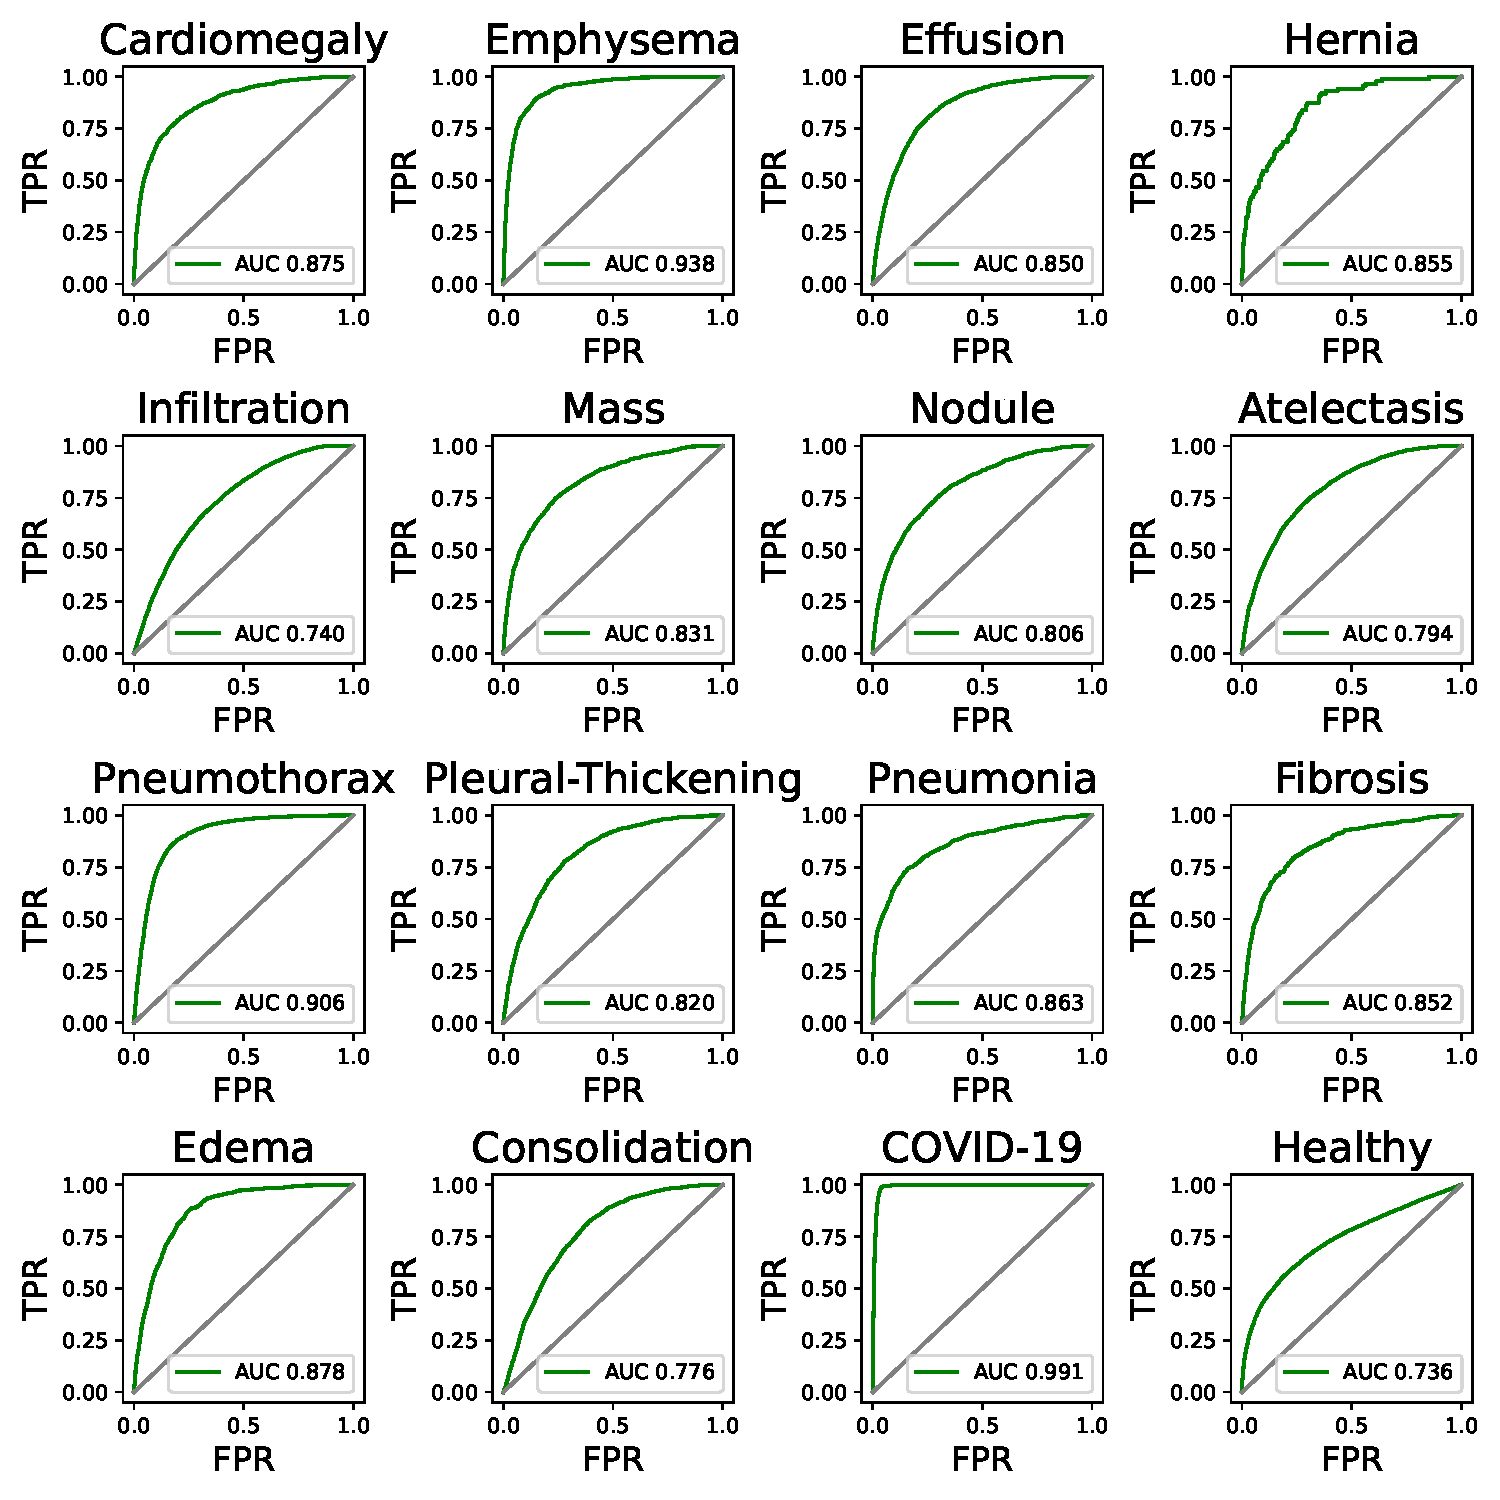
\includegraphics[width=1.5\textwidth]{Chapters/4. ViT-Lung/images/ROC_AUC.pdf}}
    \end{center}
    \caption{Curvas de ROC (gráficas de FPR contra TPR) para cada patología y muestras saludables
    del modelo CNN.}
    \label{roc-curves-cnn}
\end{figure}

\begin{figure}
    \begin{center}
        \scalebox{0.6}{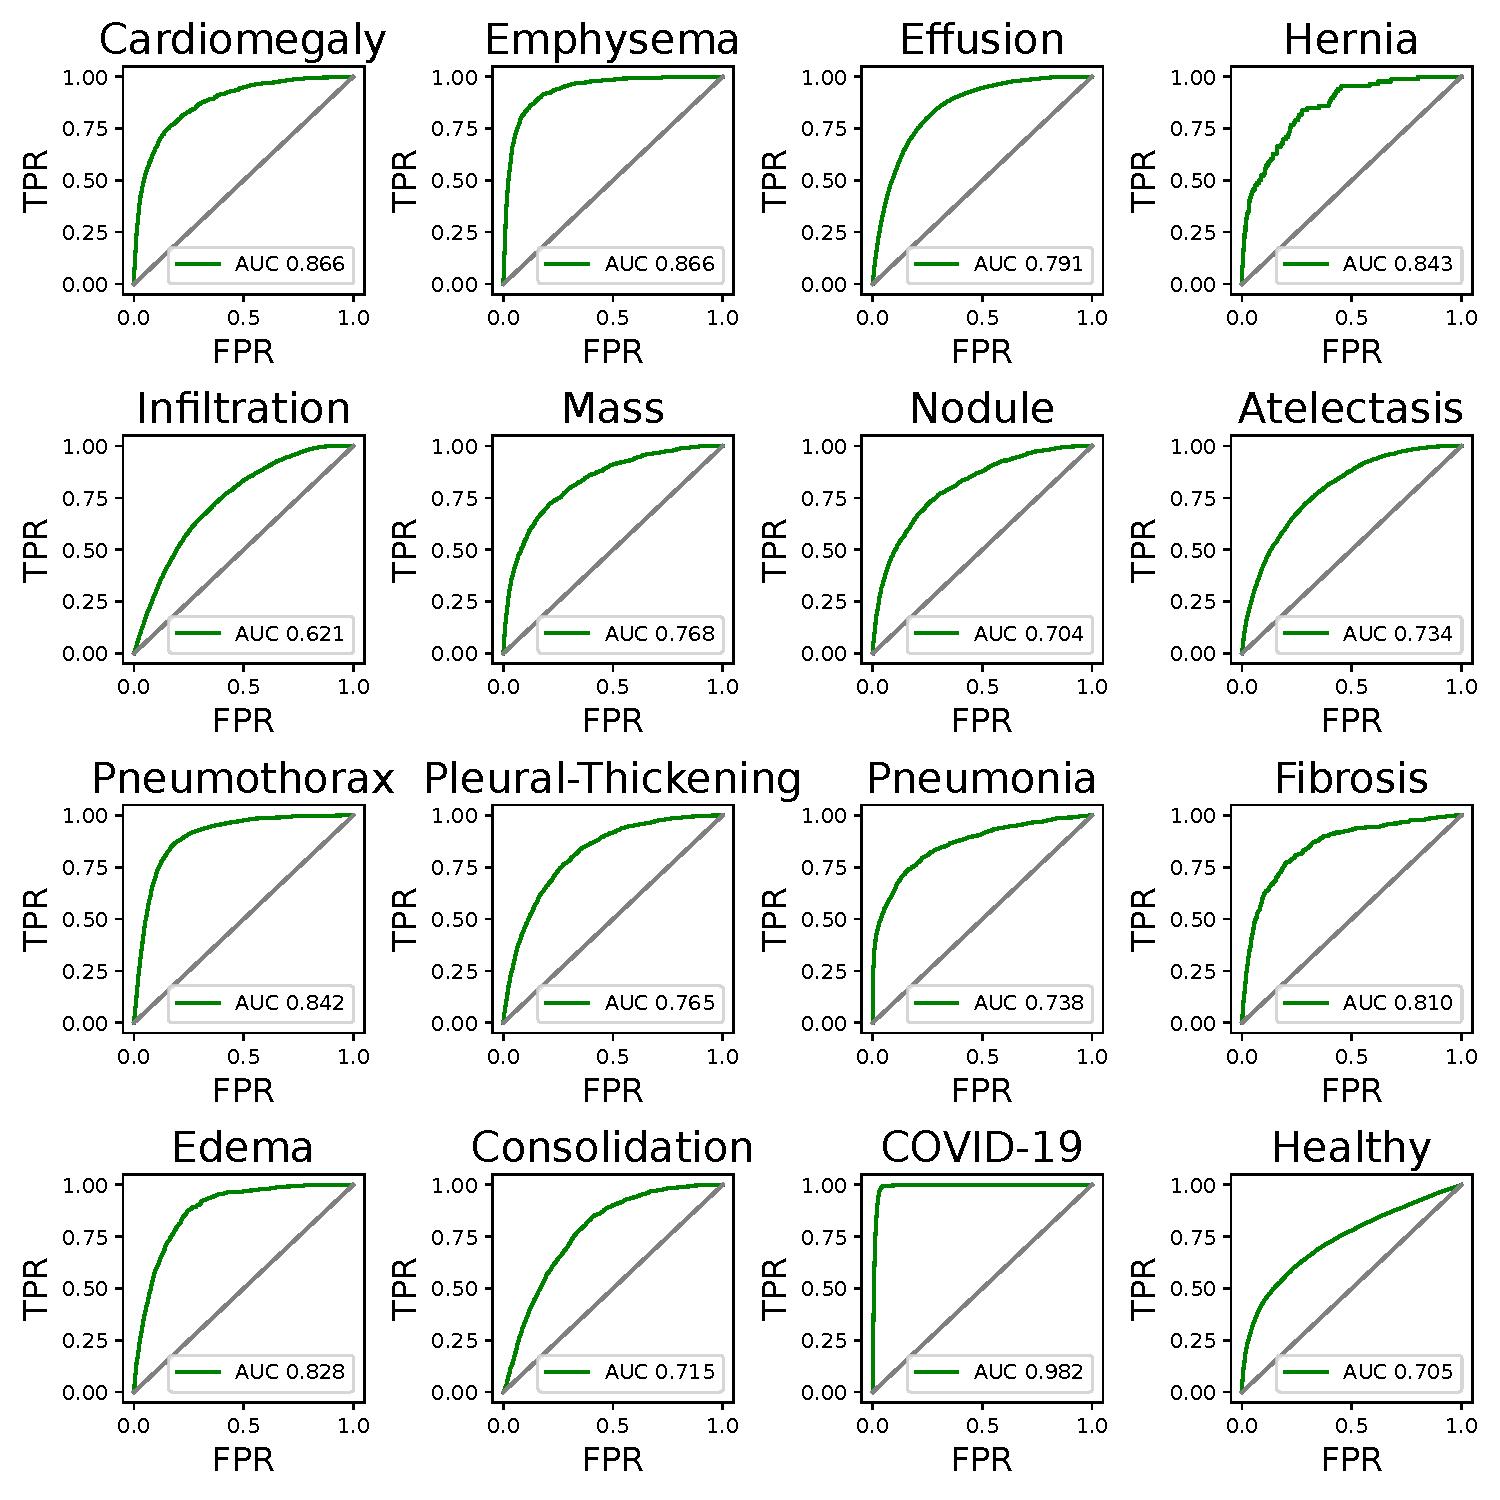
\includegraphics[width=1.5\textwidth]{Chapters/4. ViT-Lung/images/ROC_AUC_ViT.pdf}}
    \end{center}
    \caption{Curvas de ROC (gráficas de FPR contra TPR) para cada patología y muestras saludables
             del modelo ViT.}
    \label{roc-curves-vit}
\end{figure}

\begin{figure}[ht!]
    \centering
    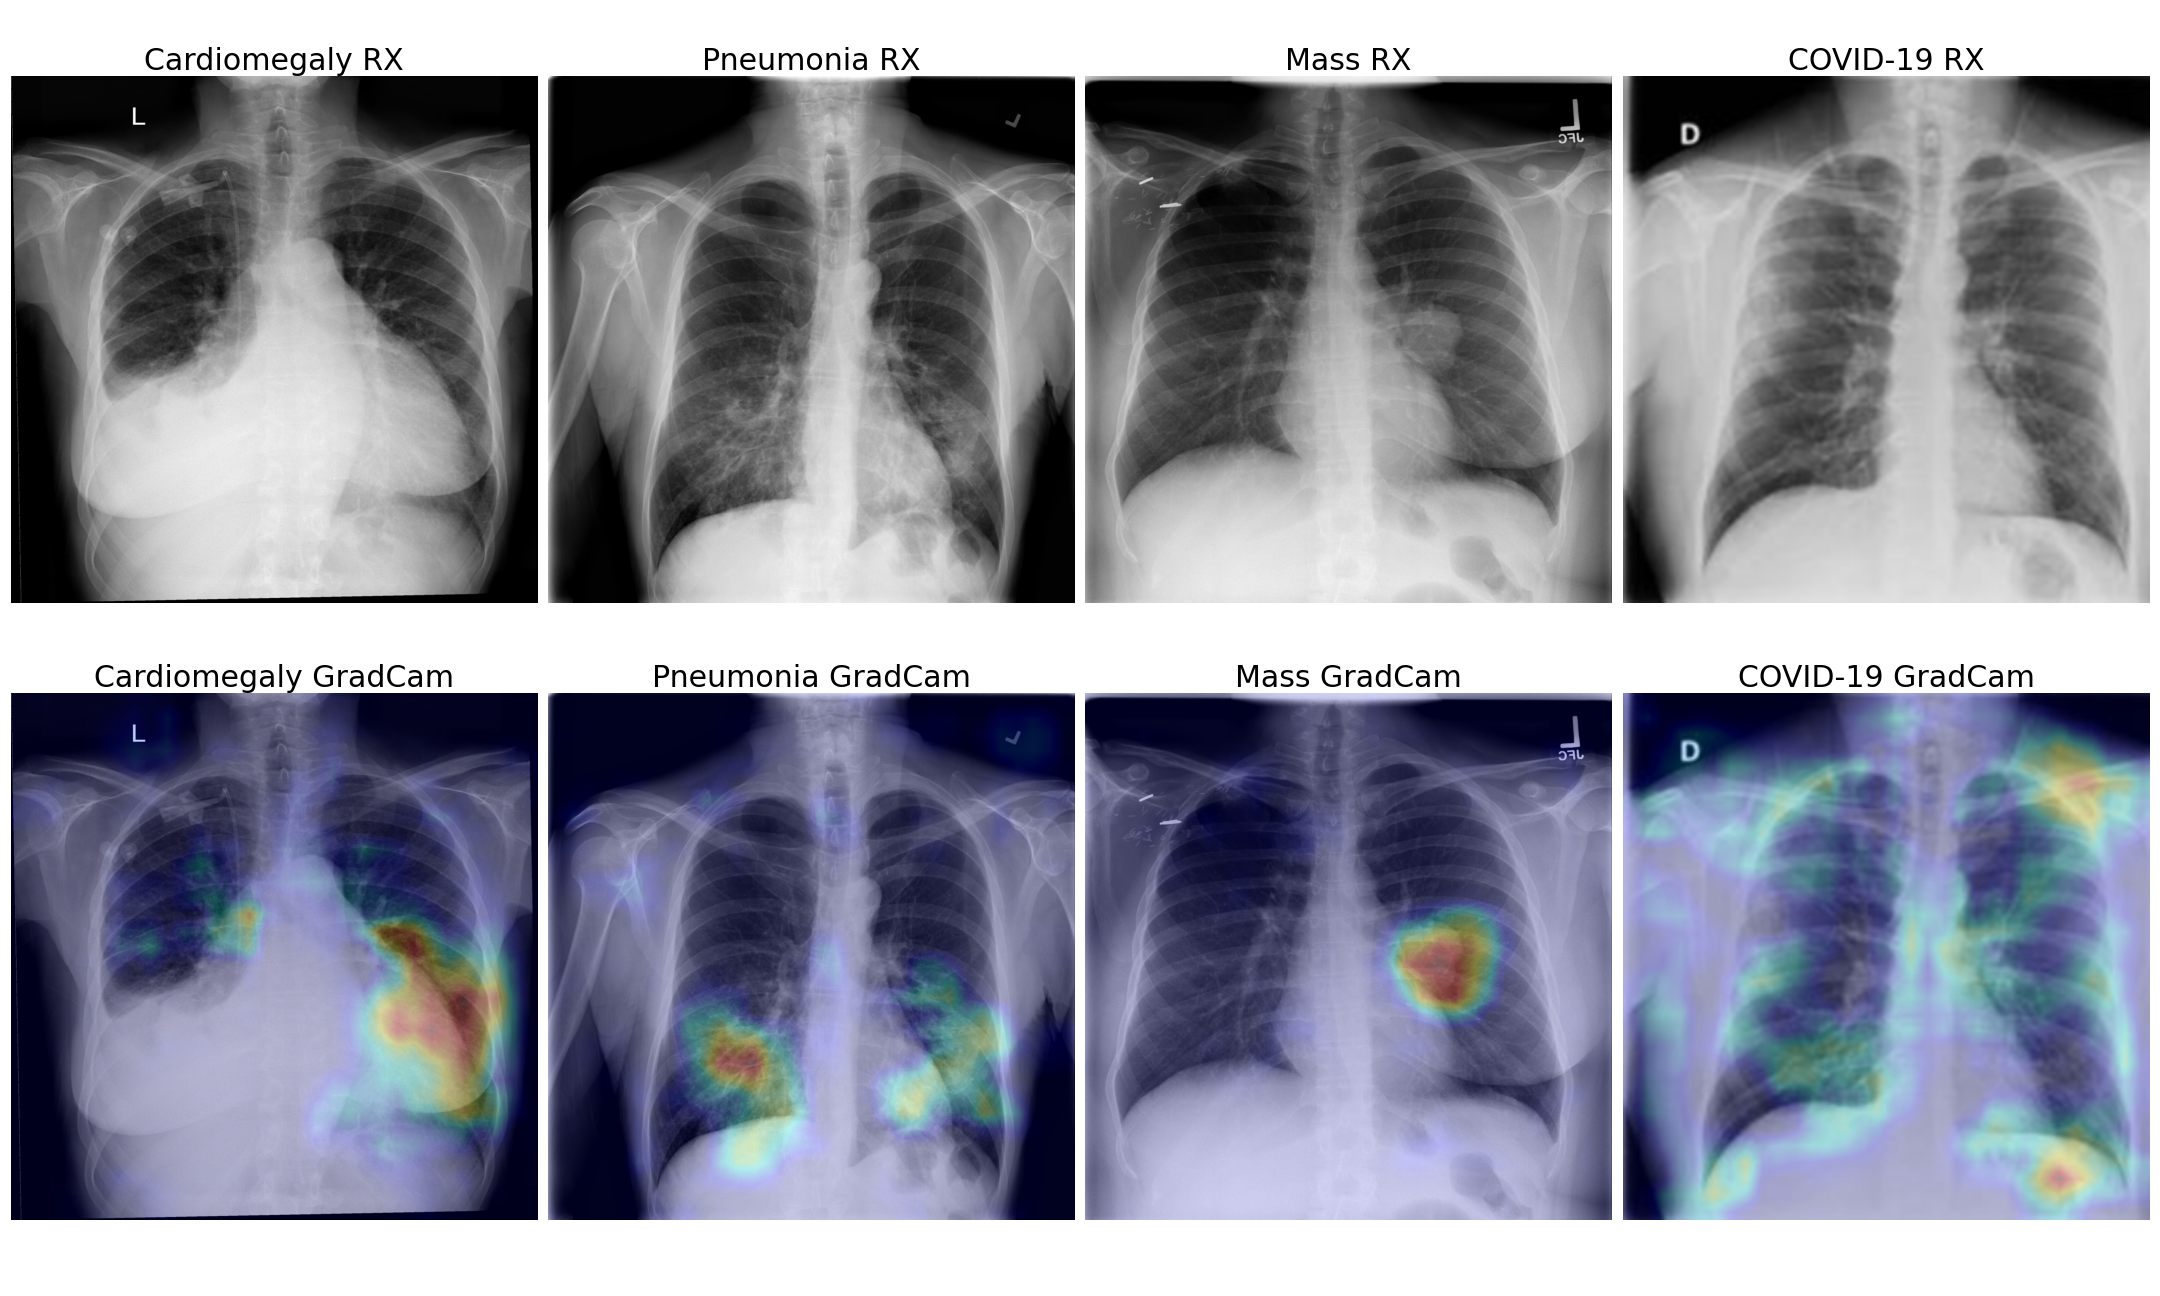
\includegraphics[width=0.8 \textwidth]{Chapters/4. ViT-Lung/images/vlgrid.png}
    \caption{Algunas imágenes de rayos-X (primer fila) con diferentes patologías y sus imágenes GradCam
             asociadas en la segunda fila. La primera columna muestra un corazón crecido, la segunda
             columna corresponde a neumonía, la tercer columna muestra una especie de tejido inusual
             en el pulmón y la última columna un caso de COVID-19.}
    \label{img-results}
\end{figure}

De manera general, el rendimiento del modelo convolucional basado en \textit{ResNet50} es mayor al
modelo de atención basado en \textit{ViT}. Cabe resaltar que solo existe una diferencia en ambos modelos
que podría mejorar los resultados en favor del modelo \textit{ViT}: la resolución de las imágenes. El
modelo \textit{ViT} trabaja con imágenes más pequeñas que el modelo \textit{ResNet50}, $384\times384$ y
$1024\times1024$ respectivamente. Dicha limitante se debe a la capacidad computacional requerida y con la
que se contó para el entrenamiento, ya que el modelo basado en \textit{ViT} requiere un consumo de memoria
mucho mayor para su procesamiento.


\begin{figure}[b]
    \centering
    \begin{subfigure}{0.4\textwidth}
        \centering
        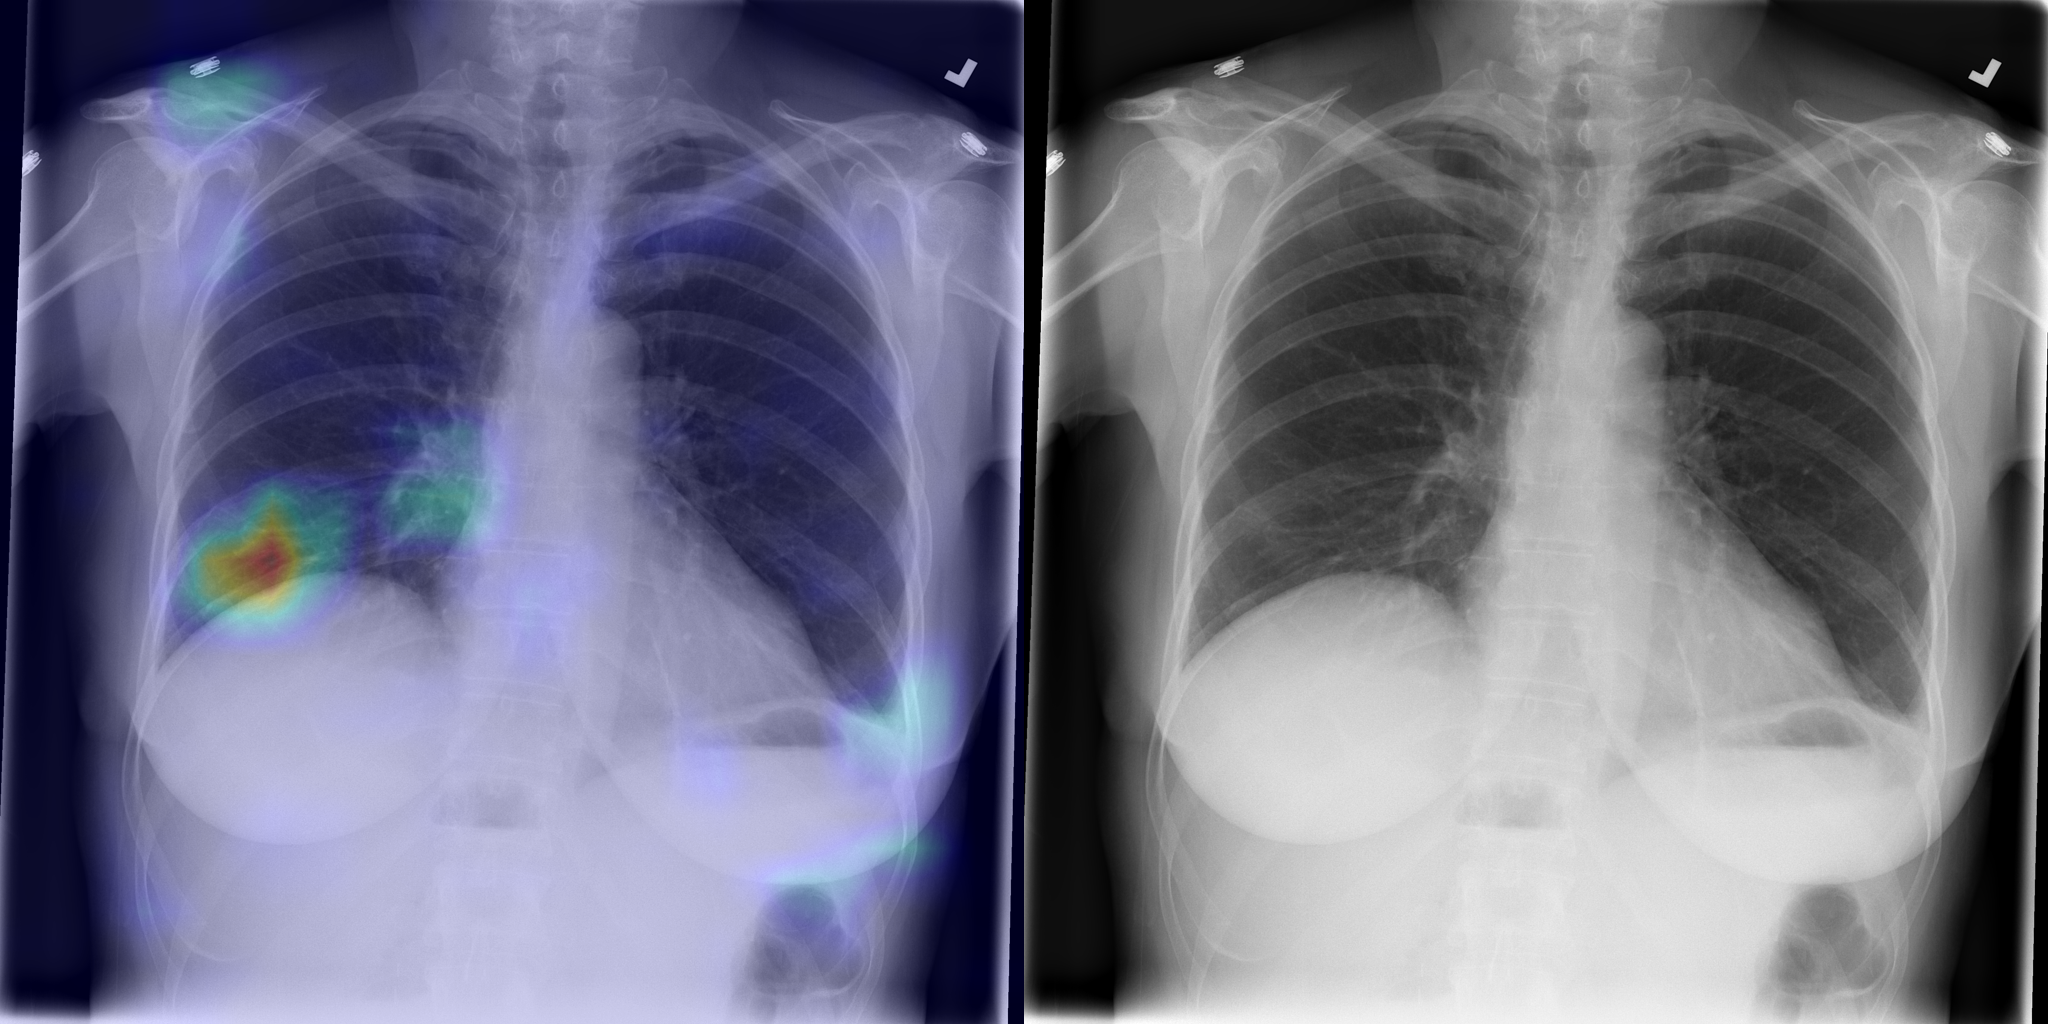
\includegraphics[width=1.0\textwidth]{Chapters/5. Conclusiones/img/Atelectasis/1_1_00000147_001.png}
    \end{subfigure}
    \begin{subfigure}{0.4\textwidth}
        \centering
        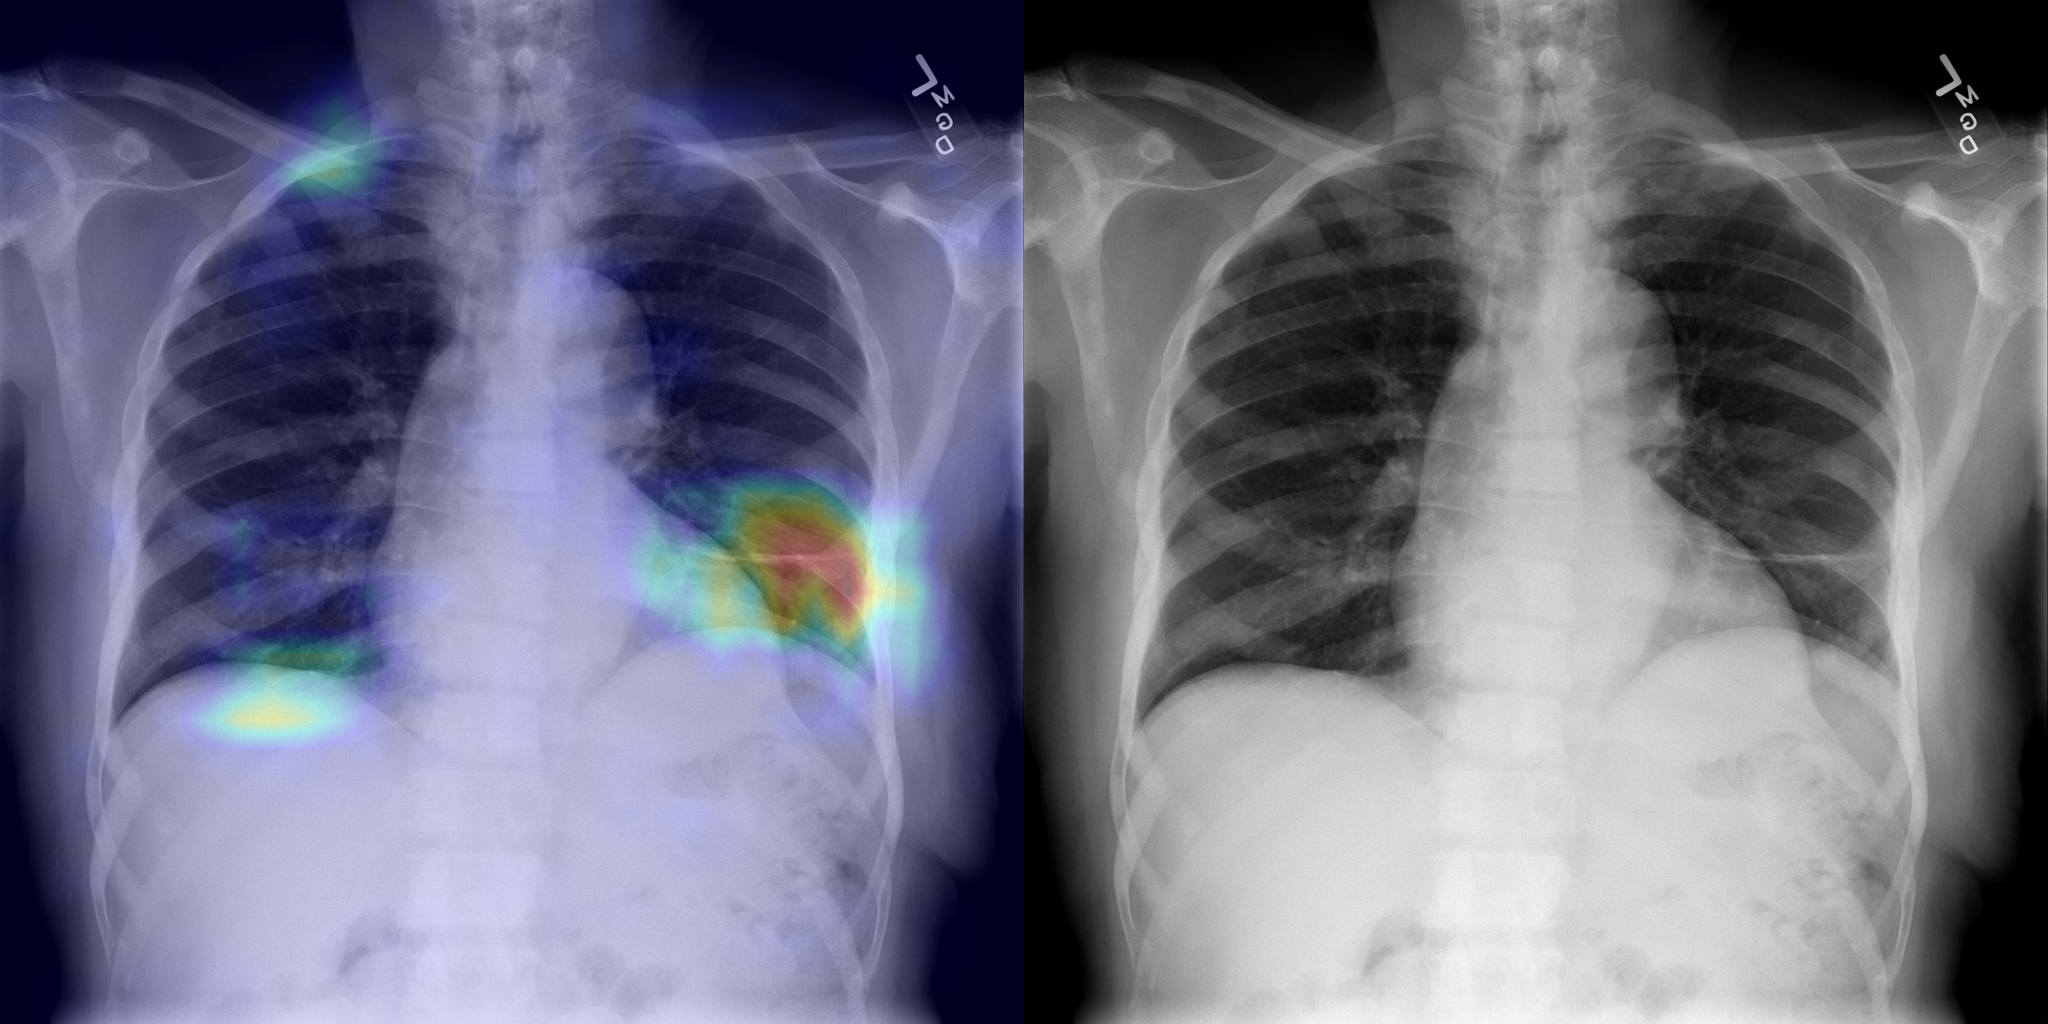
\includegraphics[width=1.0\textwidth]{Chapters/5. Conclusiones/img/Atelectasis/1_1_00000149_002.png}
    \end{subfigure}
    \begin{subfigure}{0.4\textwidth}
        \centering
        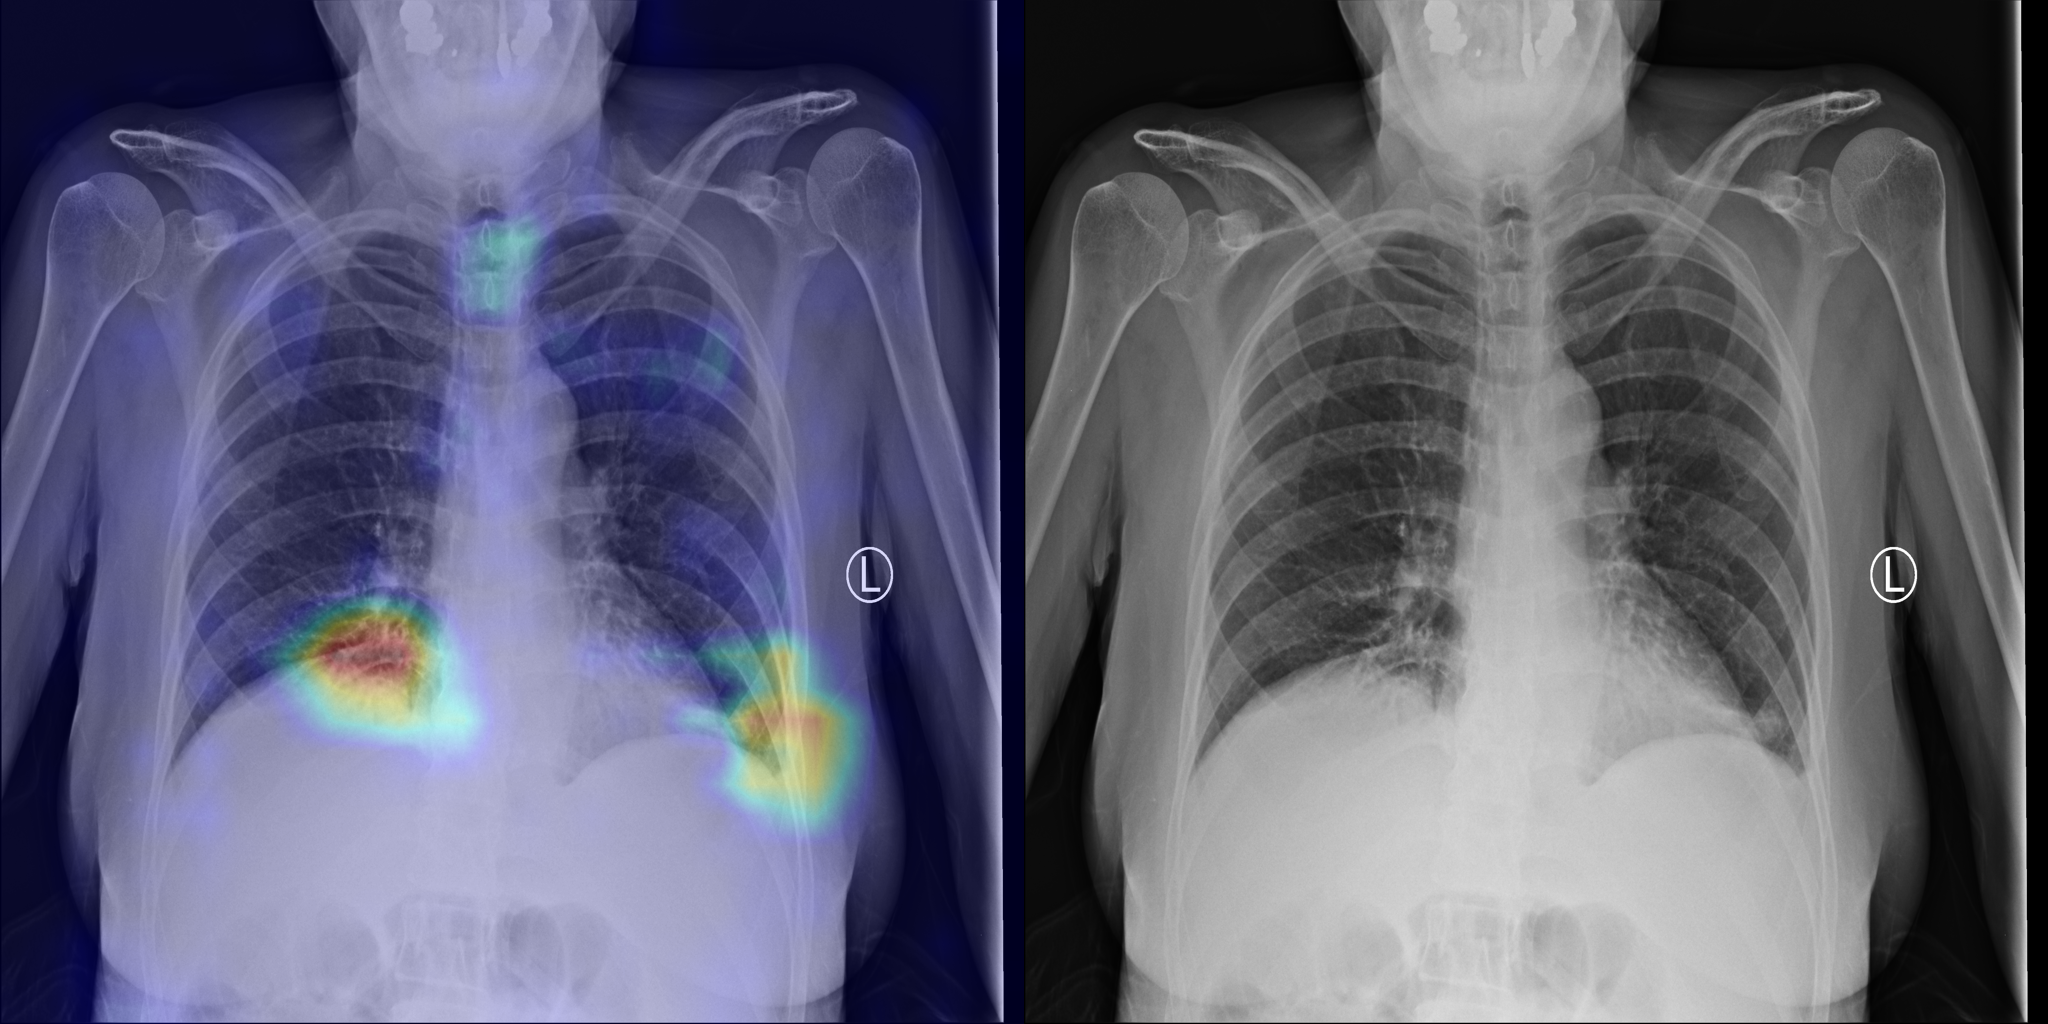
\includegraphics[width=1.0\textwidth]{Chapters/5. Conclusiones/img/Atelectasis/1_1_00000150_003.png}
    \end{subfigure}
    \begin{subfigure}{0.4\textwidth}
        \centering
        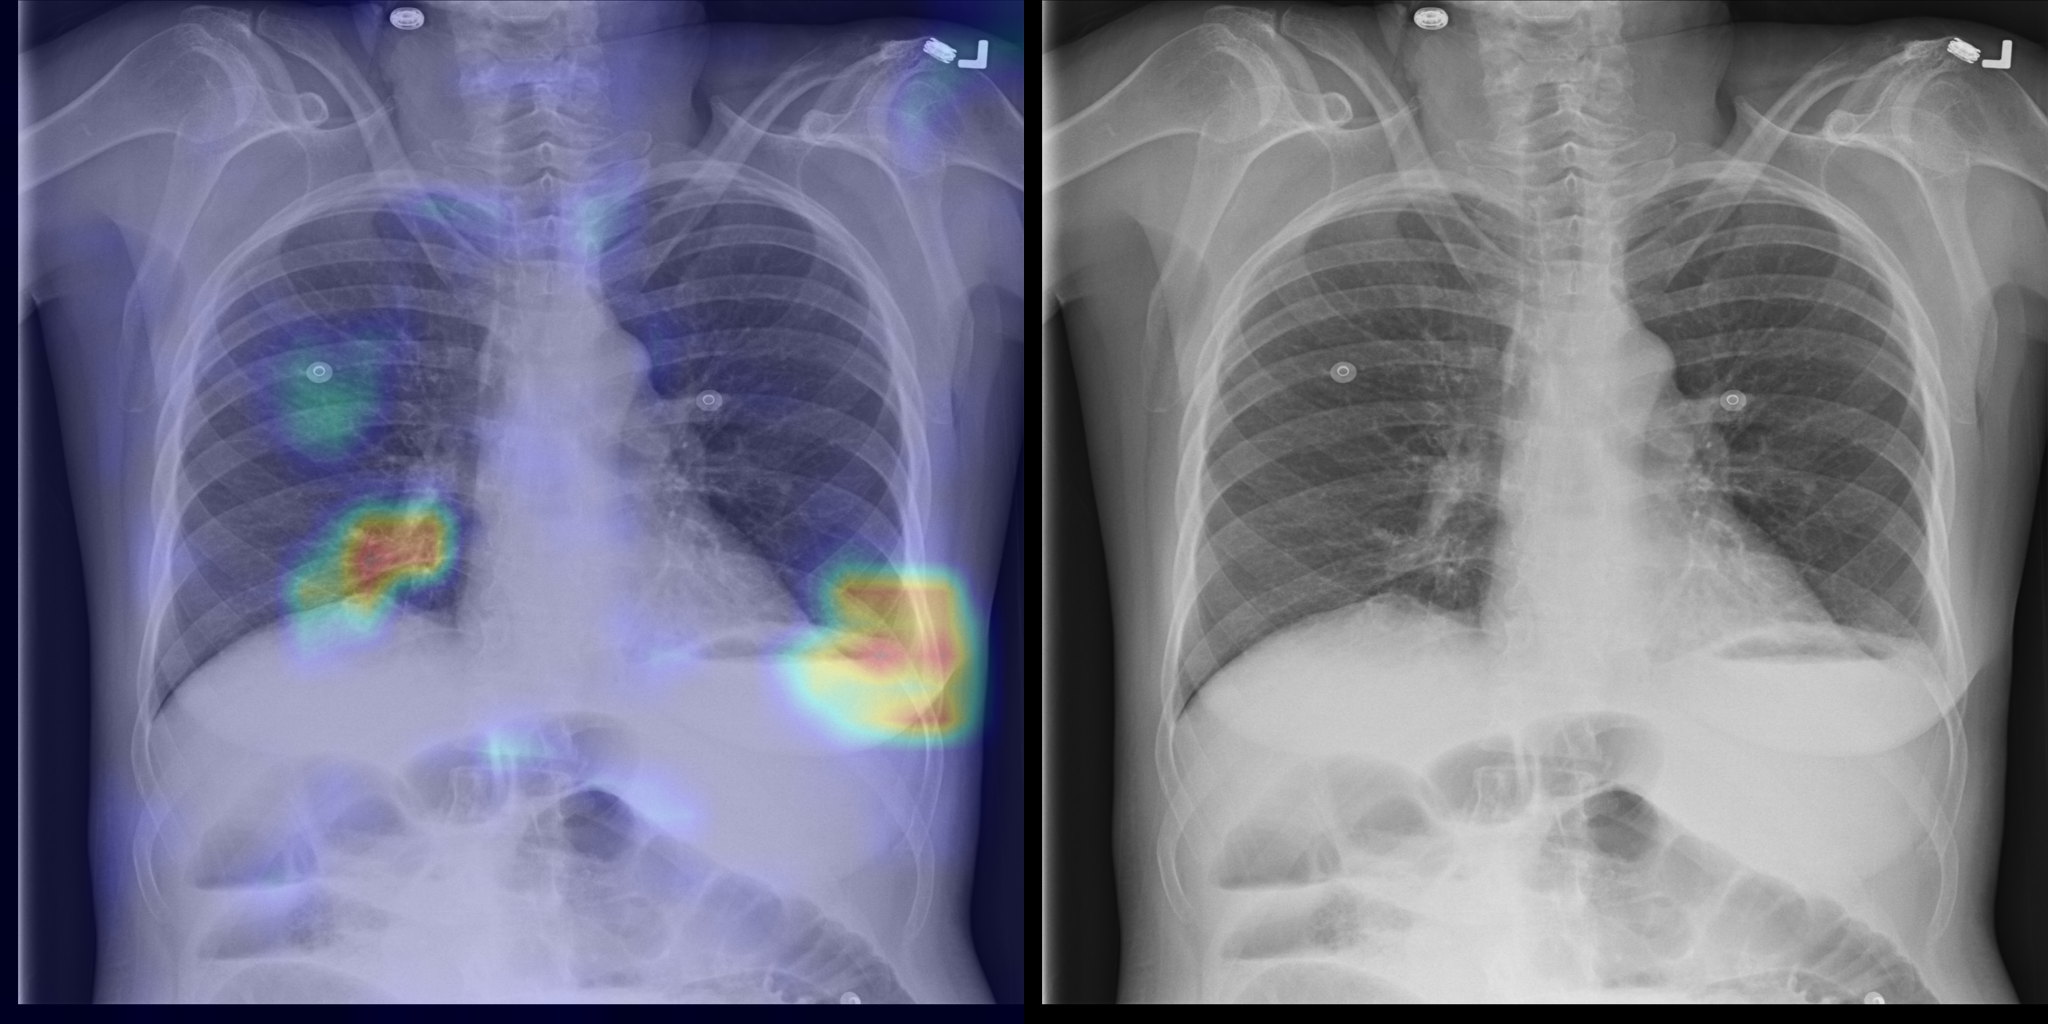
\includegraphics[width=1.0\textwidth]{Chapters/5. Conclusiones/img/Atelectasis/1_1_00000150_004.png}
    \end{subfigure}
    \begin{subfigure}{0.4\textwidth}
        \centering
        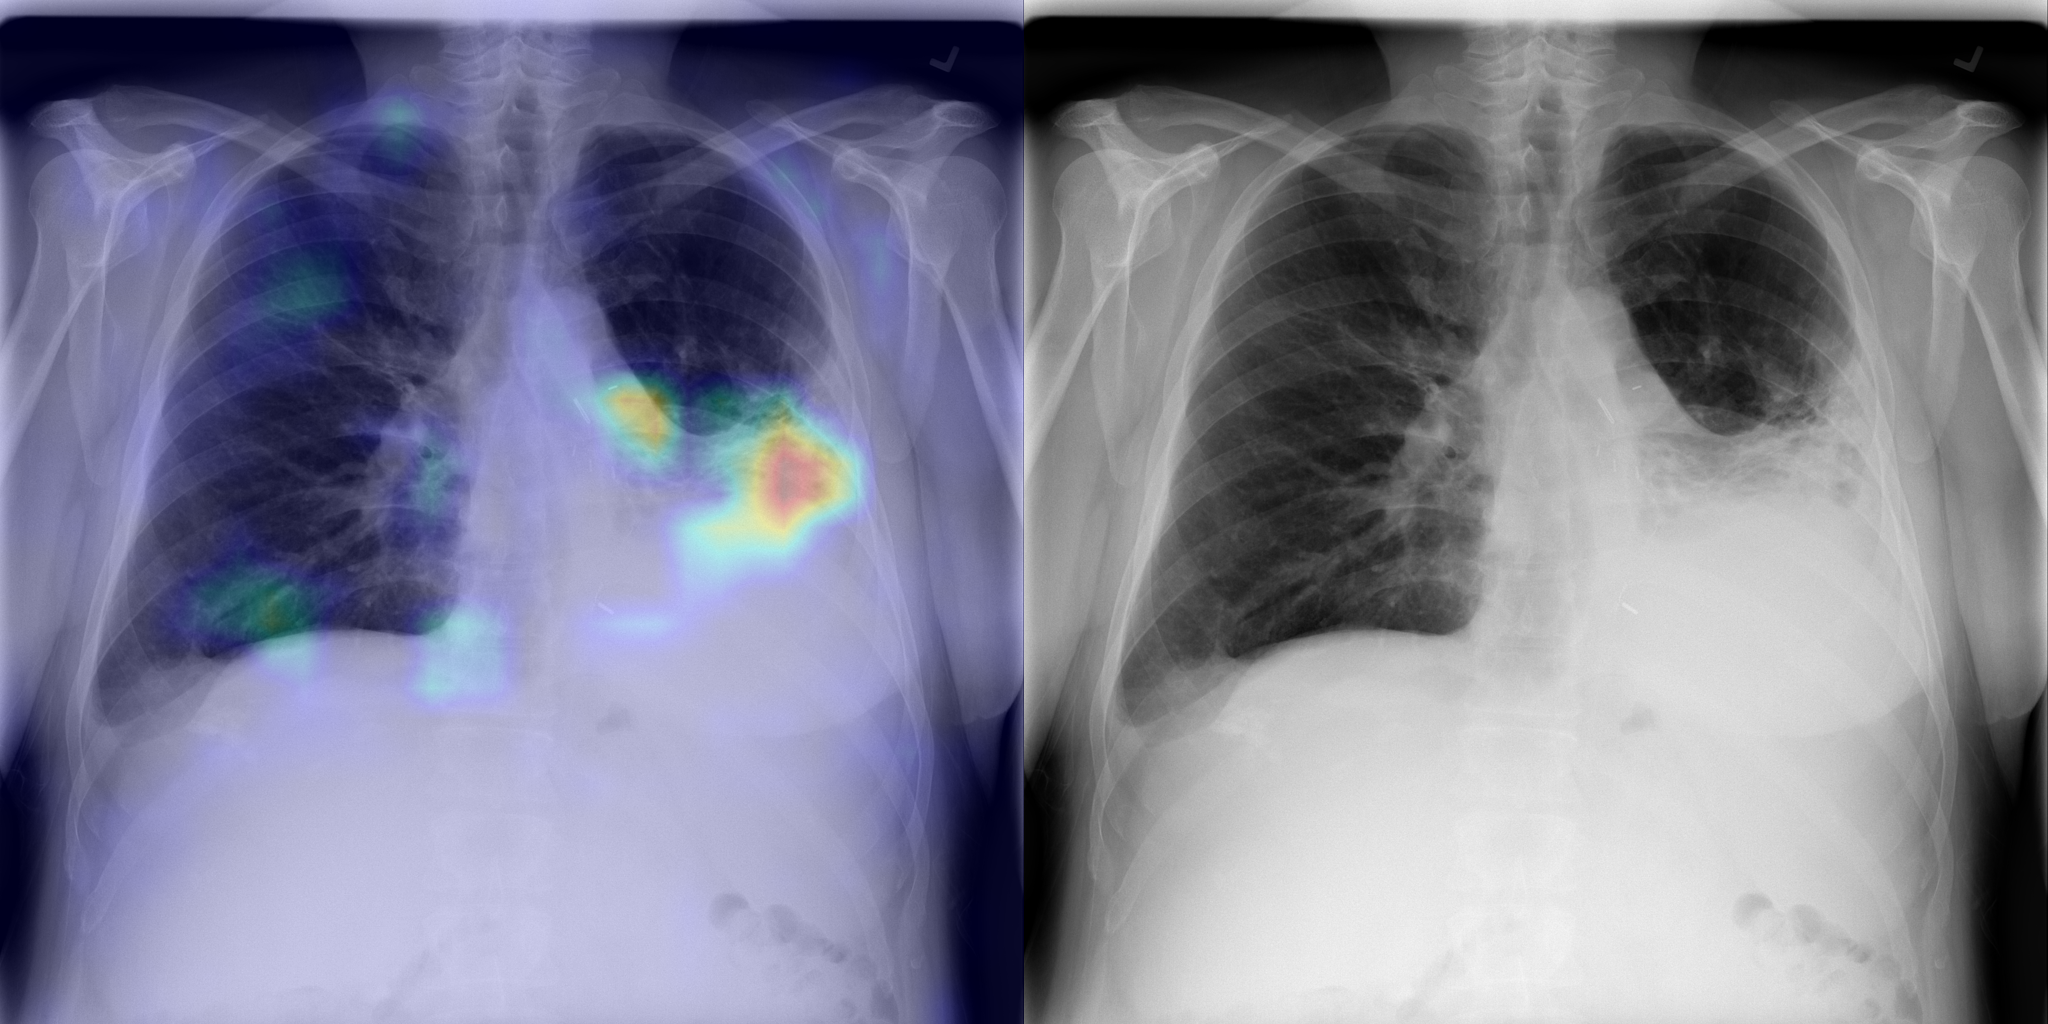
\includegraphics[width=1.0\textwidth]{Chapters/5. Conclusiones/img/Atelectasis/1_1_00000467_000.png}
    \end{subfigure}
    \begin{subfigure}{0.4\textwidth}
        \centering
        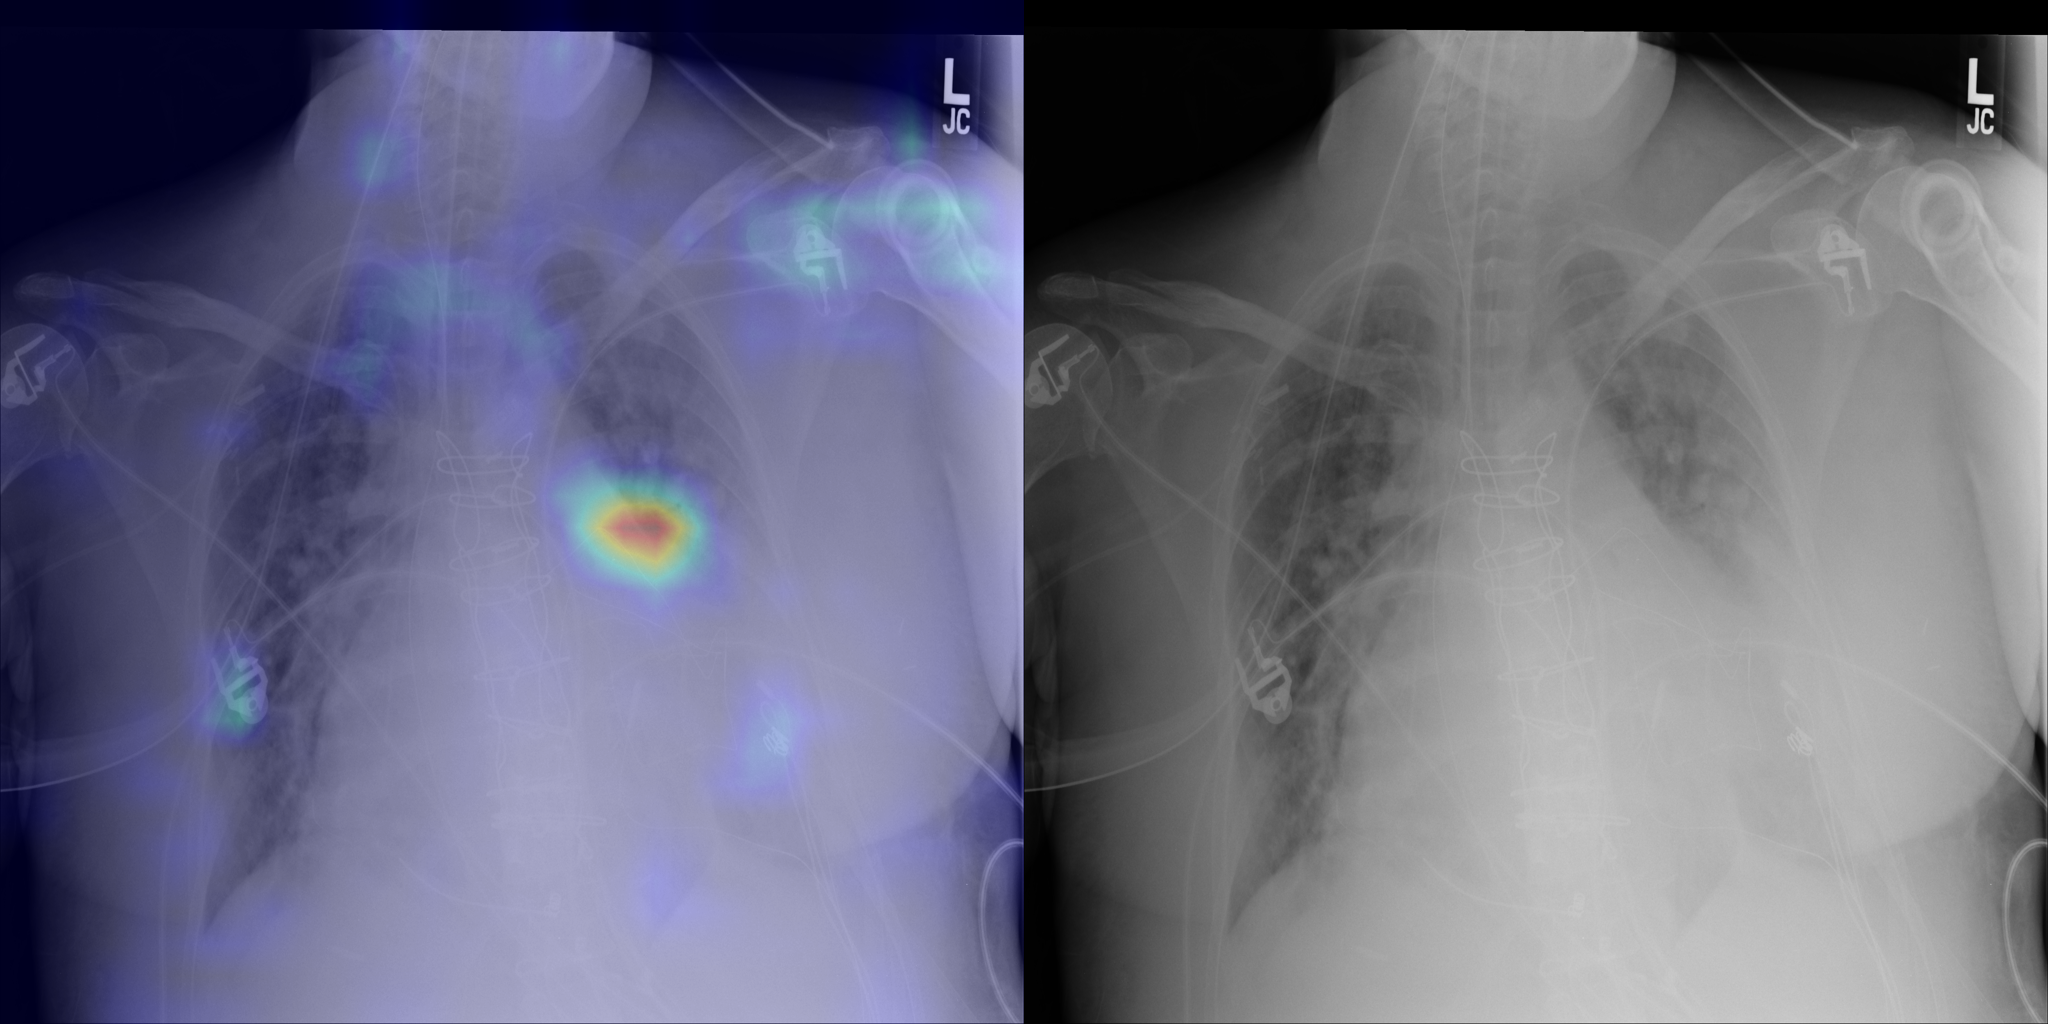
\includegraphics[width=1.0\textwidth]{Chapters/5. Conclusiones/img/Atelectasis/1_1_00000032_036.png}
    \end{subfigure}
    \begin{subfigure}{0.4\textwidth}
        \centering
        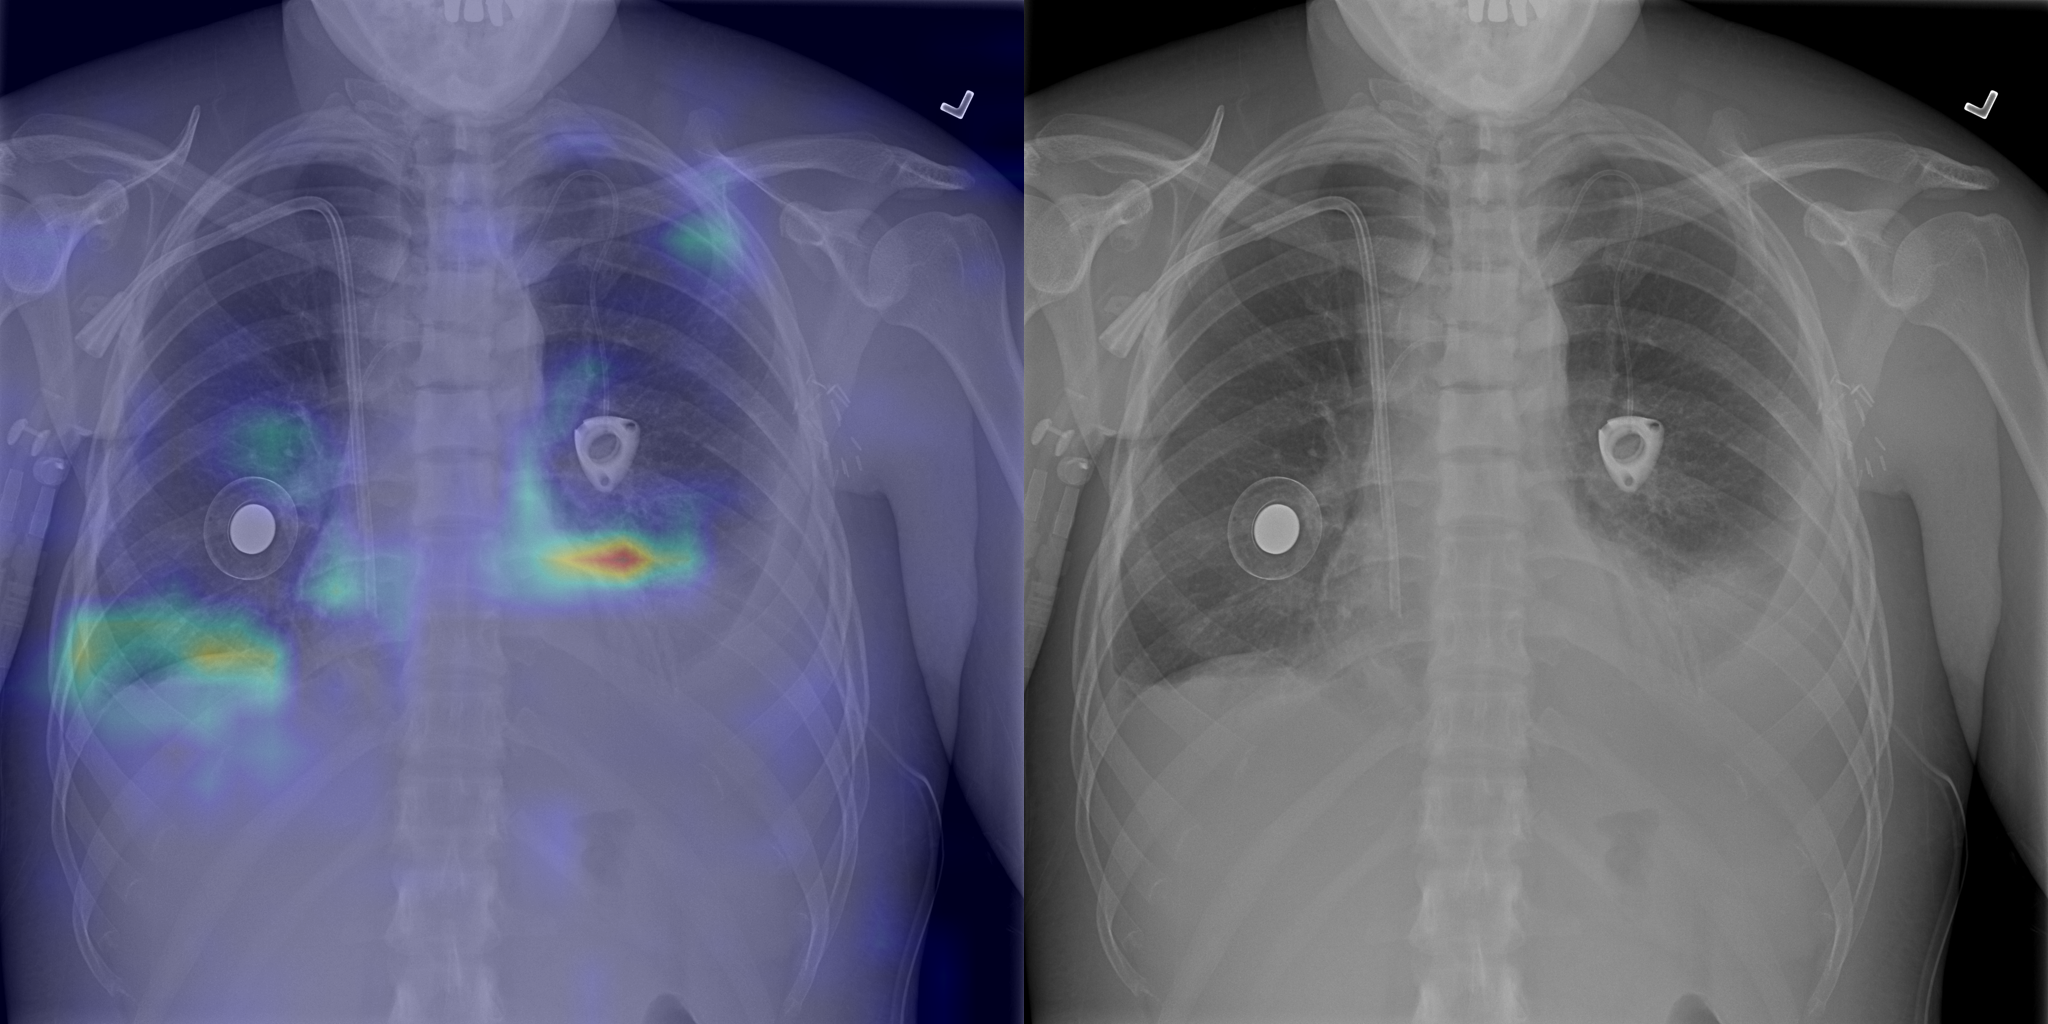
\includegraphics[width=1.0\textwidth]{Chapters/5. Conclusiones/img/Atelectasis/1_1_00029596_022.png}
    \end{subfigure}
    \begin{subfigure}{0.4\textwidth}
        \centering
        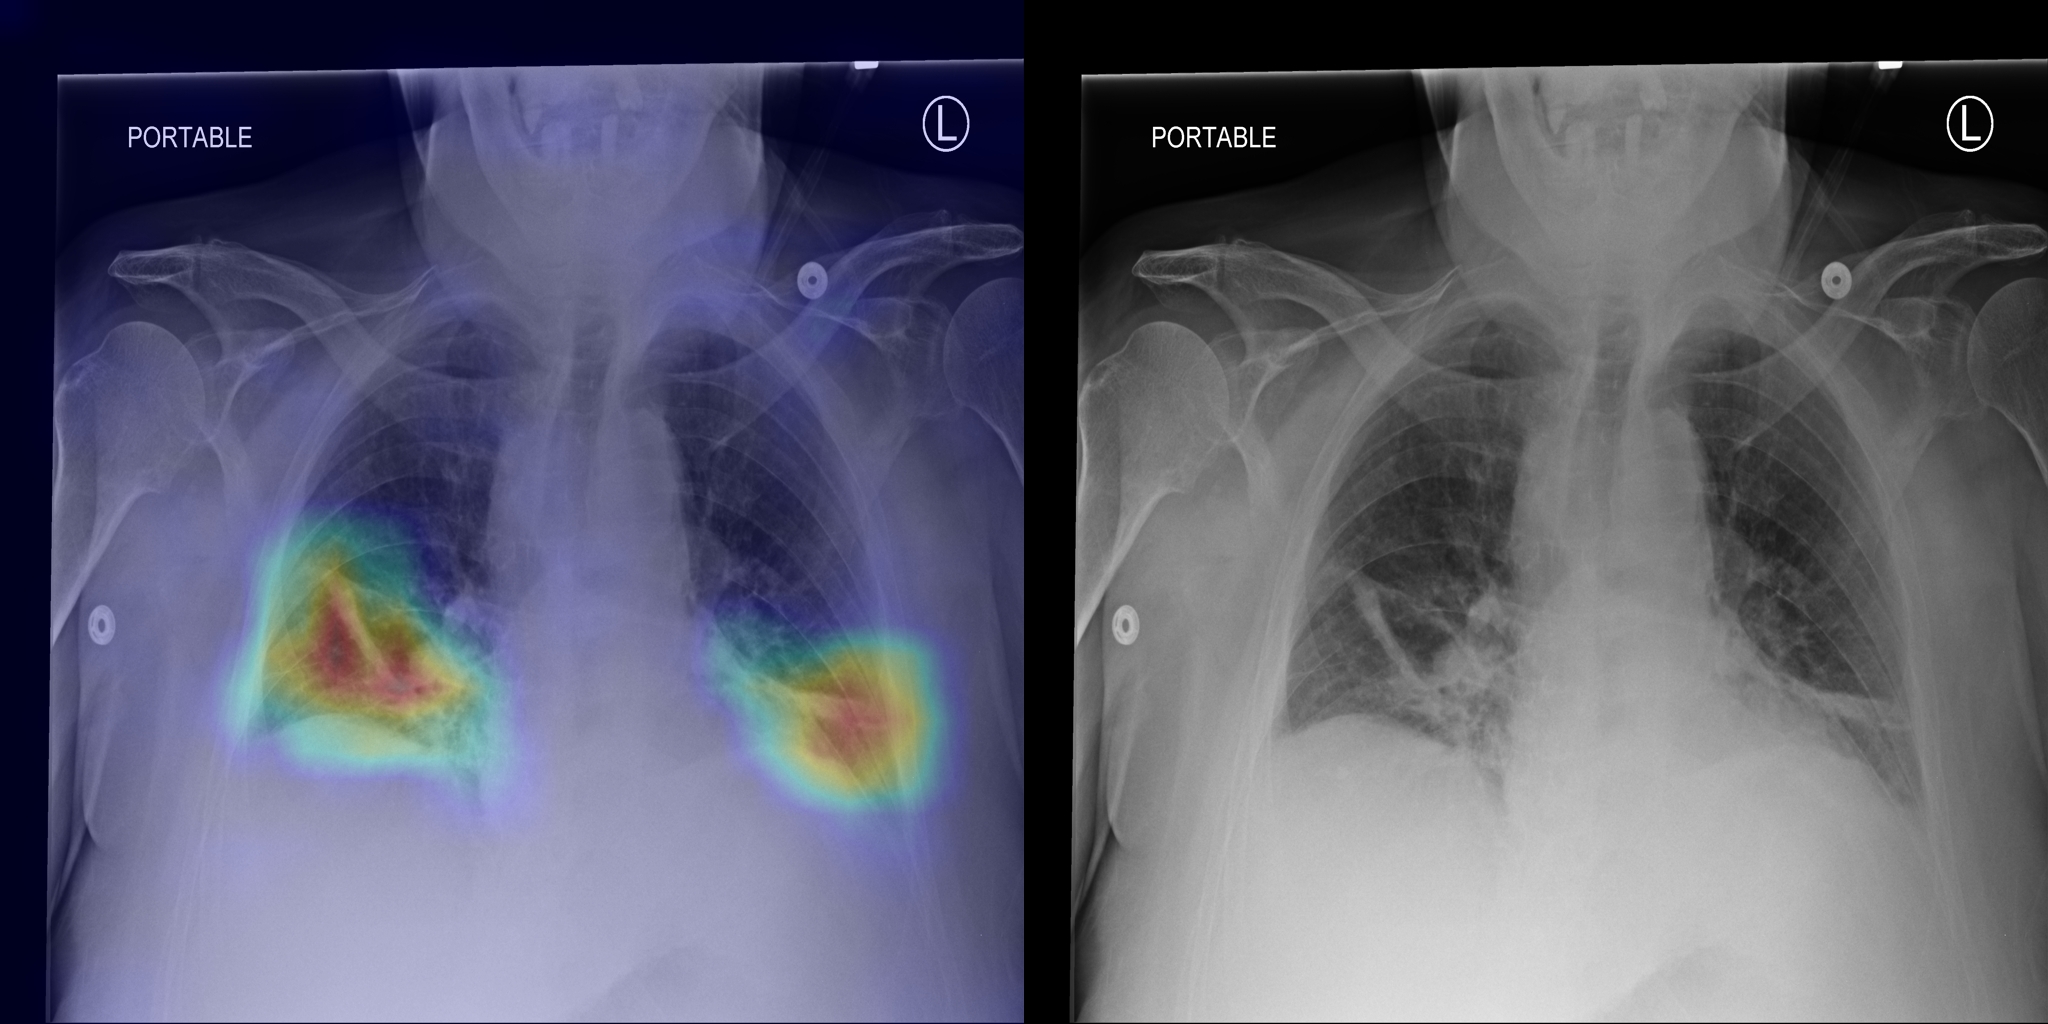
\includegraphics[width=1.0\textwidth]{Chapters/5. Conclusiones/img/Atelectasis/1_1_00030408_000.png}
    \end{subfigure}
    \begin{subfigure}{0.4\textwidth}
        \centering
        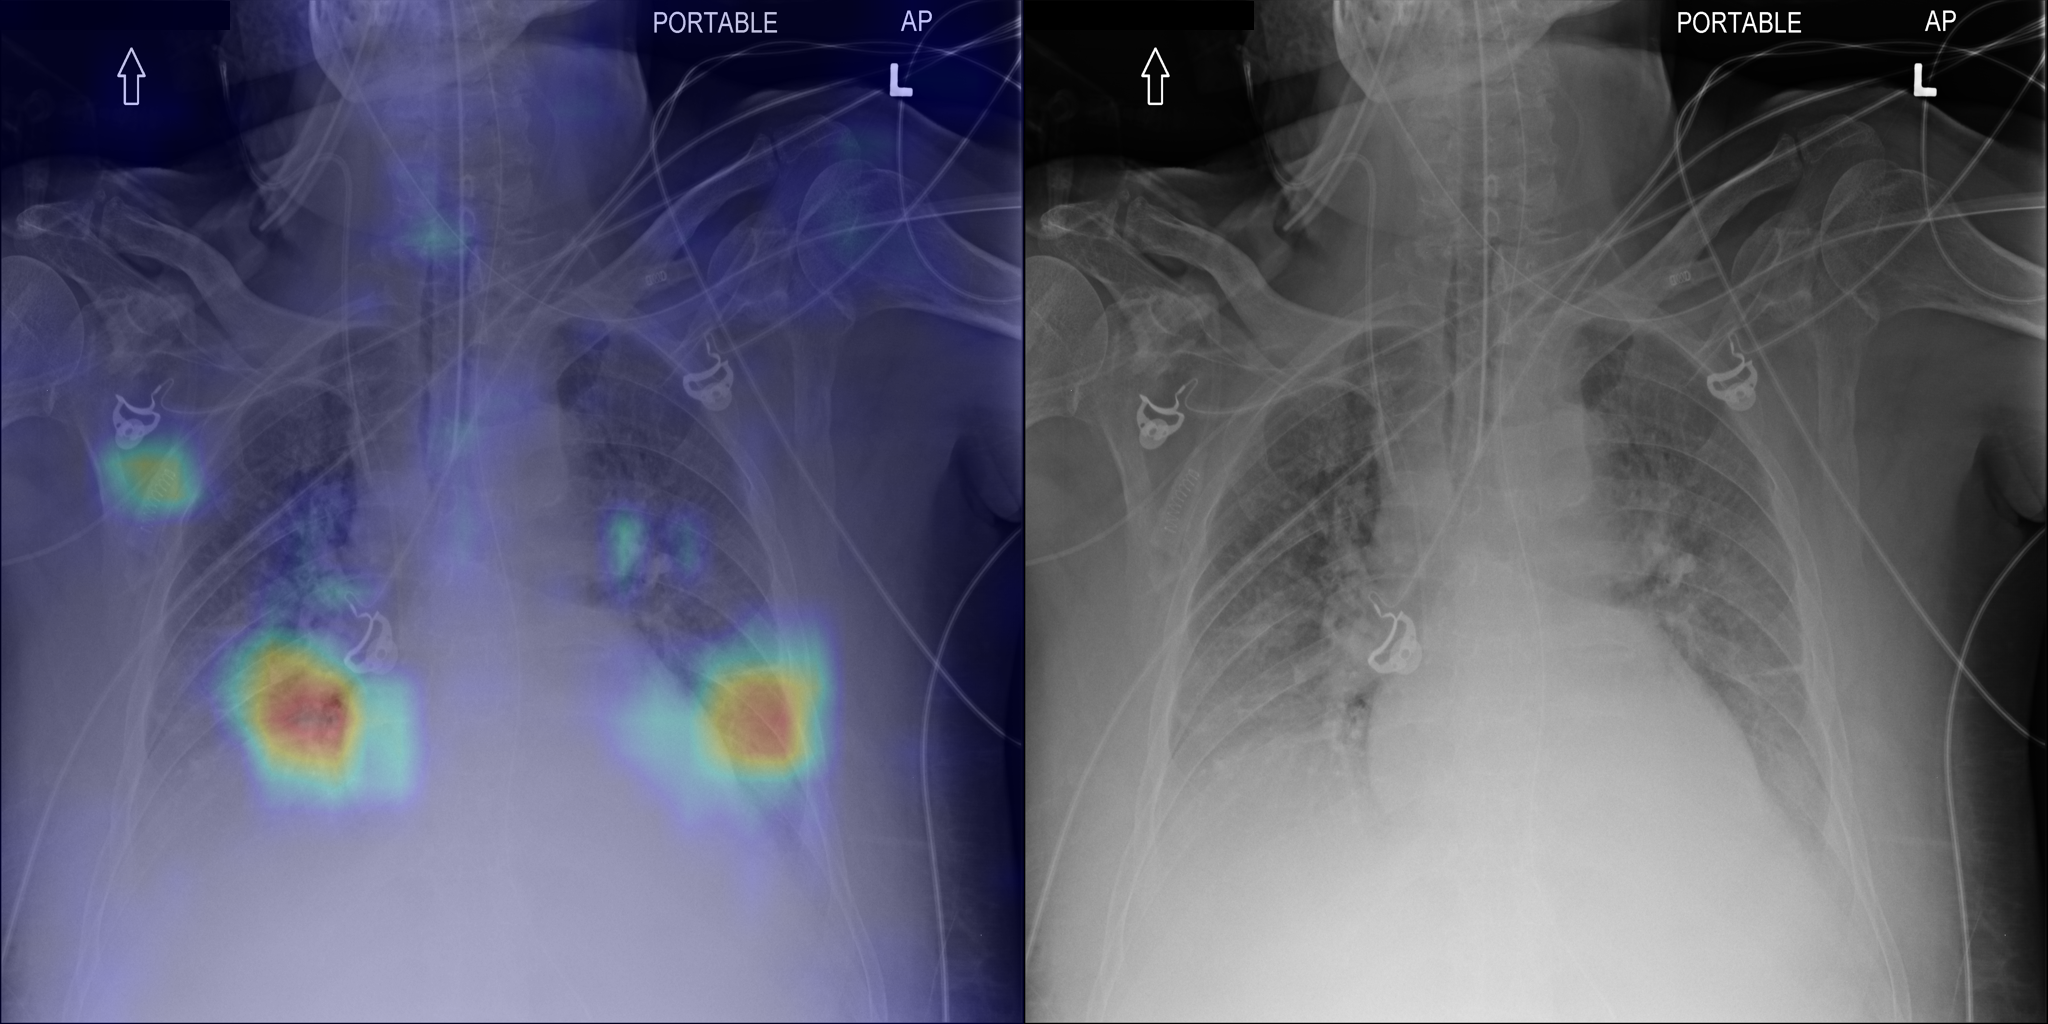
\includegraphics[width=1.0\textwidth]{Chapters/5. Conclusiones/img/Atelectasis/1_1_00030408_013.png}
    \end{subfigure}
    \begin{subfigure}{0.4\textwidth}
        \centering
        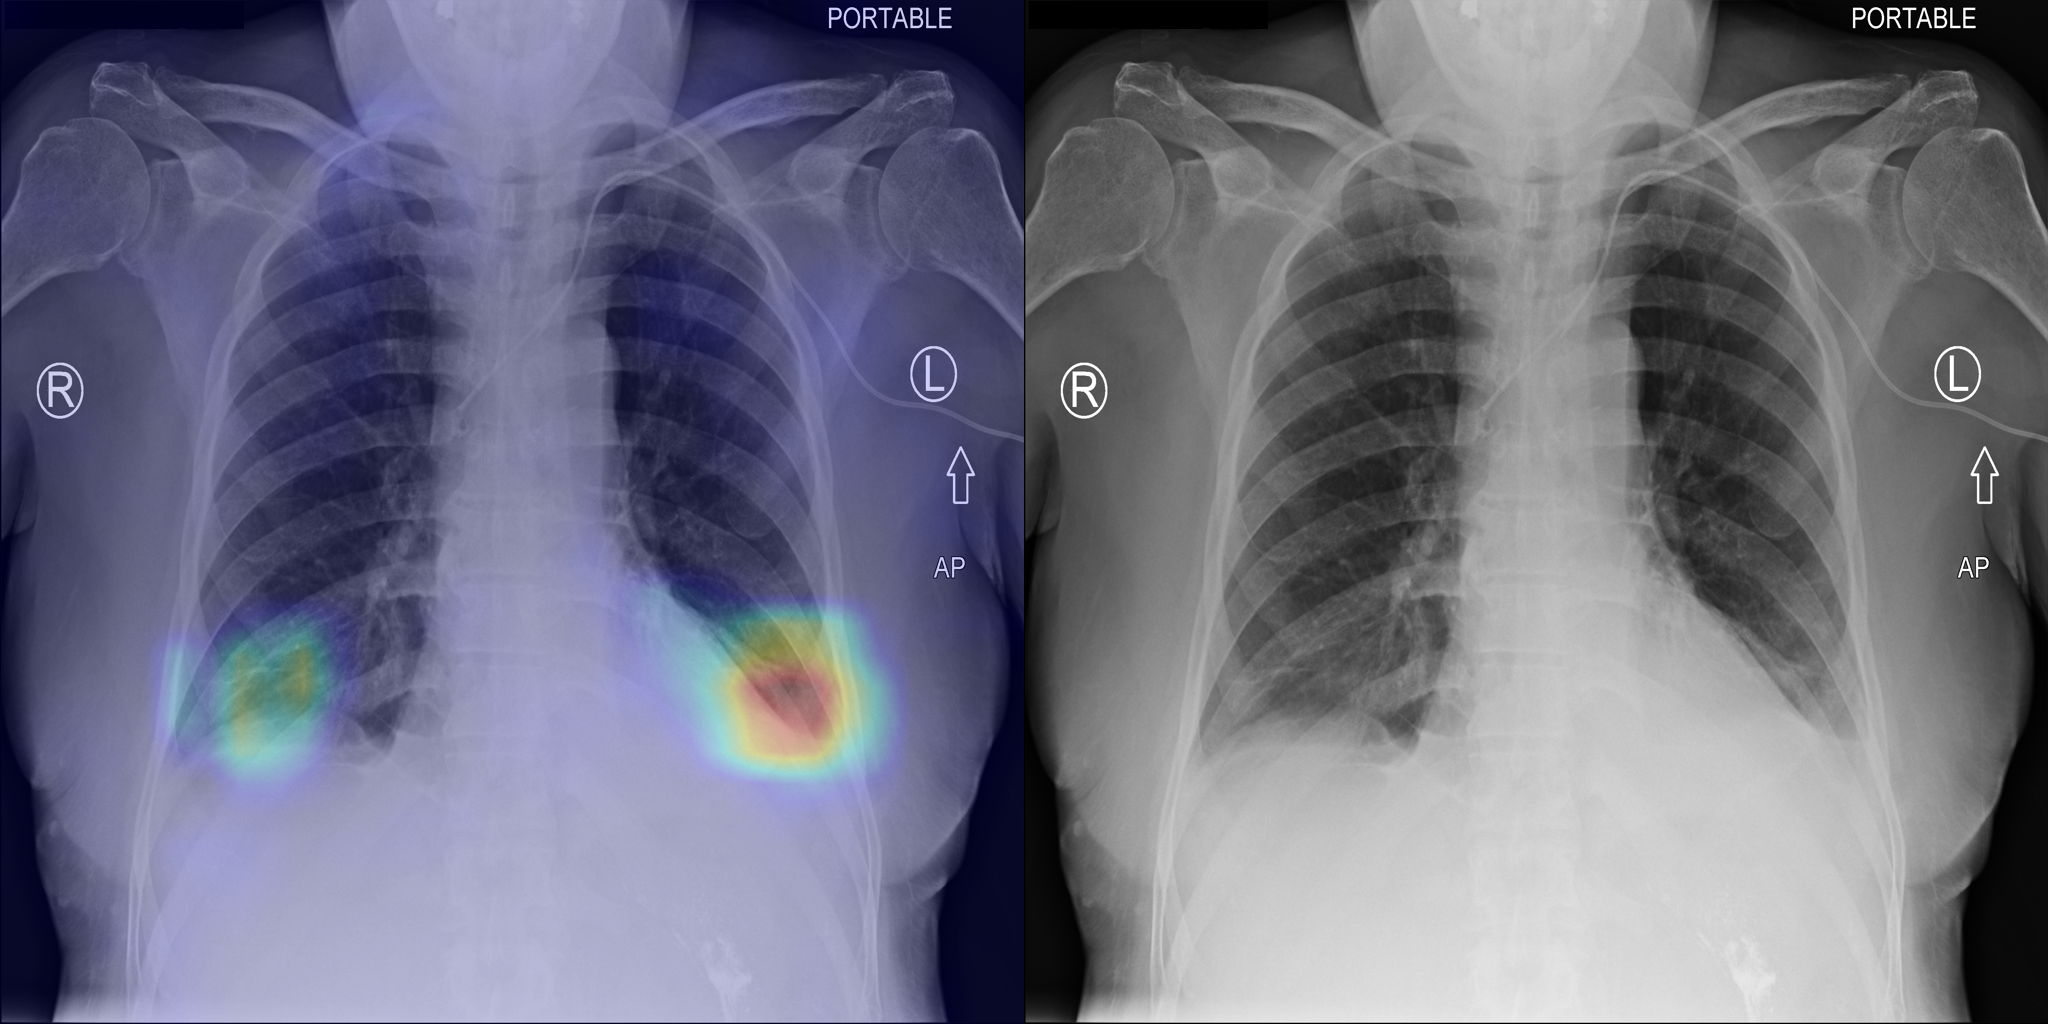
\includegraphics[width=1.0\textwidth]{Chapters/5. Conclusiones/img/Atelectasis/1_1_00028974_018.png}
    \end{subfigure}

    \caption{Atelectasis. Radiografías detectadas con la patología de atelectasis por los
                    radiólogos. A la izquierda de cada imagen el GradCam correspondiente a la detección
                    de la patología como positivo por el modelo CNN.}
    \label{fig-atelectasis}
\end{figure}

\begin{figure}[b]
    \centering
    \begin{subfigure}{0.4\textwidth}
        \centering
        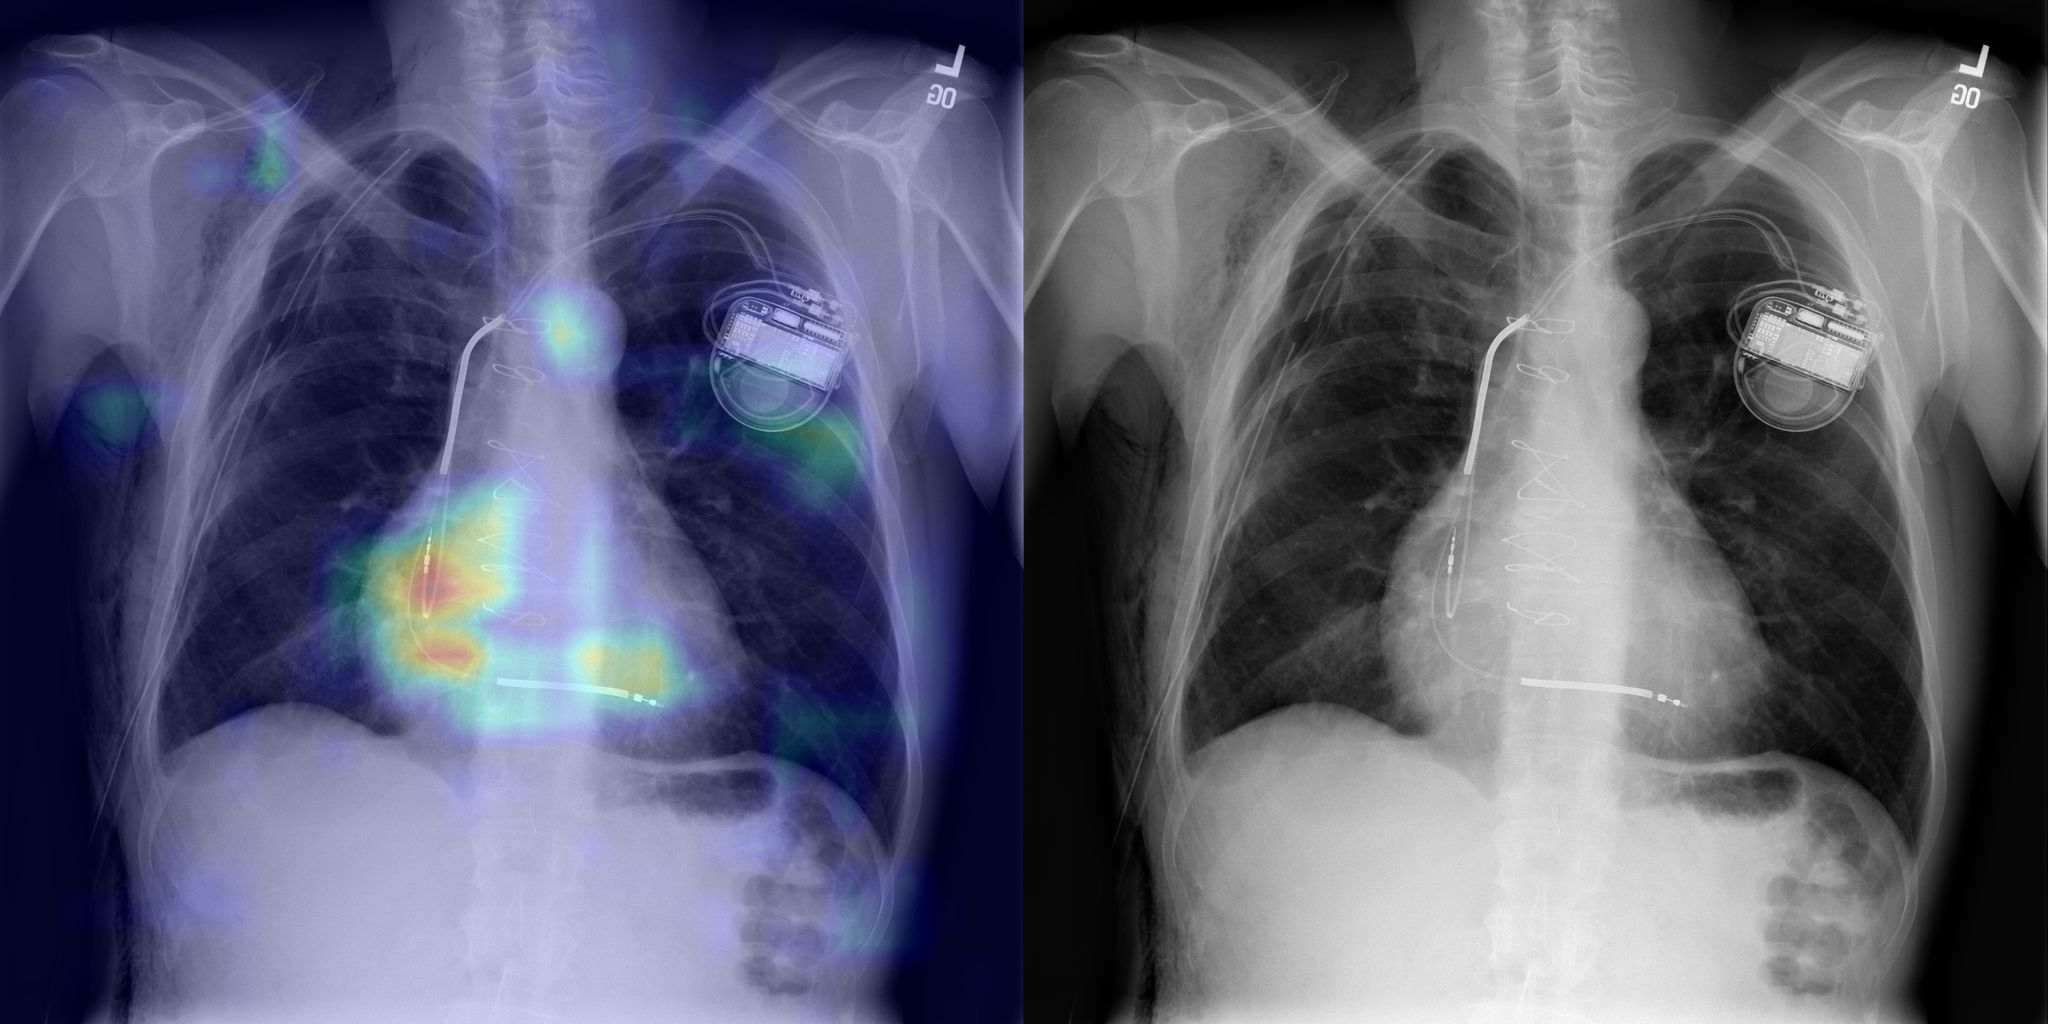
\includegraphics[width=1.0\textwidth]{Chapters/5. Conclusiones/img/Cardiomegaly/1_0_00000013_037.png}
    \end{subfigure}
    \begin{subfigure}{0.4\textwidth}
        \centering
        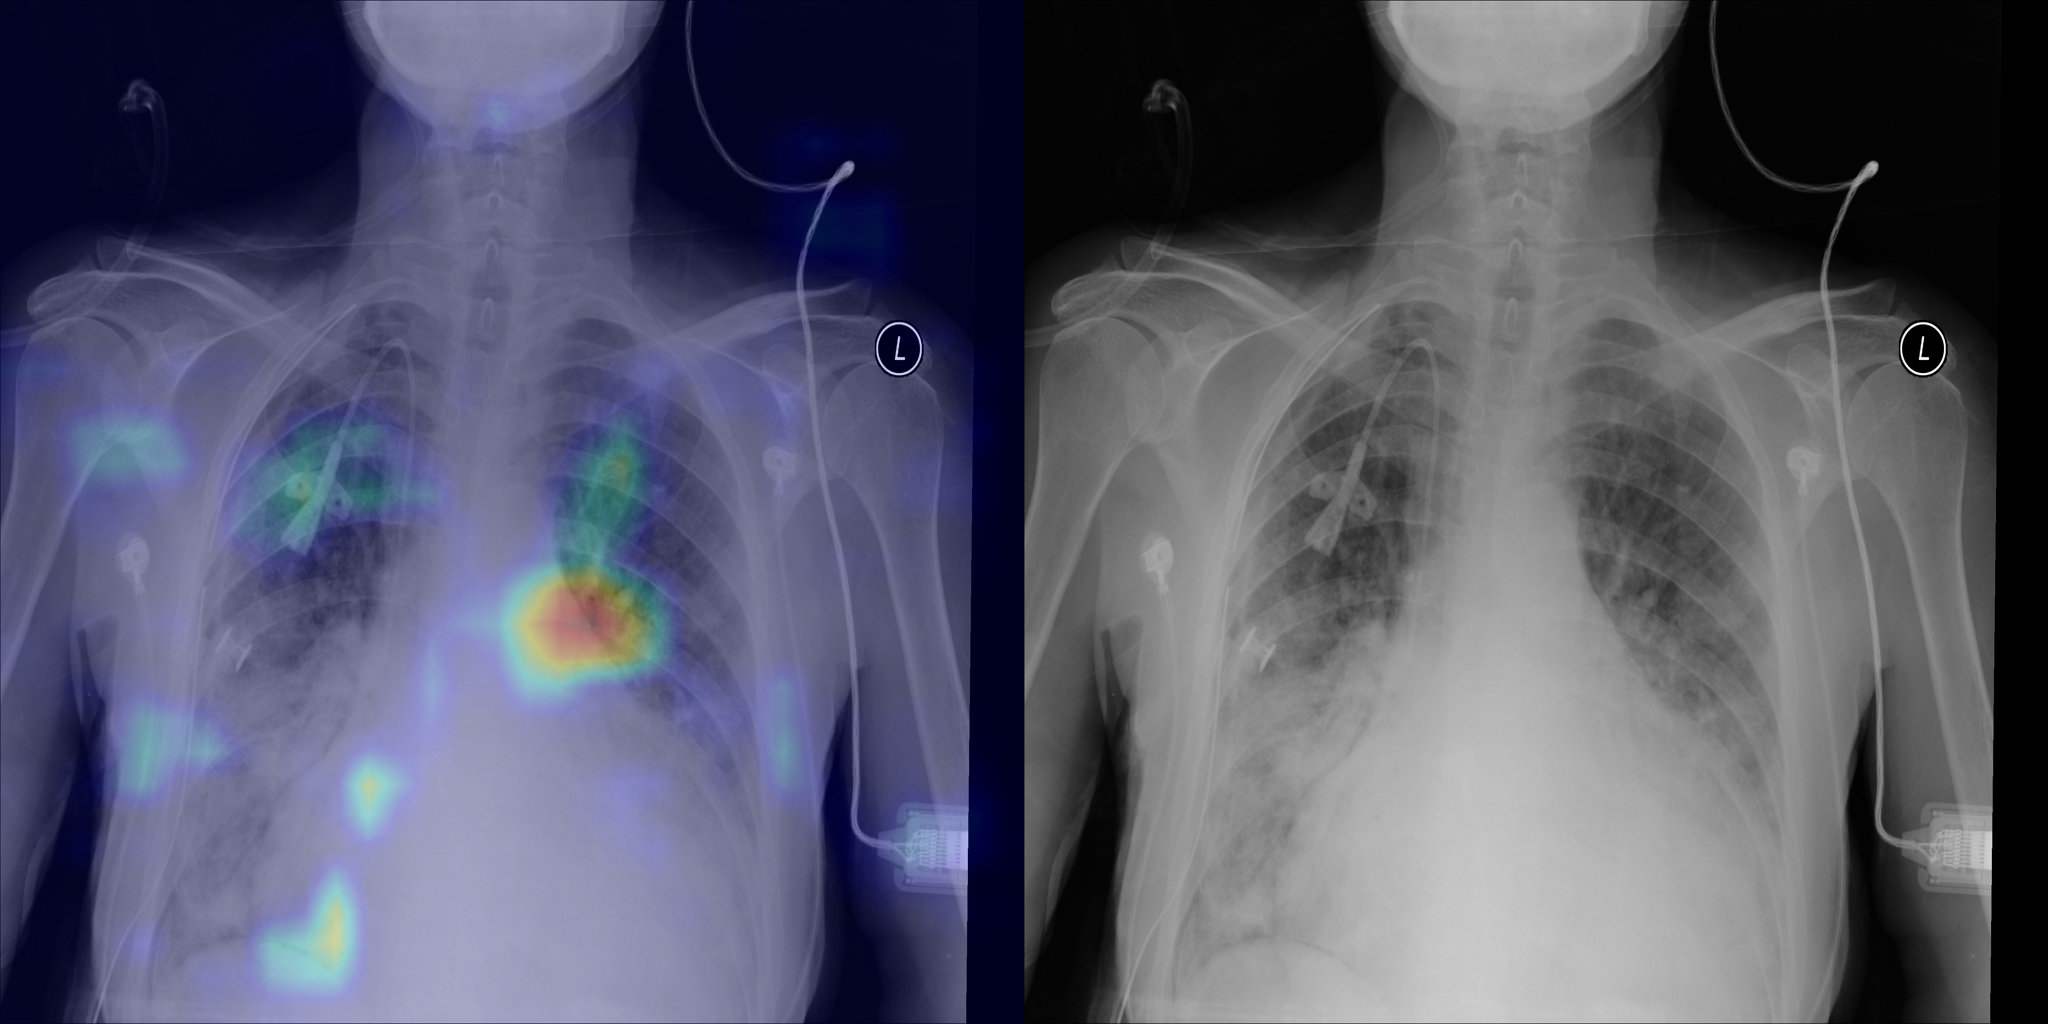
\includegraphics[width=1.0\textwidth]{Chapters/5. Conclusiones/img/Cardiomegaly/1_0_00000211_018.png}
    \end{subfigure}
    \begin{subfigure}{0.4\textwidth}
        \centering
        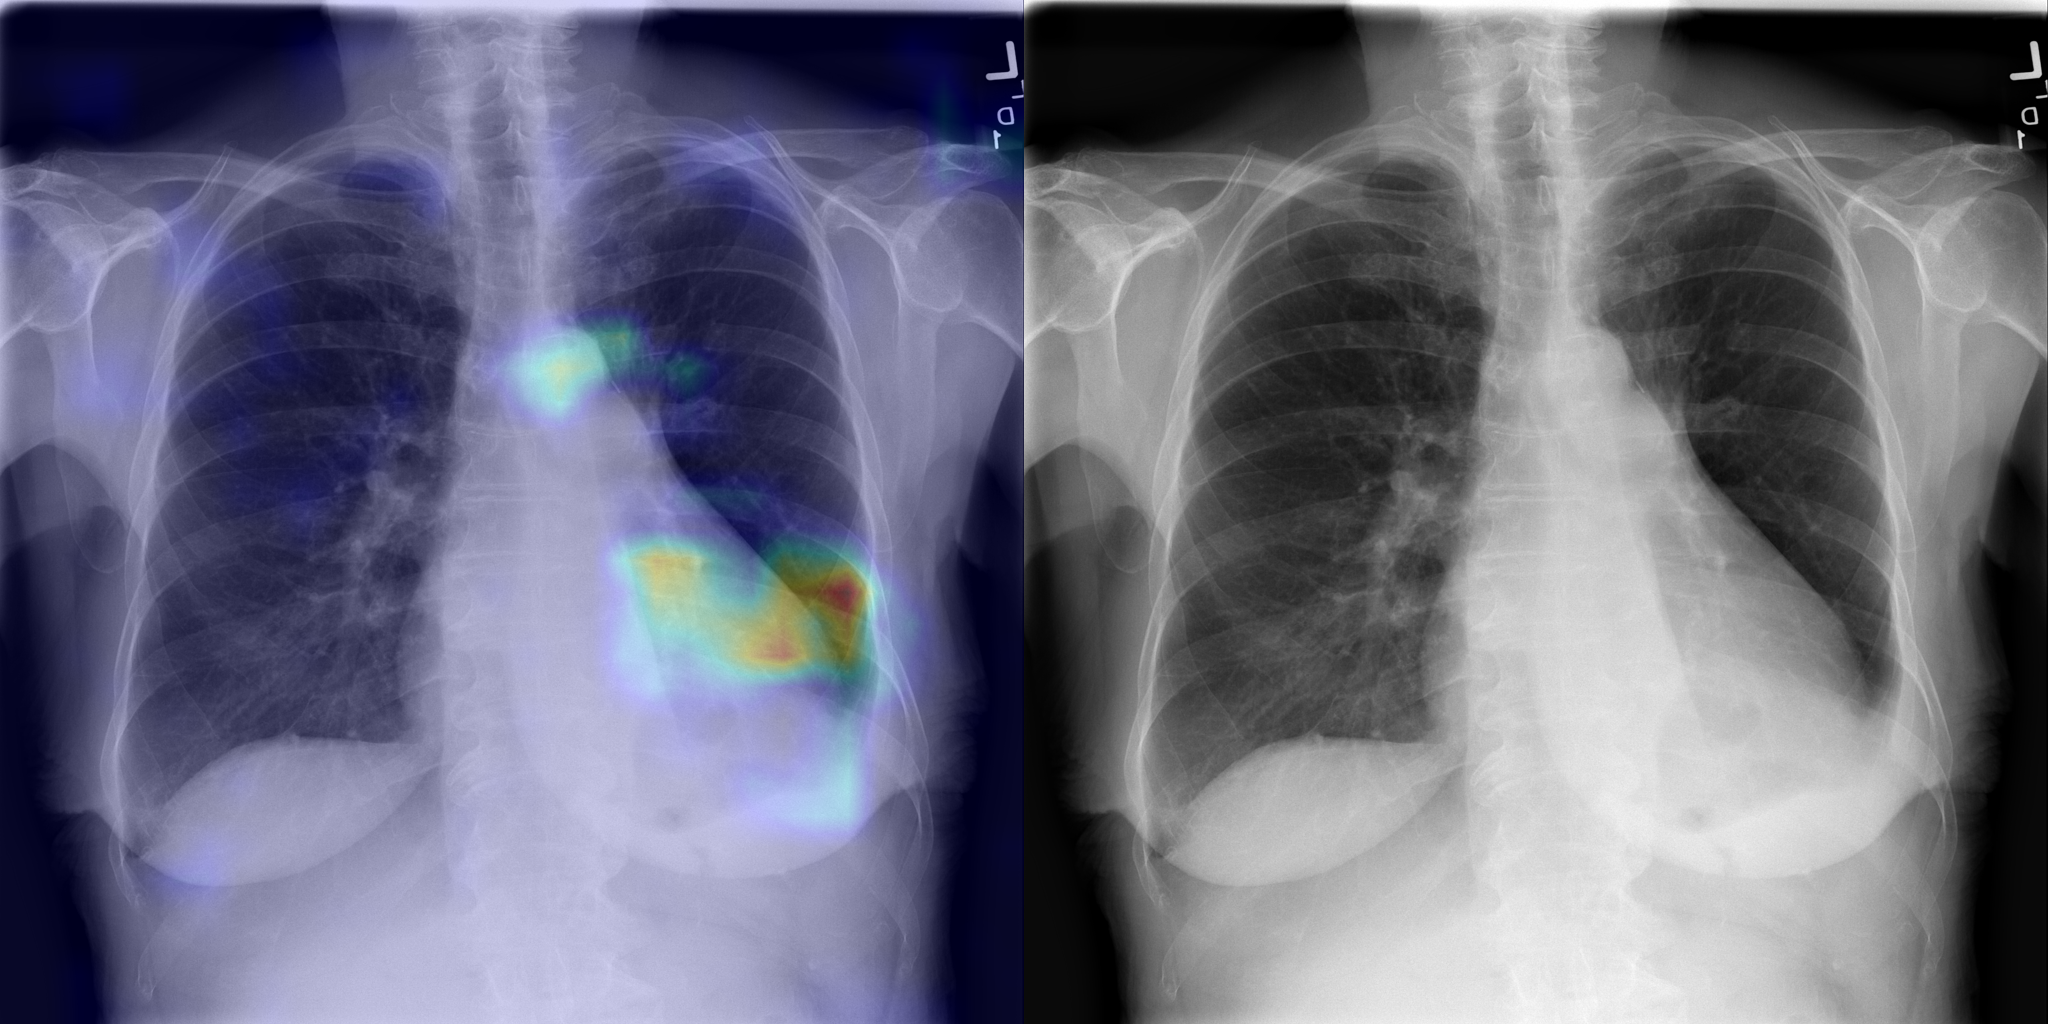
\includegraphics[width=1.0\textwidth]{Chapters/5. Conclusiones/img/Cardiomegaly/1_0_00000732_008.png}
    \end{subfigure}
    \begin{subfigure}{0.4\textwidth}
        \centering
        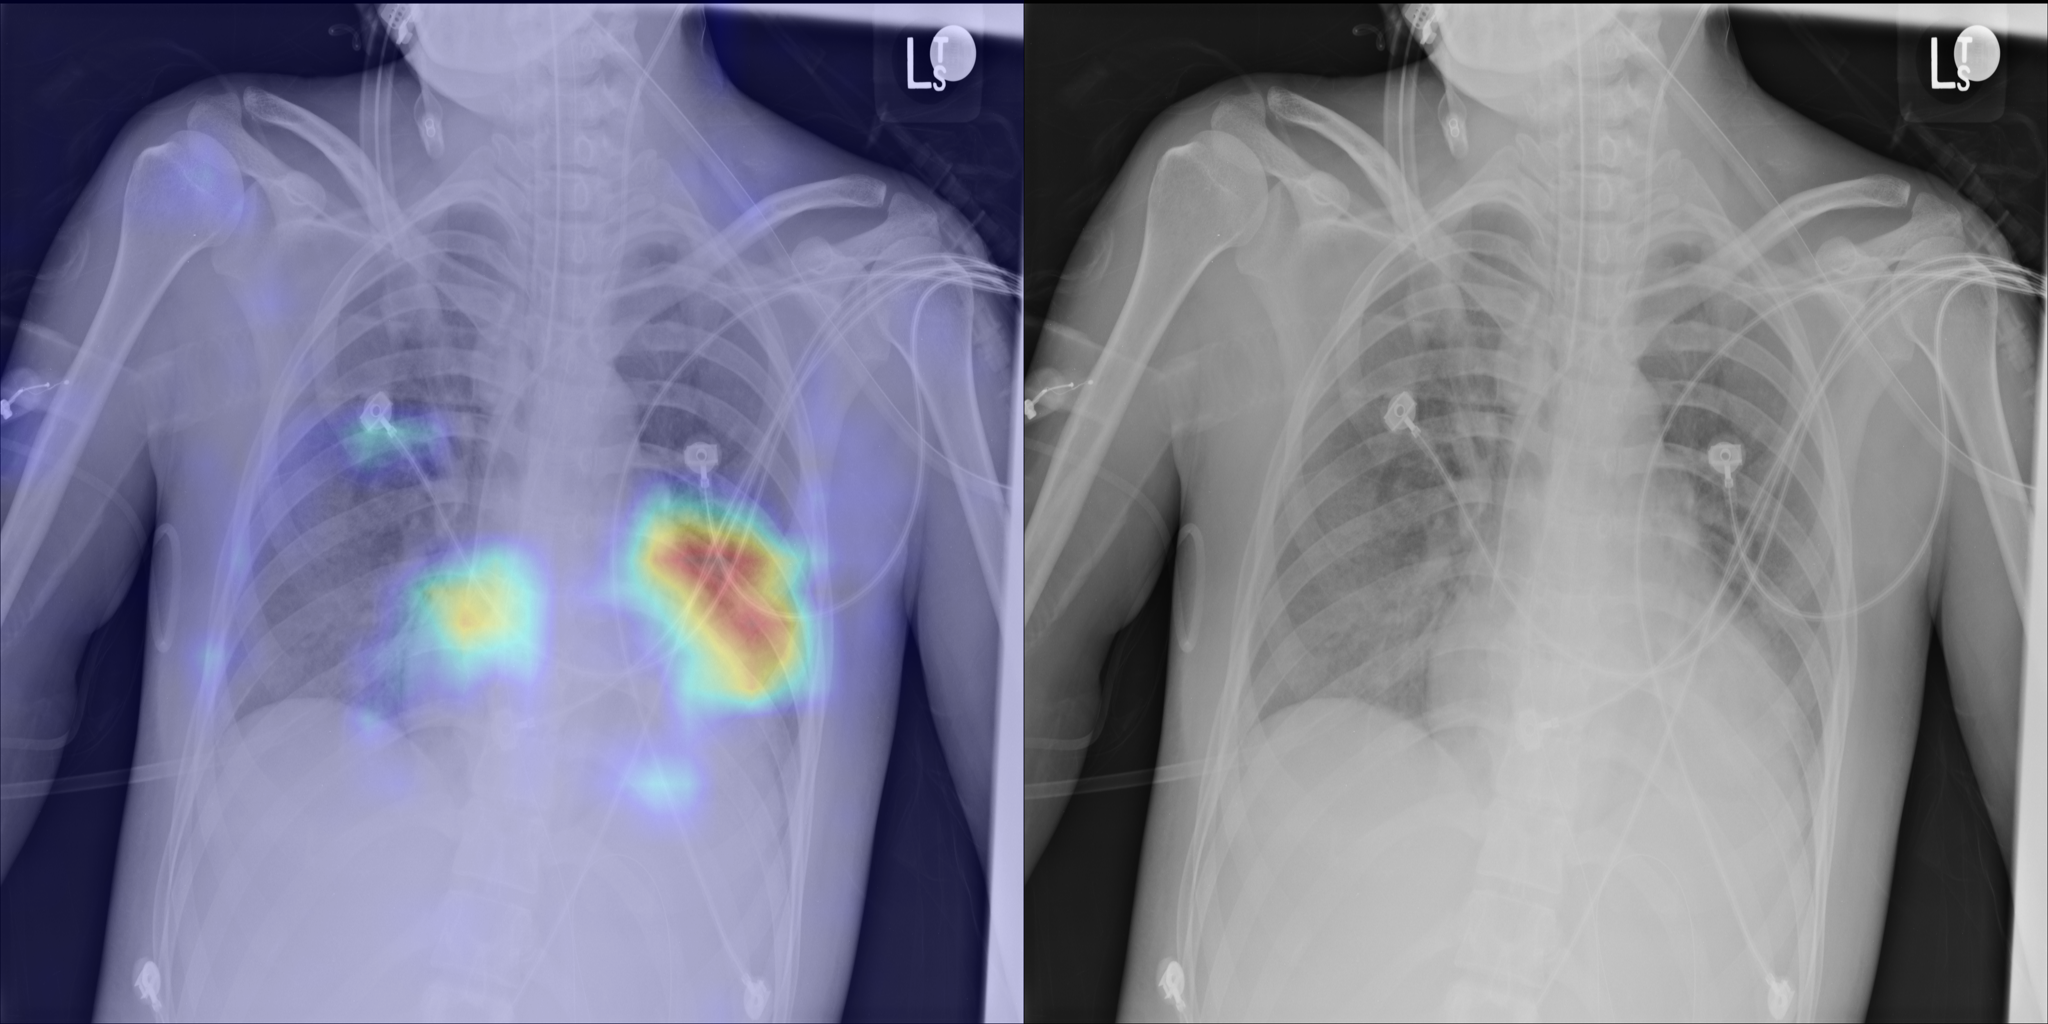
\includegraphics[width=1.0\textwidth]{Chapters/5. Conclusiones/img/Cardiomegaly/1_0_00001582_008.png}
    \end{subfigure}
    \begin{subfigure}{0.4\textwidth}
        \centering
        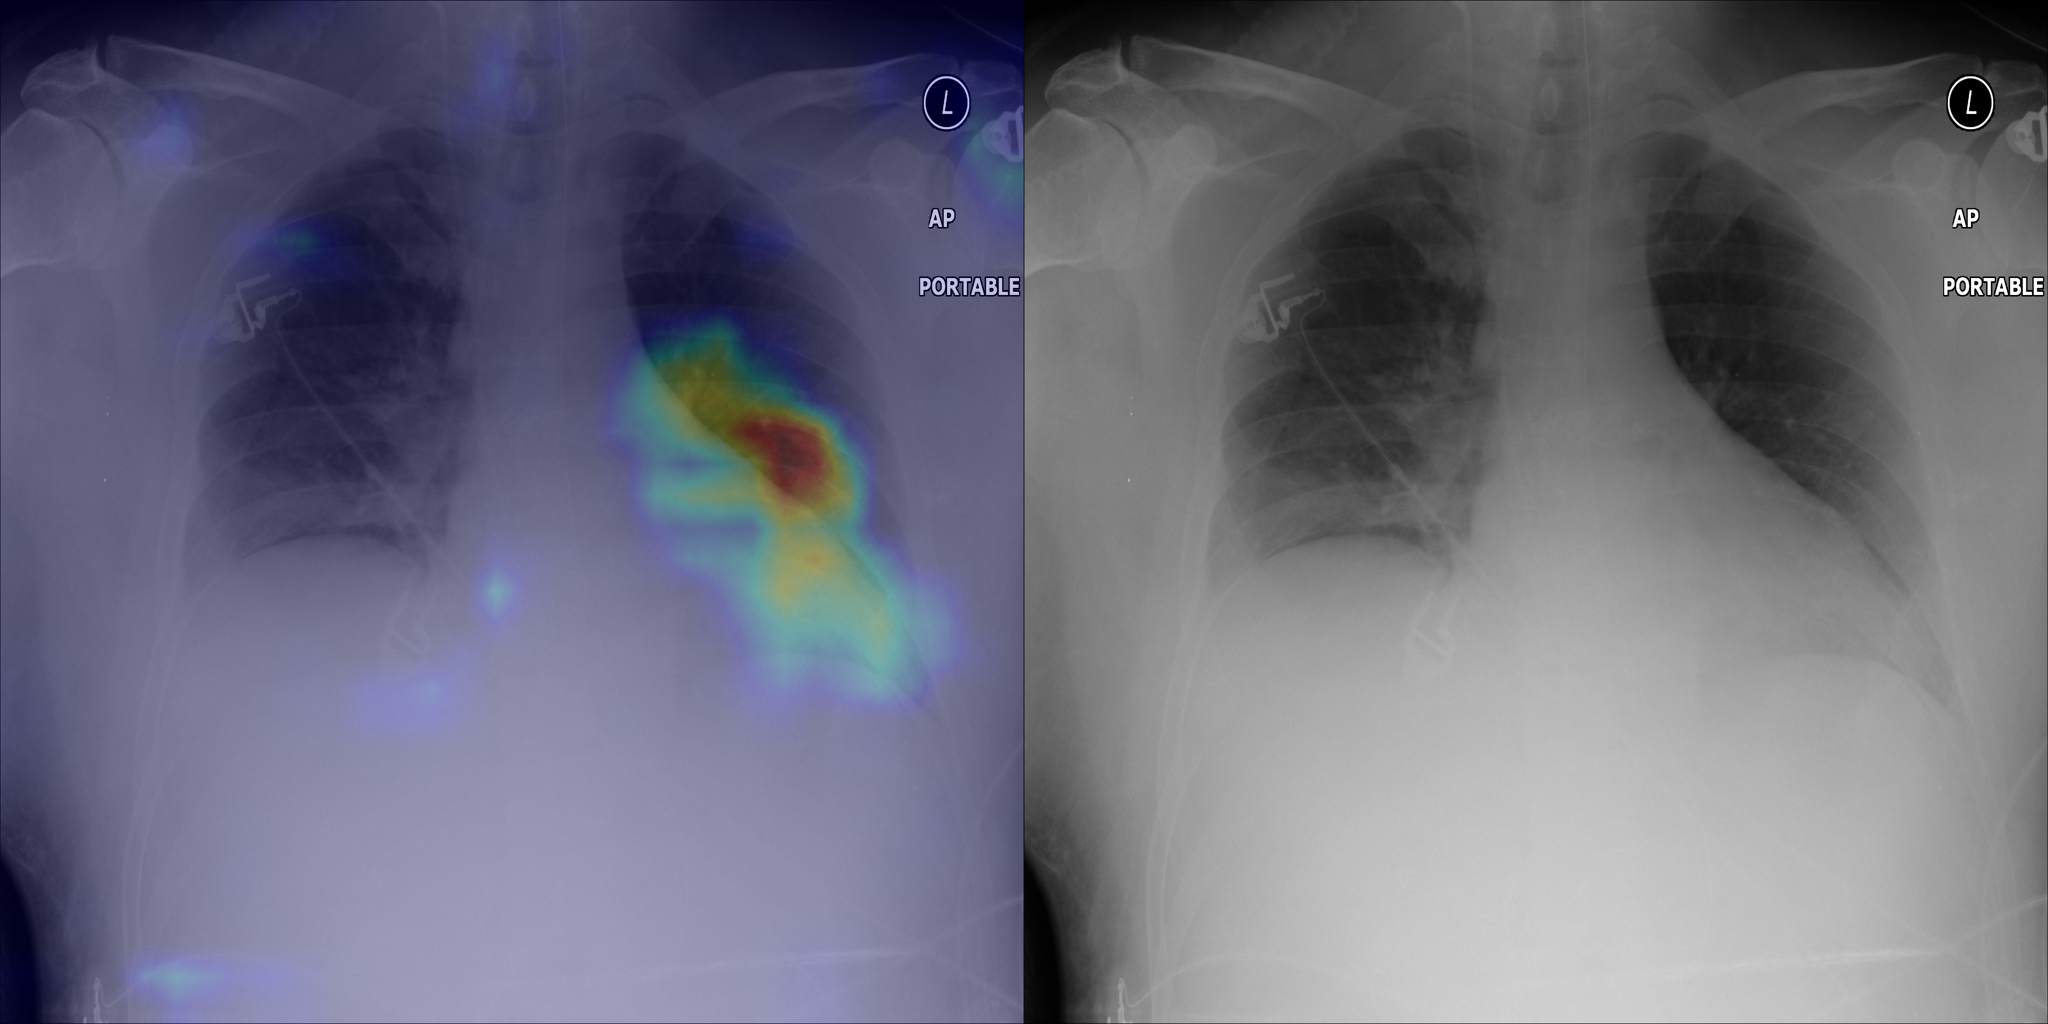
\includegraphics[width=1.0\textwidth]{Chapters/5. Conclusiones/img/Cardiomegaly/1_0_00002059_002.png}
    \end{subfigure}
    \begin{subfigure}{0.4\textwidth}
        \centering
        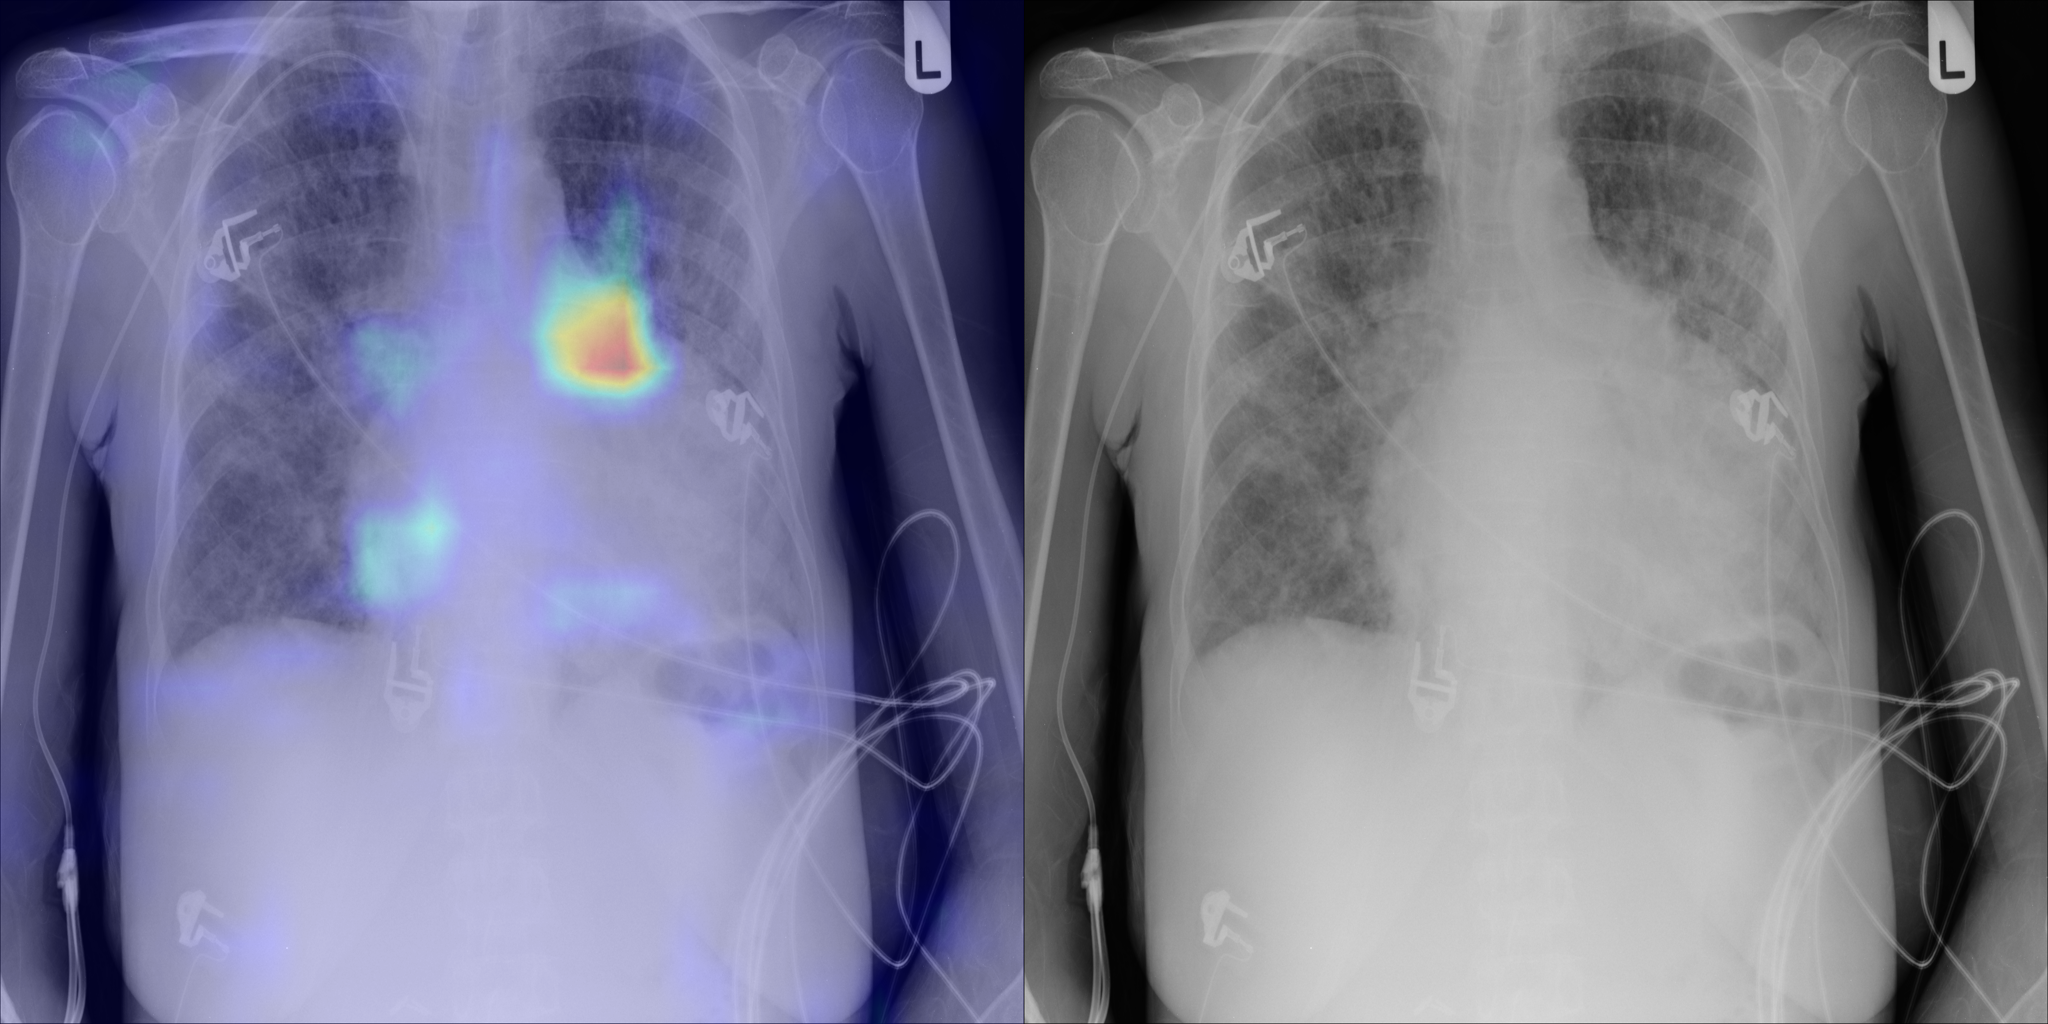
\includegraphics[width=1.0\textwidth]{Chapters/5. Conclusiones/img/Cardiomegaly/1_0_00004344_039.png}
    \end{subfigure}
    \begin{subfigure}{0.4\textwidth}
        \centering
        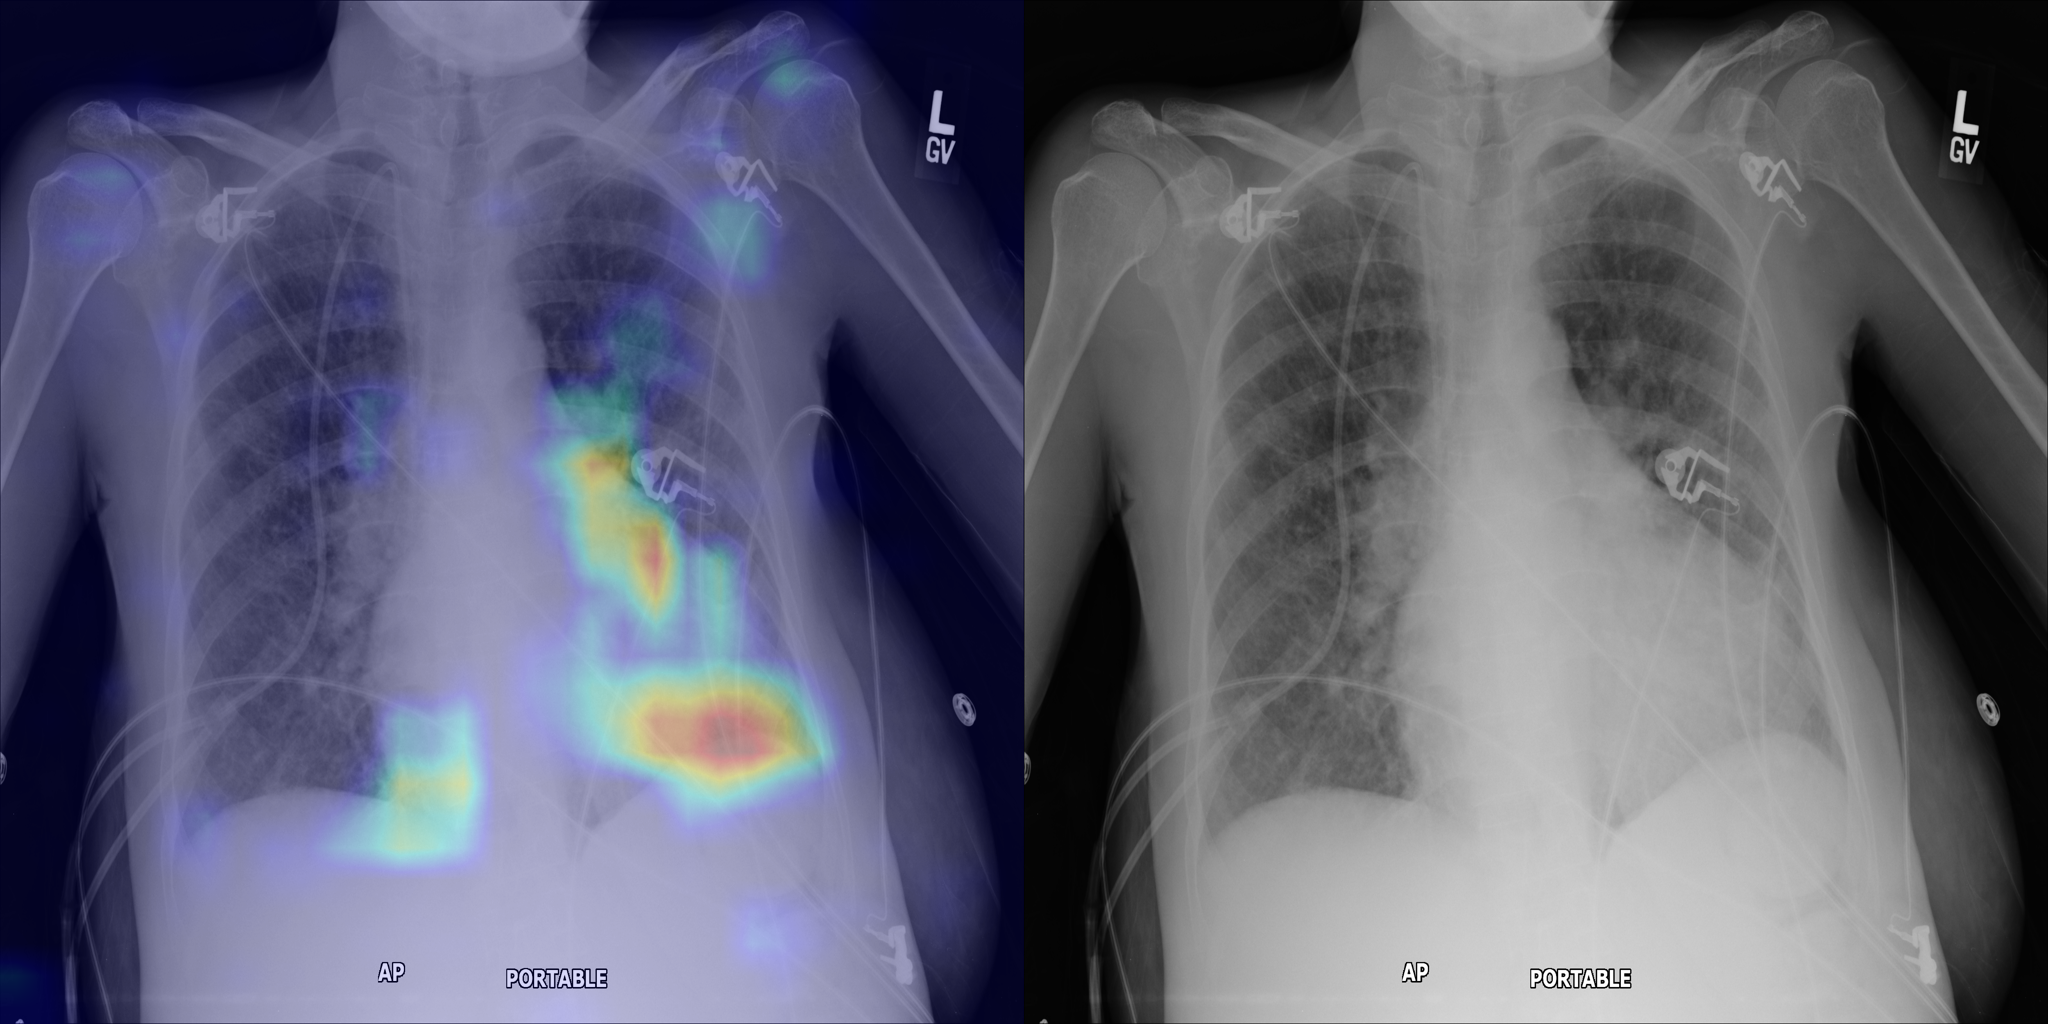
\includegraphics[width=1.0\textwidth]{Chapters/5. Conclusiones/img/Cardiomegaly/1_0_00004344_045.png}
    \end{subfigure}
    \begin{subfigure}{0.4\textwidth}
        \centering
        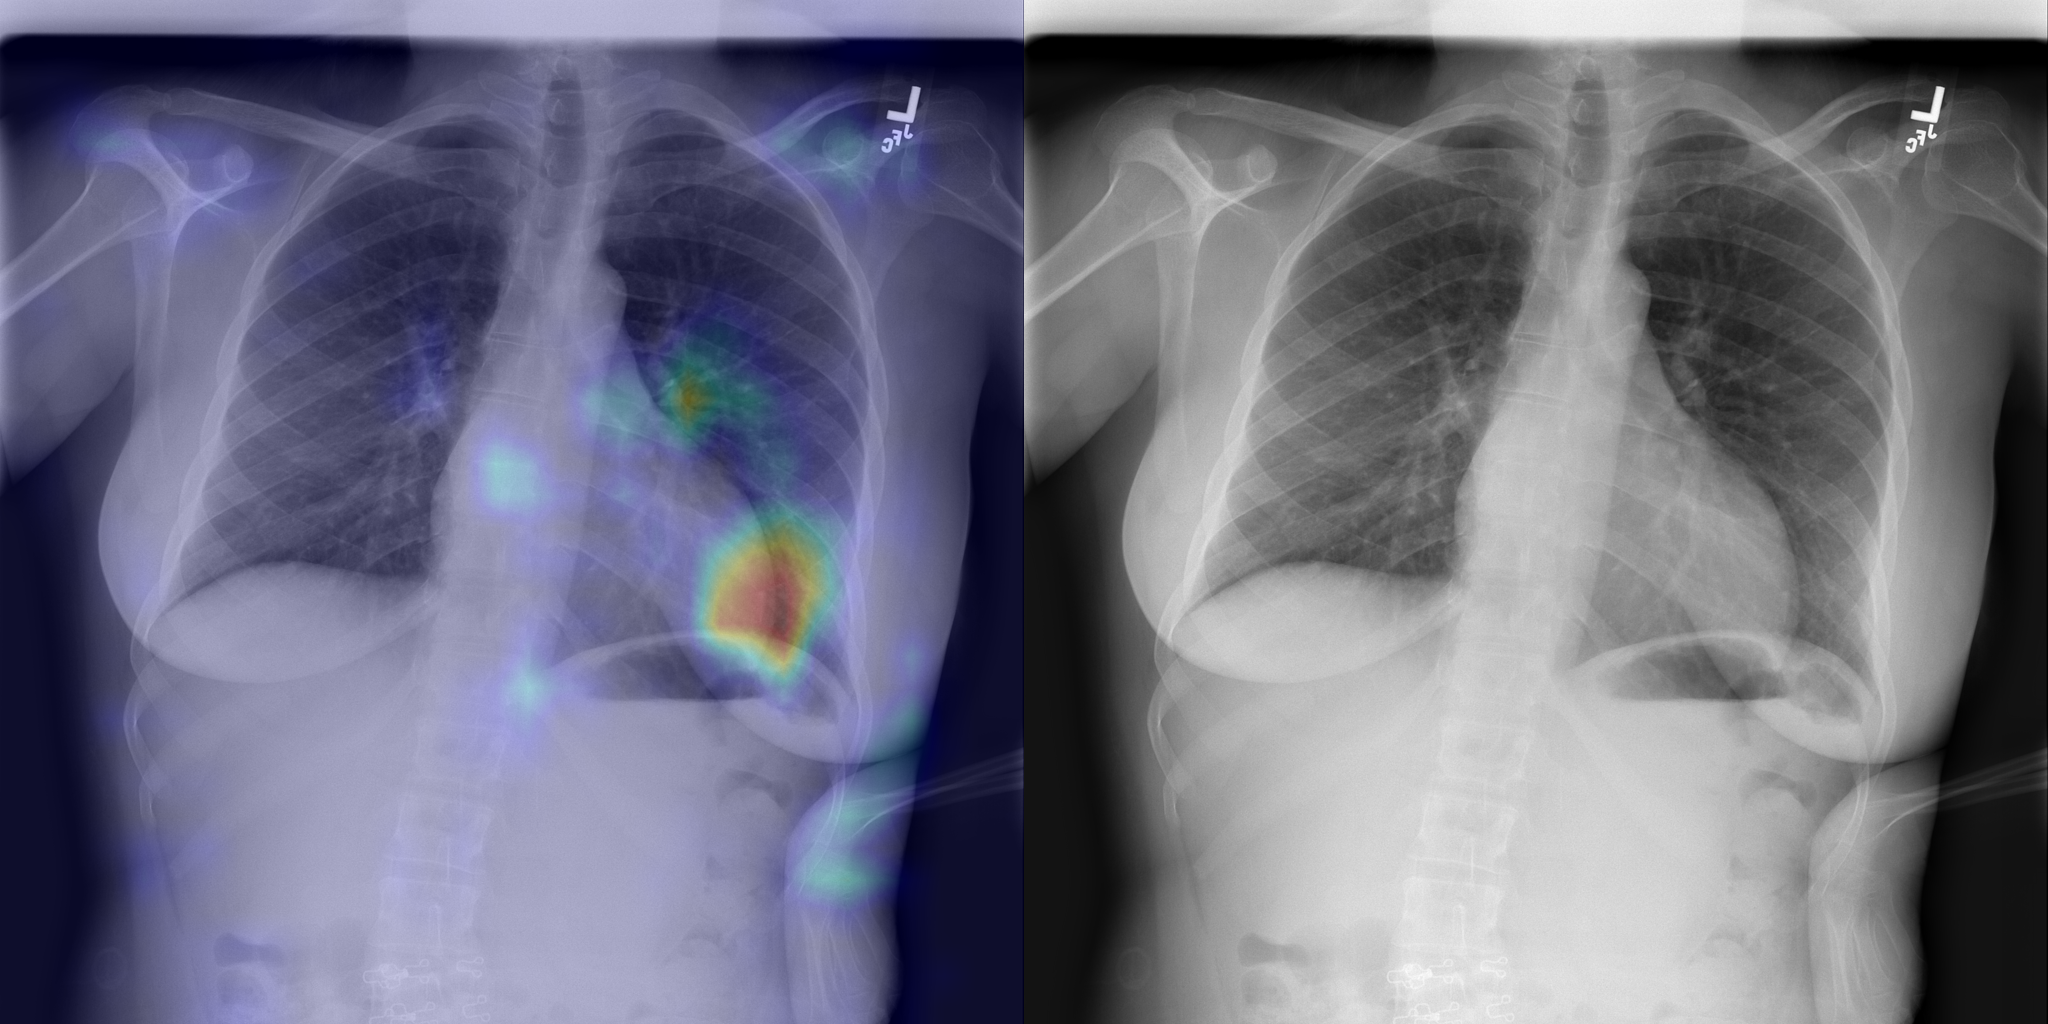
\includegraphics[width=1.0\textwidth]{Chapters/5. Conclusiones/img/Cardiomegaly/1_0_00004526_017.png}
    \end{subfigure}
    \begin{subfigure}{0.4\textwidth}
        \centering
        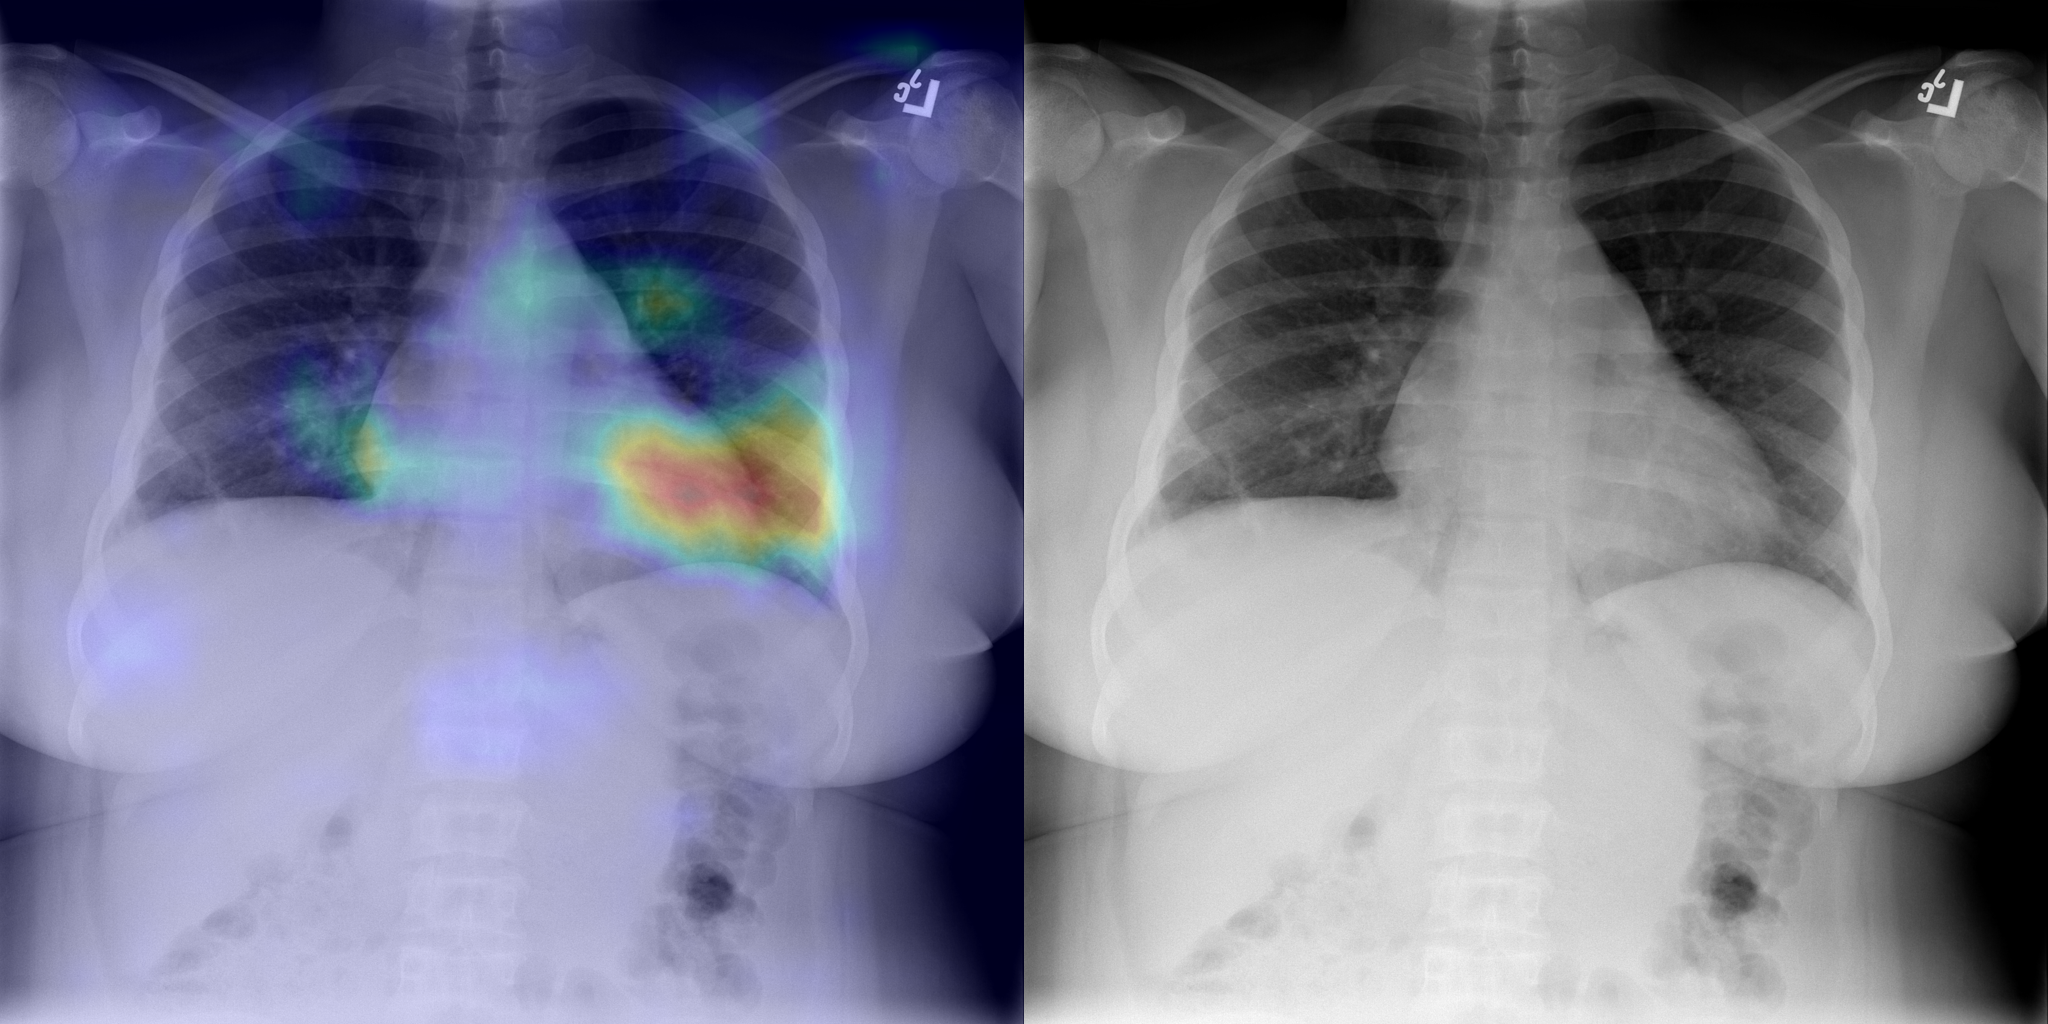
\includegraphics[width=1.0\textwidth]{Chapters/5. Conclusiones/img/Cardiomegaly/1_1_00014706_010.png}
    \end{subfigure}
    \begin{subfigure}{0.4\textwidth}
        \centering
        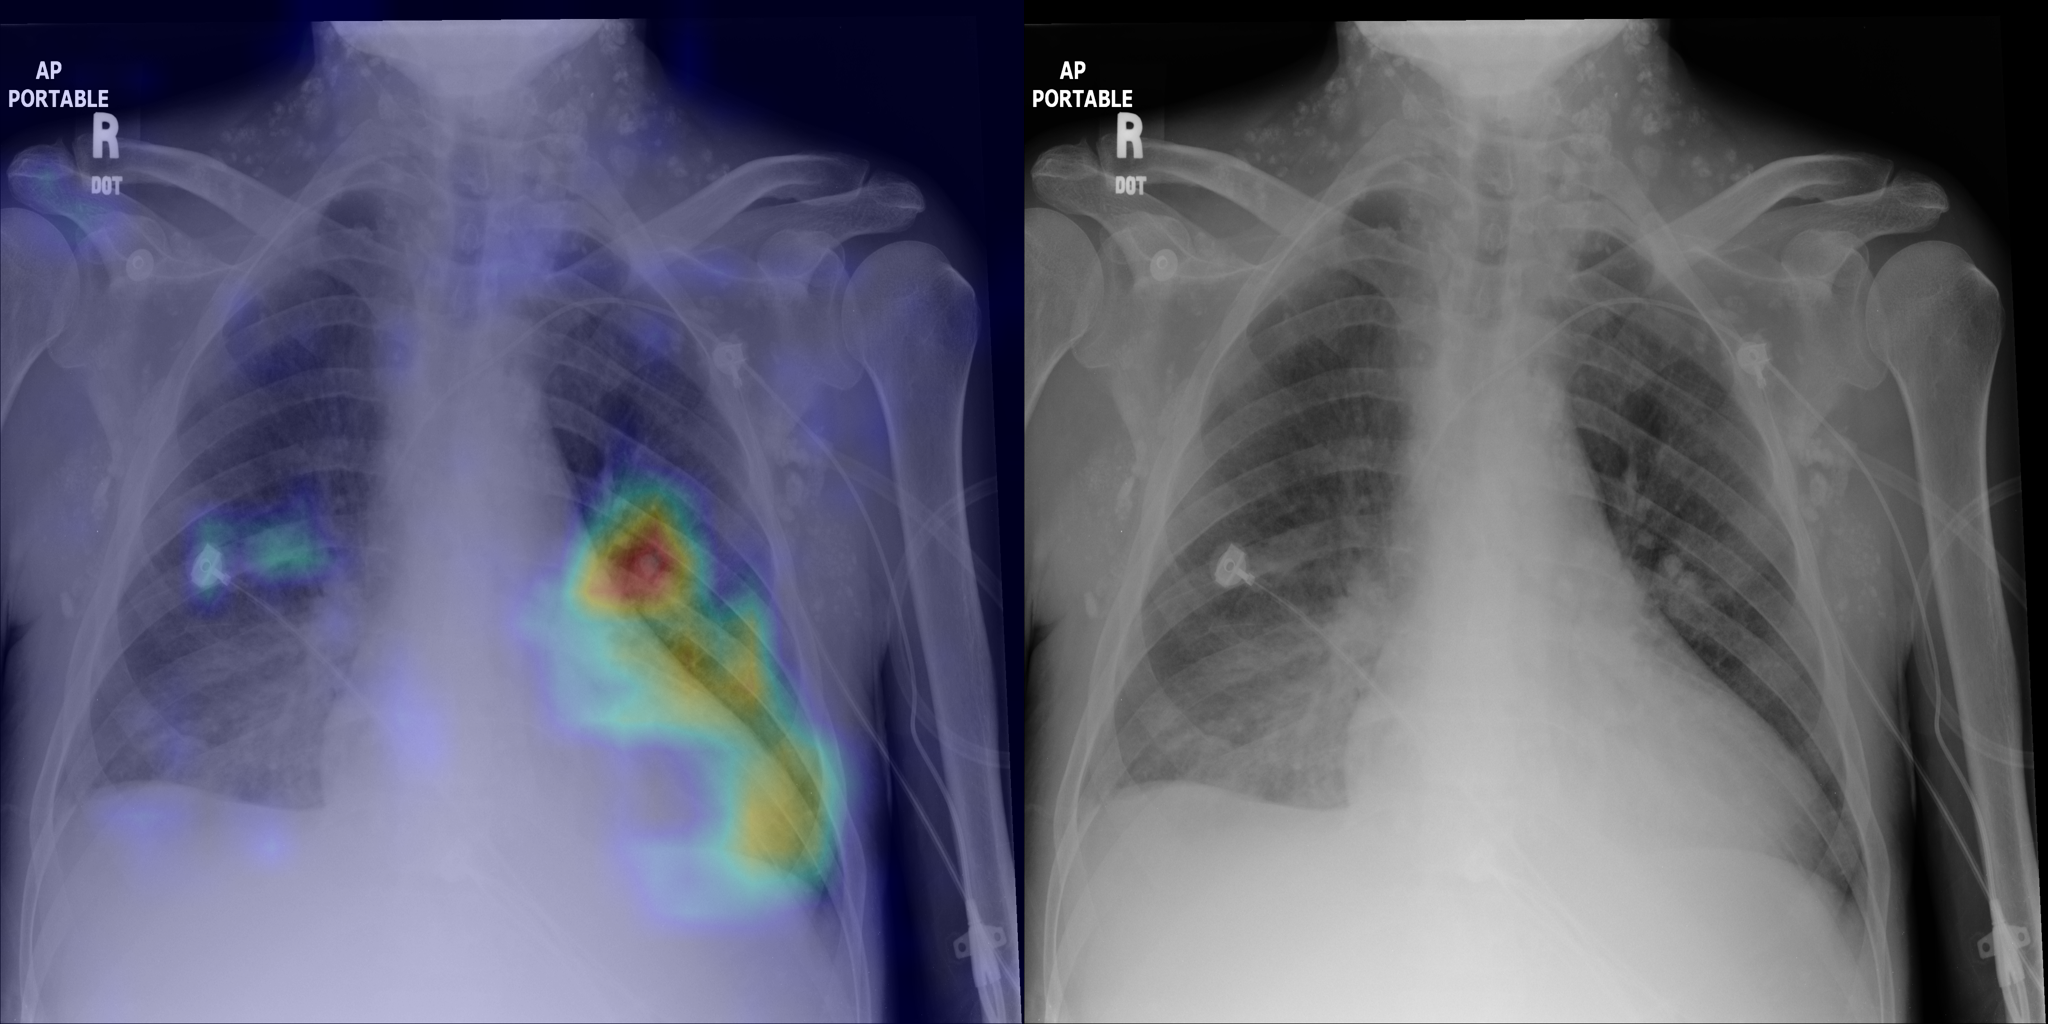
\includegraphics[width=1.0\textwidth]{Chapters/5. Conclusiones/img/Cardiomegaly/1_1_00016291_042.png}
    \end{subfigure}

    \caption{Cardiomegalia. Radiografías detectadas con la patología de cardiomegalia por los
                    radiólogos. A la izquierda de cada imagen el GradCam correspondiente a la detección
                    de la patología como positivo por el modelo CNN.}

    \label{fig-cardiomegalia}
\end{figure}

\begin{figure}[b]
    \centering
    \begin{subfigure}{0.4\textwidth}
        \centering
        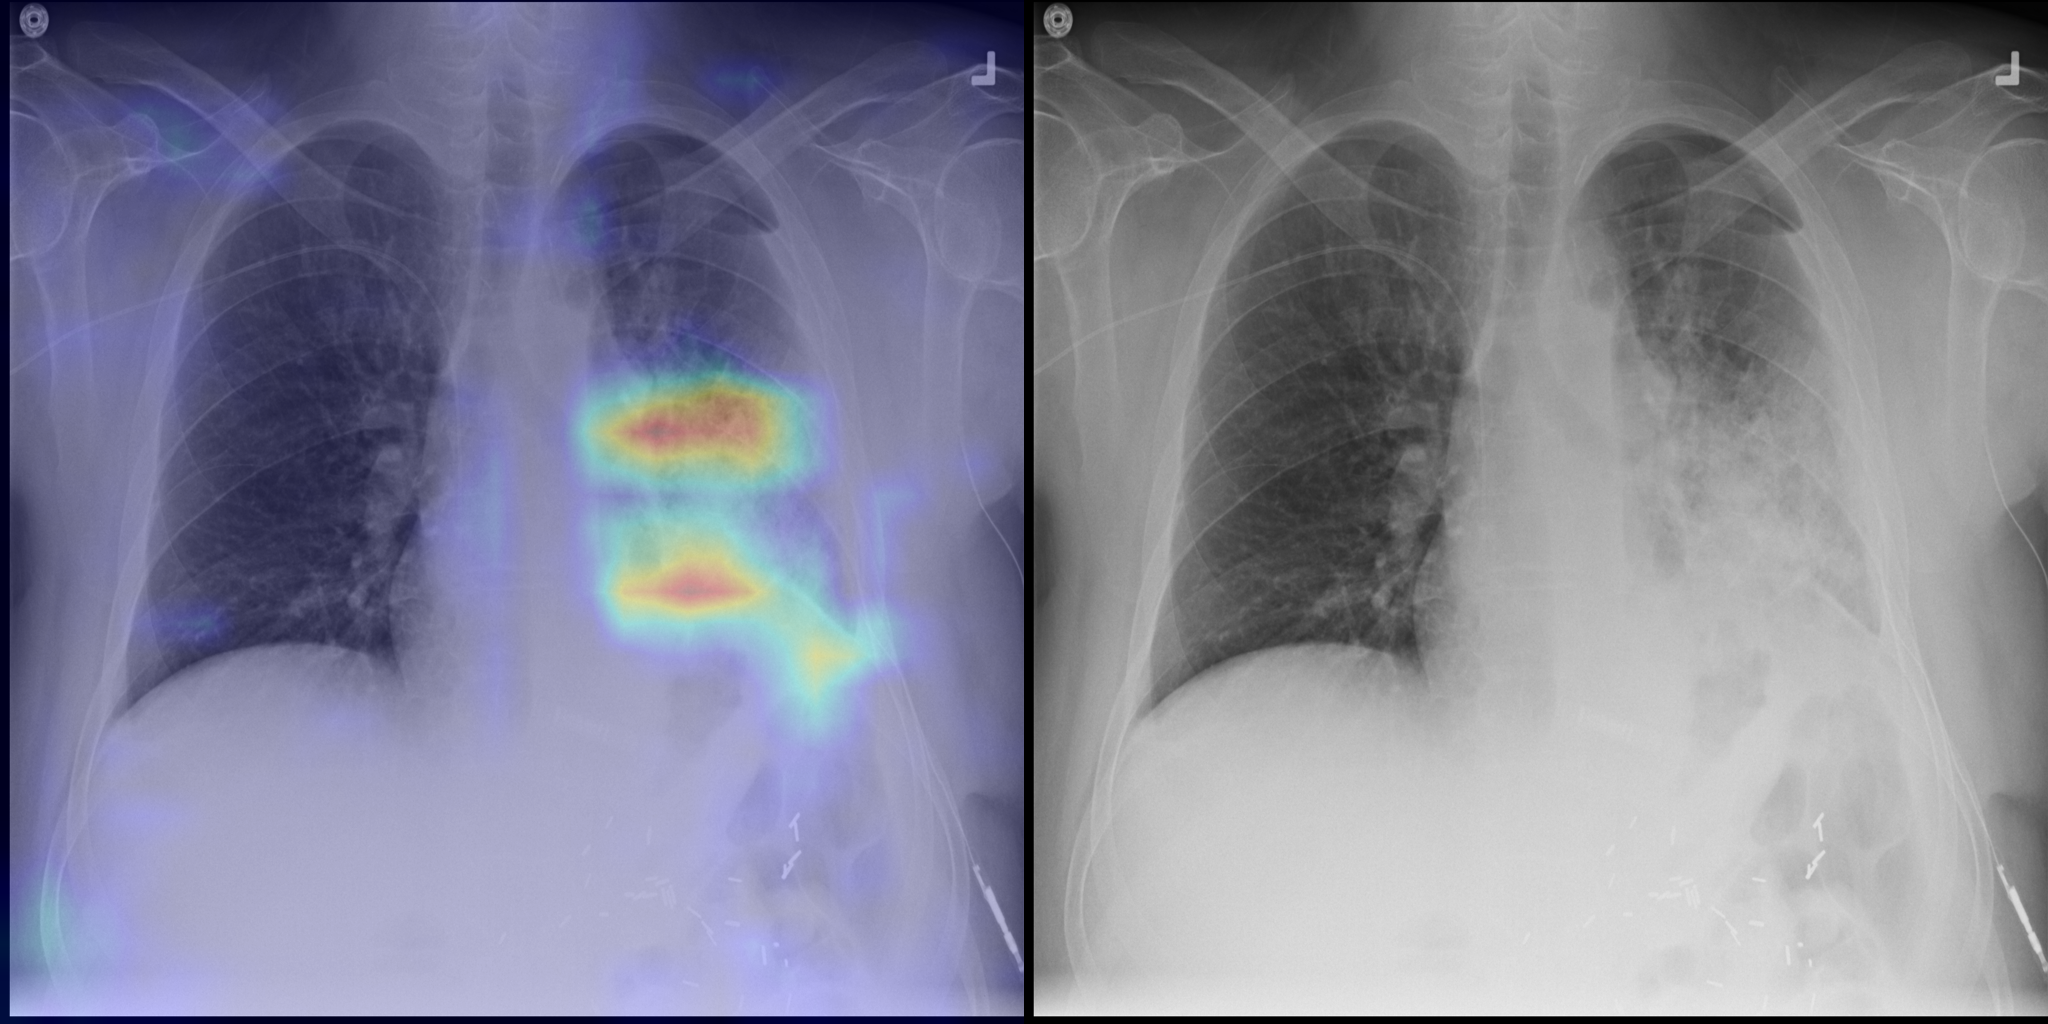
\includegraphics[width=1.0\textwidth]{Chapters/5. Conclusiones/img/Consolidation/1_1_00000246_014.png}
    \end{subfigure}
    \begin{subfigure}{0.4\textwidth}
        \centering
        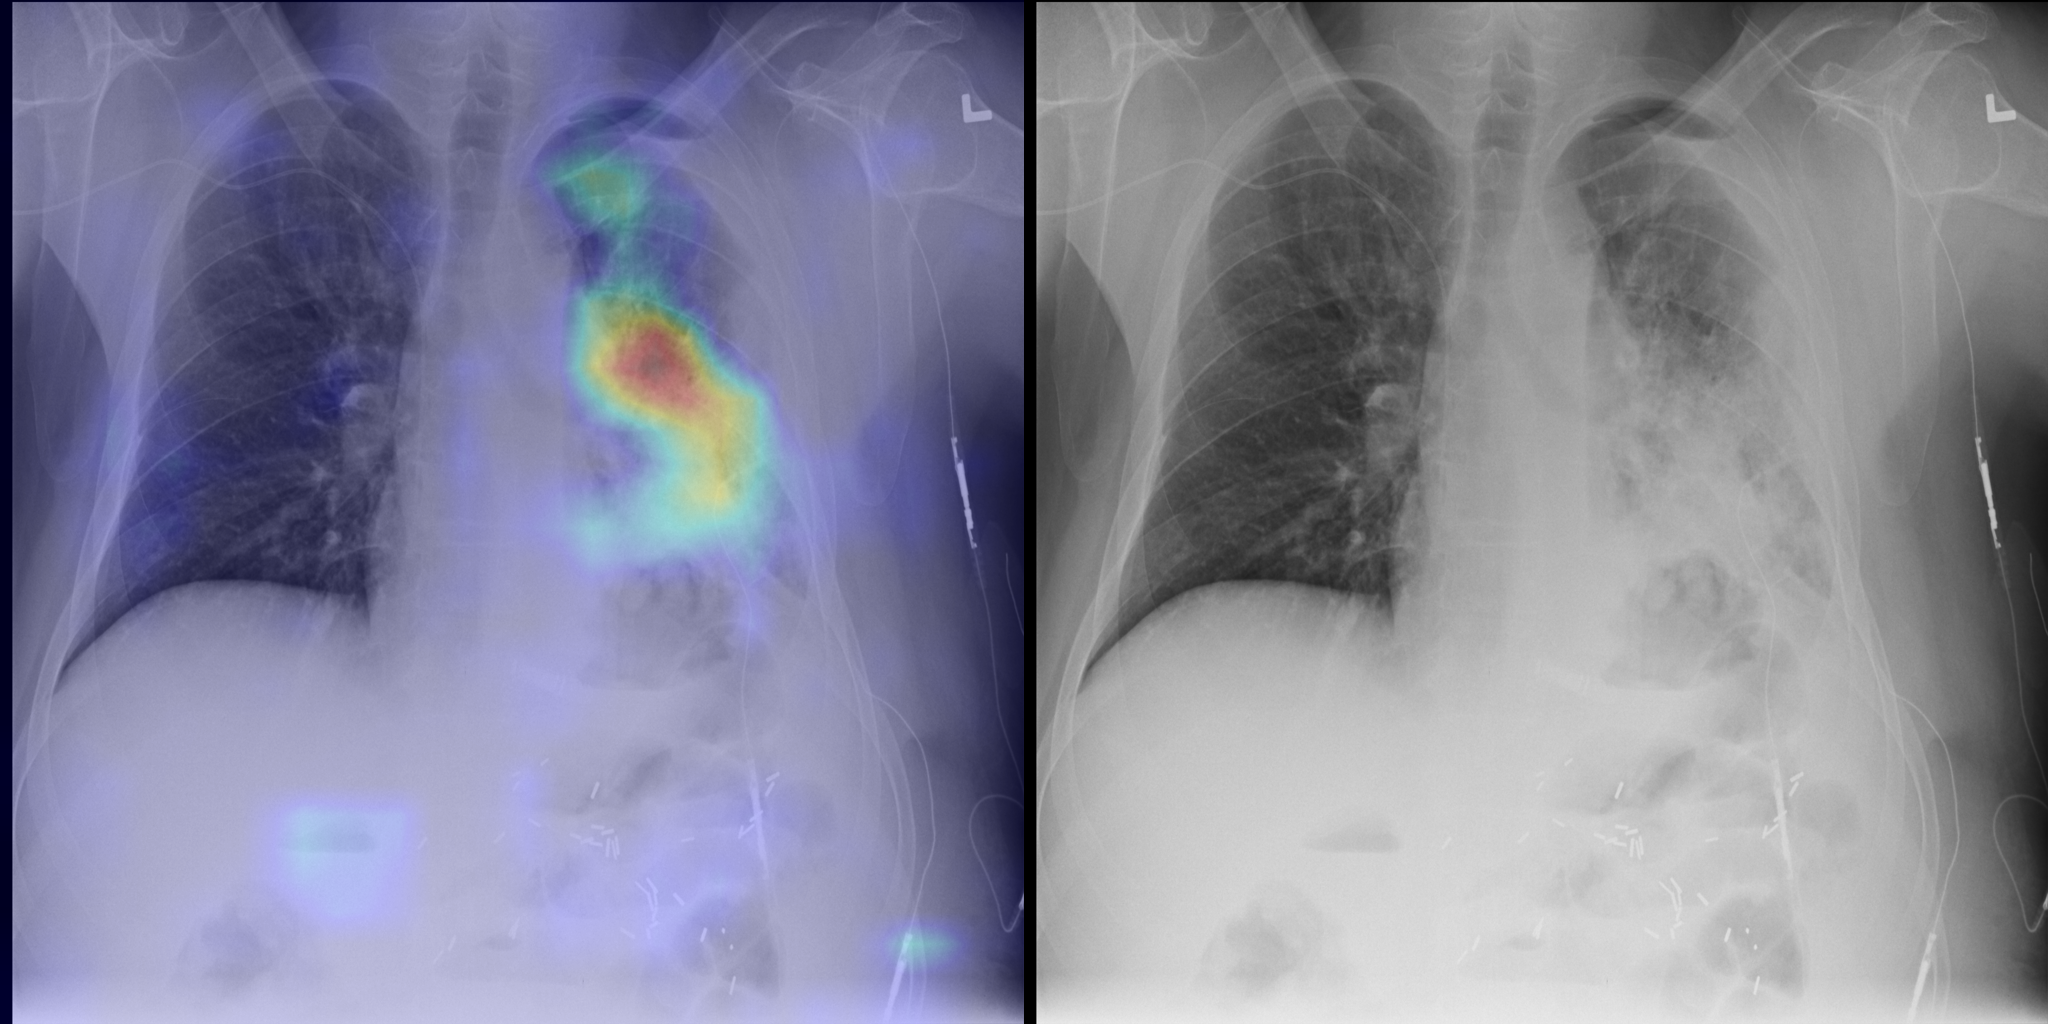
\includegraphics[width=1.0\textwidth]{Chapters/5. Conclusiones/img/Consolidation/1_1_00000246_016.png}
    \end{subfigure}
    \begin{subfigure}{0.4\textwidth}
        \centering
        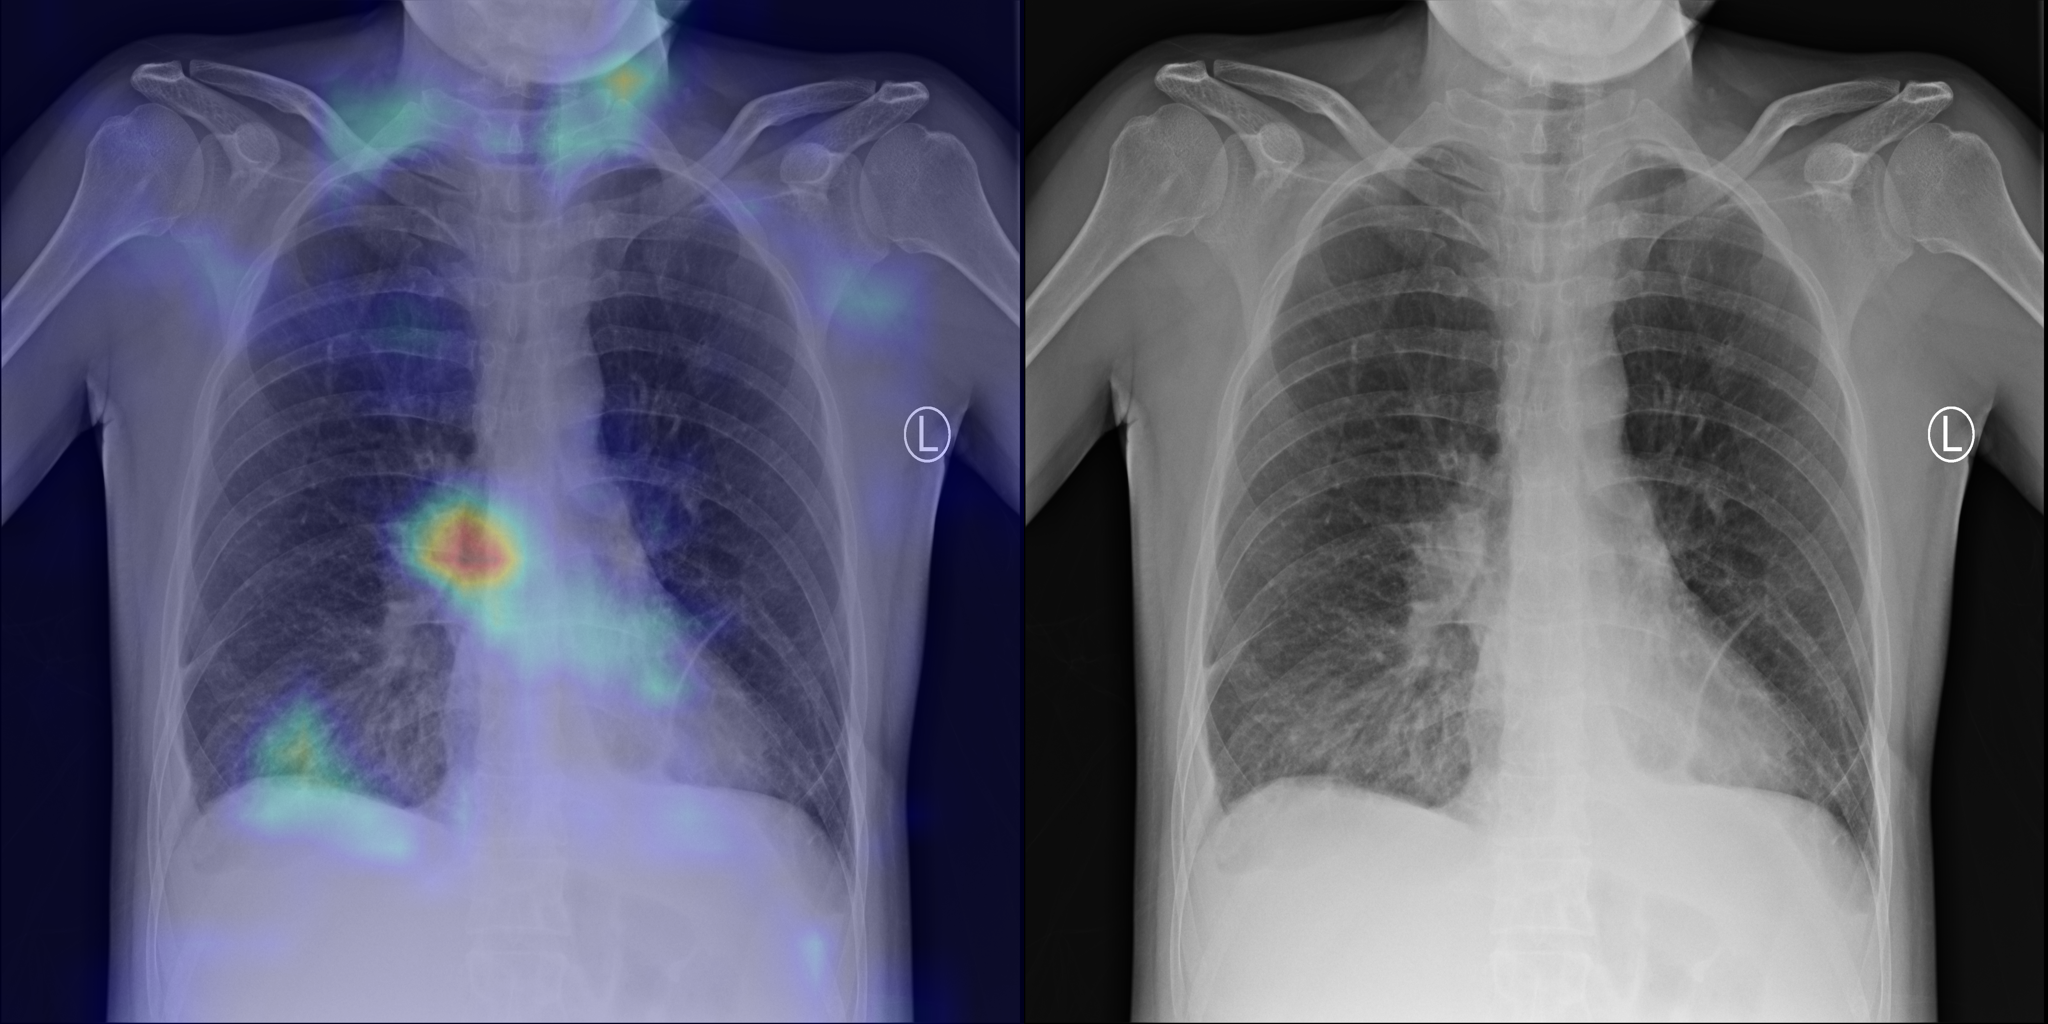
\includegraphics[width=1.0\textwidth]{Chapters/5. Conclusiones/img/Consolidation/1_1_00000344_000.png}
    \end{subfigure}
    \begin{subfigure}{0.4\textwidth}
        \centering
        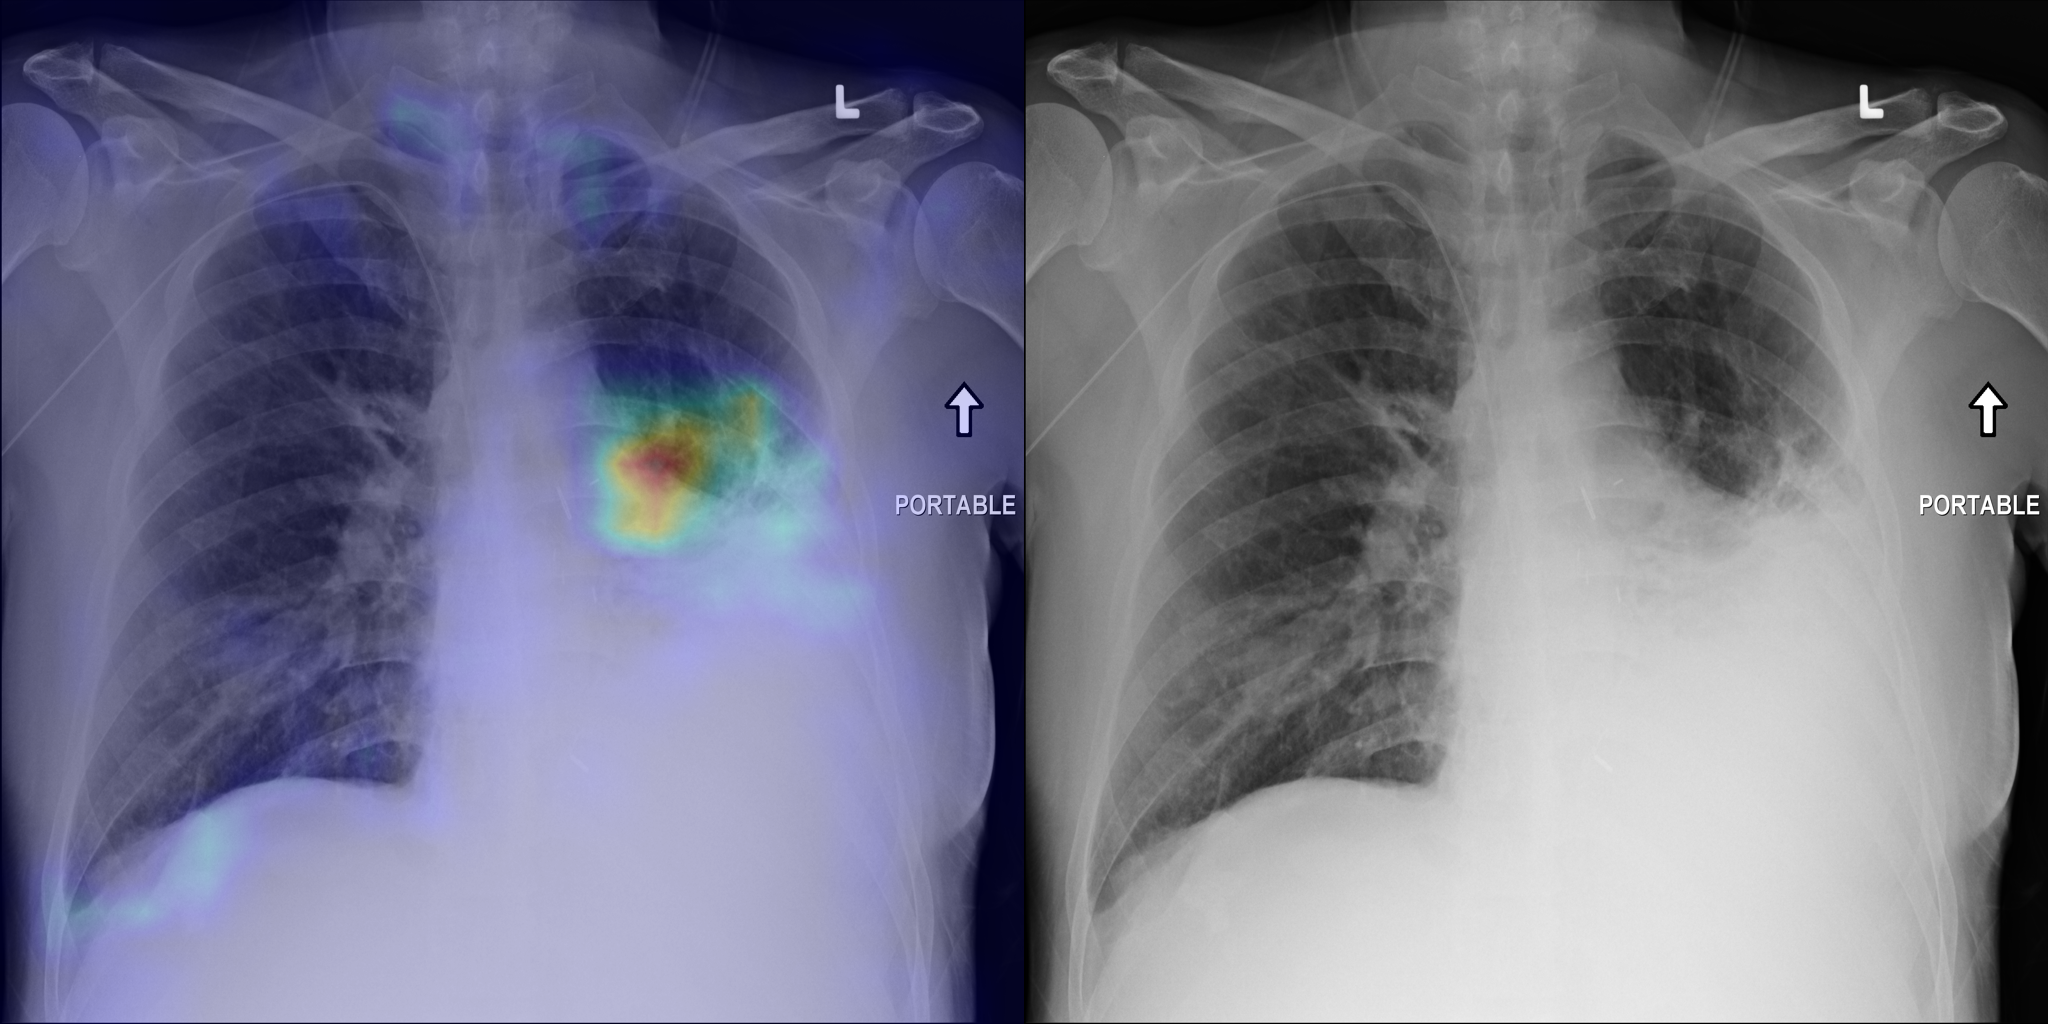
\includegraphics[width=1.0\textwidth]{Chapters/5. Conclusiones/img/Consolidation/1_1_00000467_002.png}
    \end{subfigure}
    \begin{subfigure}{0.4\textwidth}
        \centering
        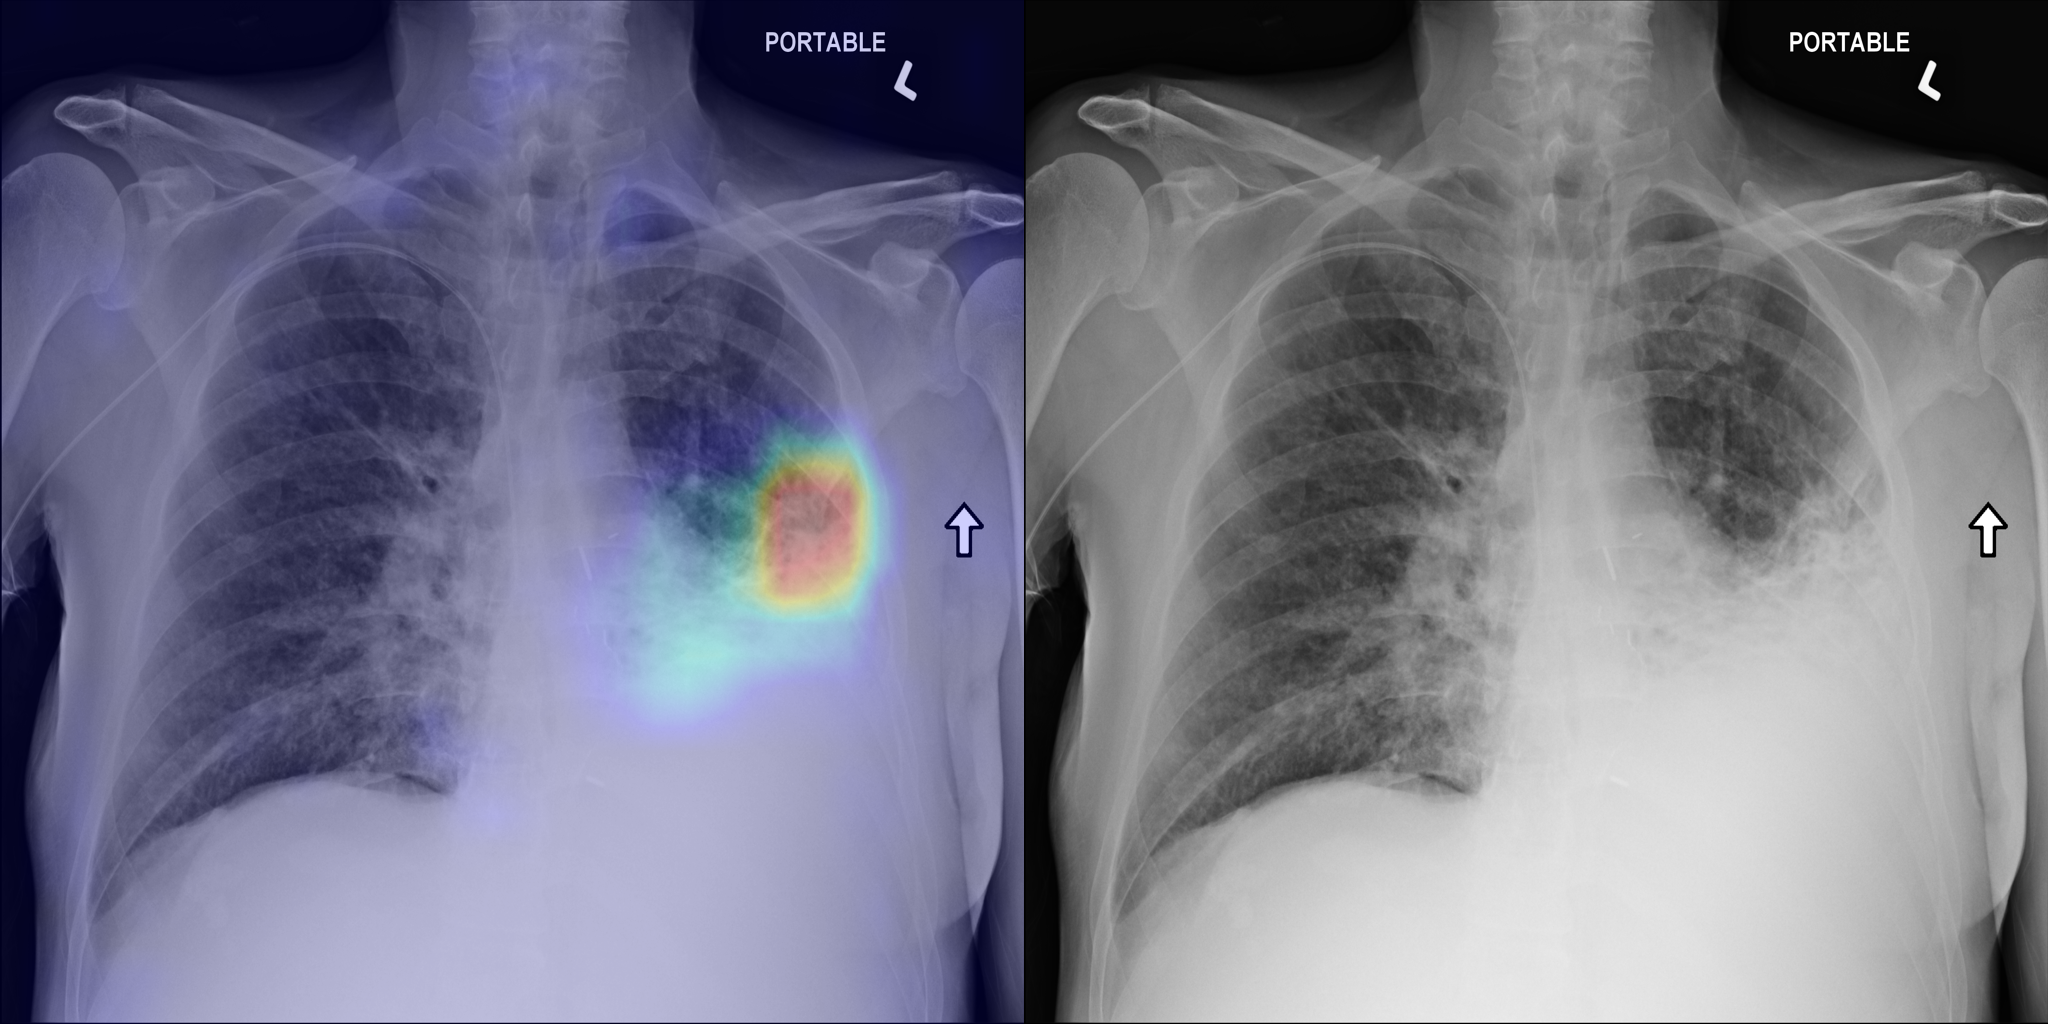
\includegraphics[width=1.0\textwidth]{Chapters/5. Conclusiones/img/Consolidation/1_1_00000467_003.png}
    \end{subfigure}
    \begin{subfigure}{0.4\textwidth}
        \centering
        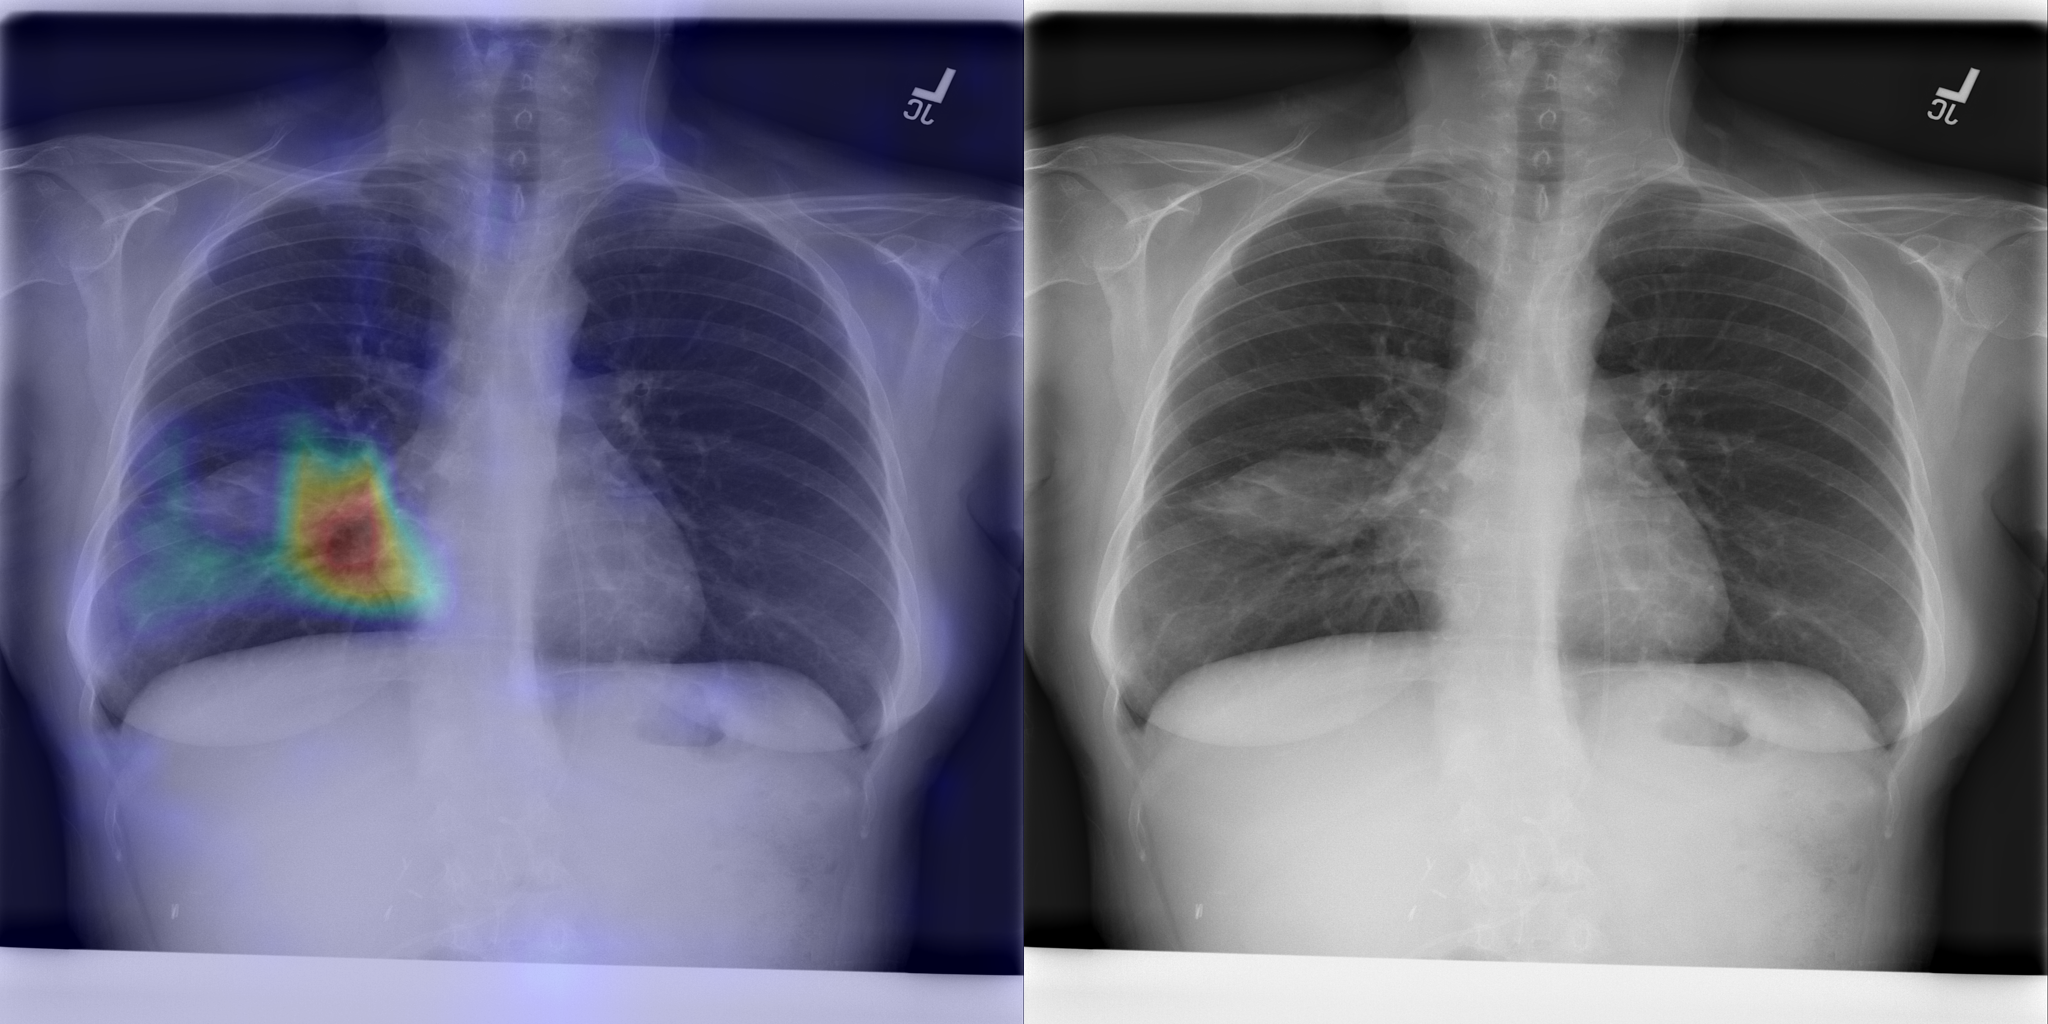
\includegraphics[width=1.0\textwidth]{Chapters/5. Conclusiones/img/Consolidation/1_1_00000618_008.png}
    \end{subfigure}
    \begin{subfigure}{0.4\textwidth}
        \centering
        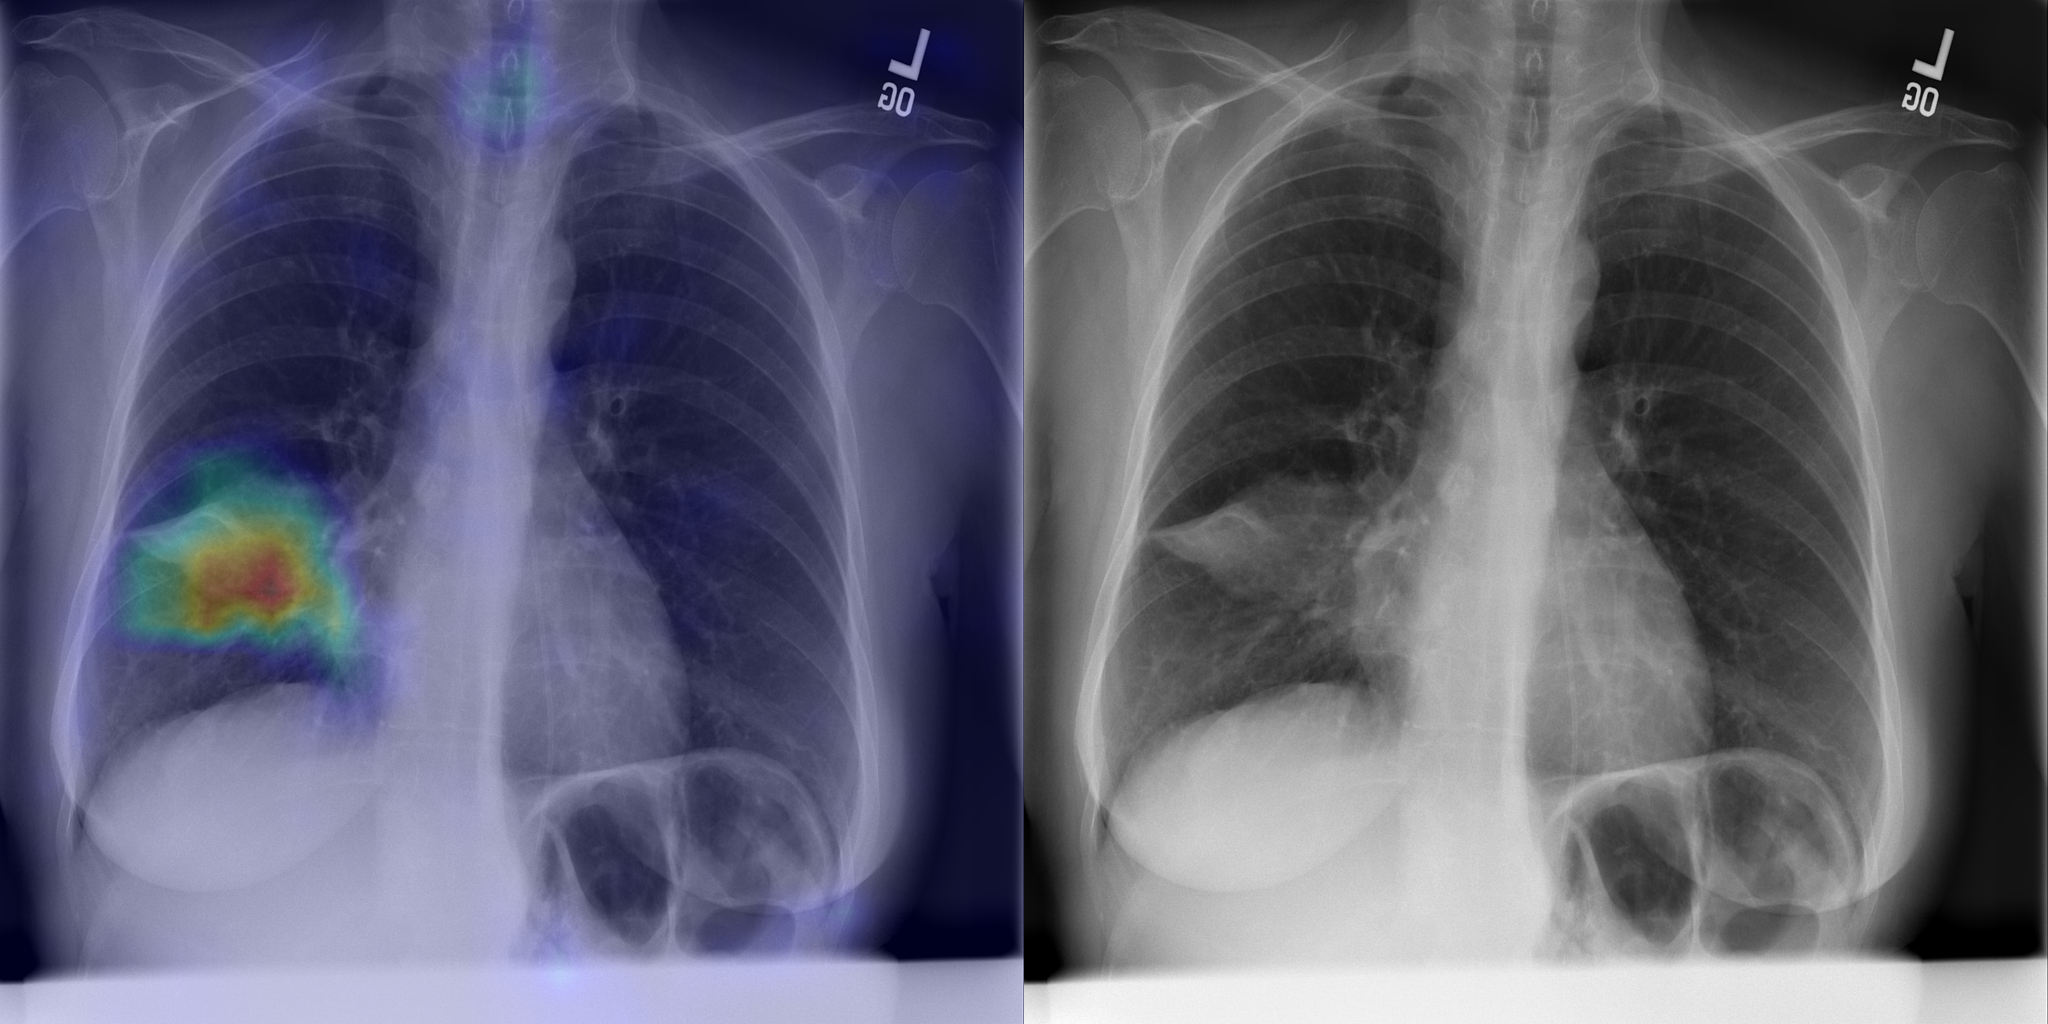
\includegraphics[width=1.0\textwidth]{Chapters/5. Conclusiones/img/Consolidation/1_1_00000618_011.png}
    \end{subfigure}
    \begin{subfigure}{0.4\textwidth}
        \centering
        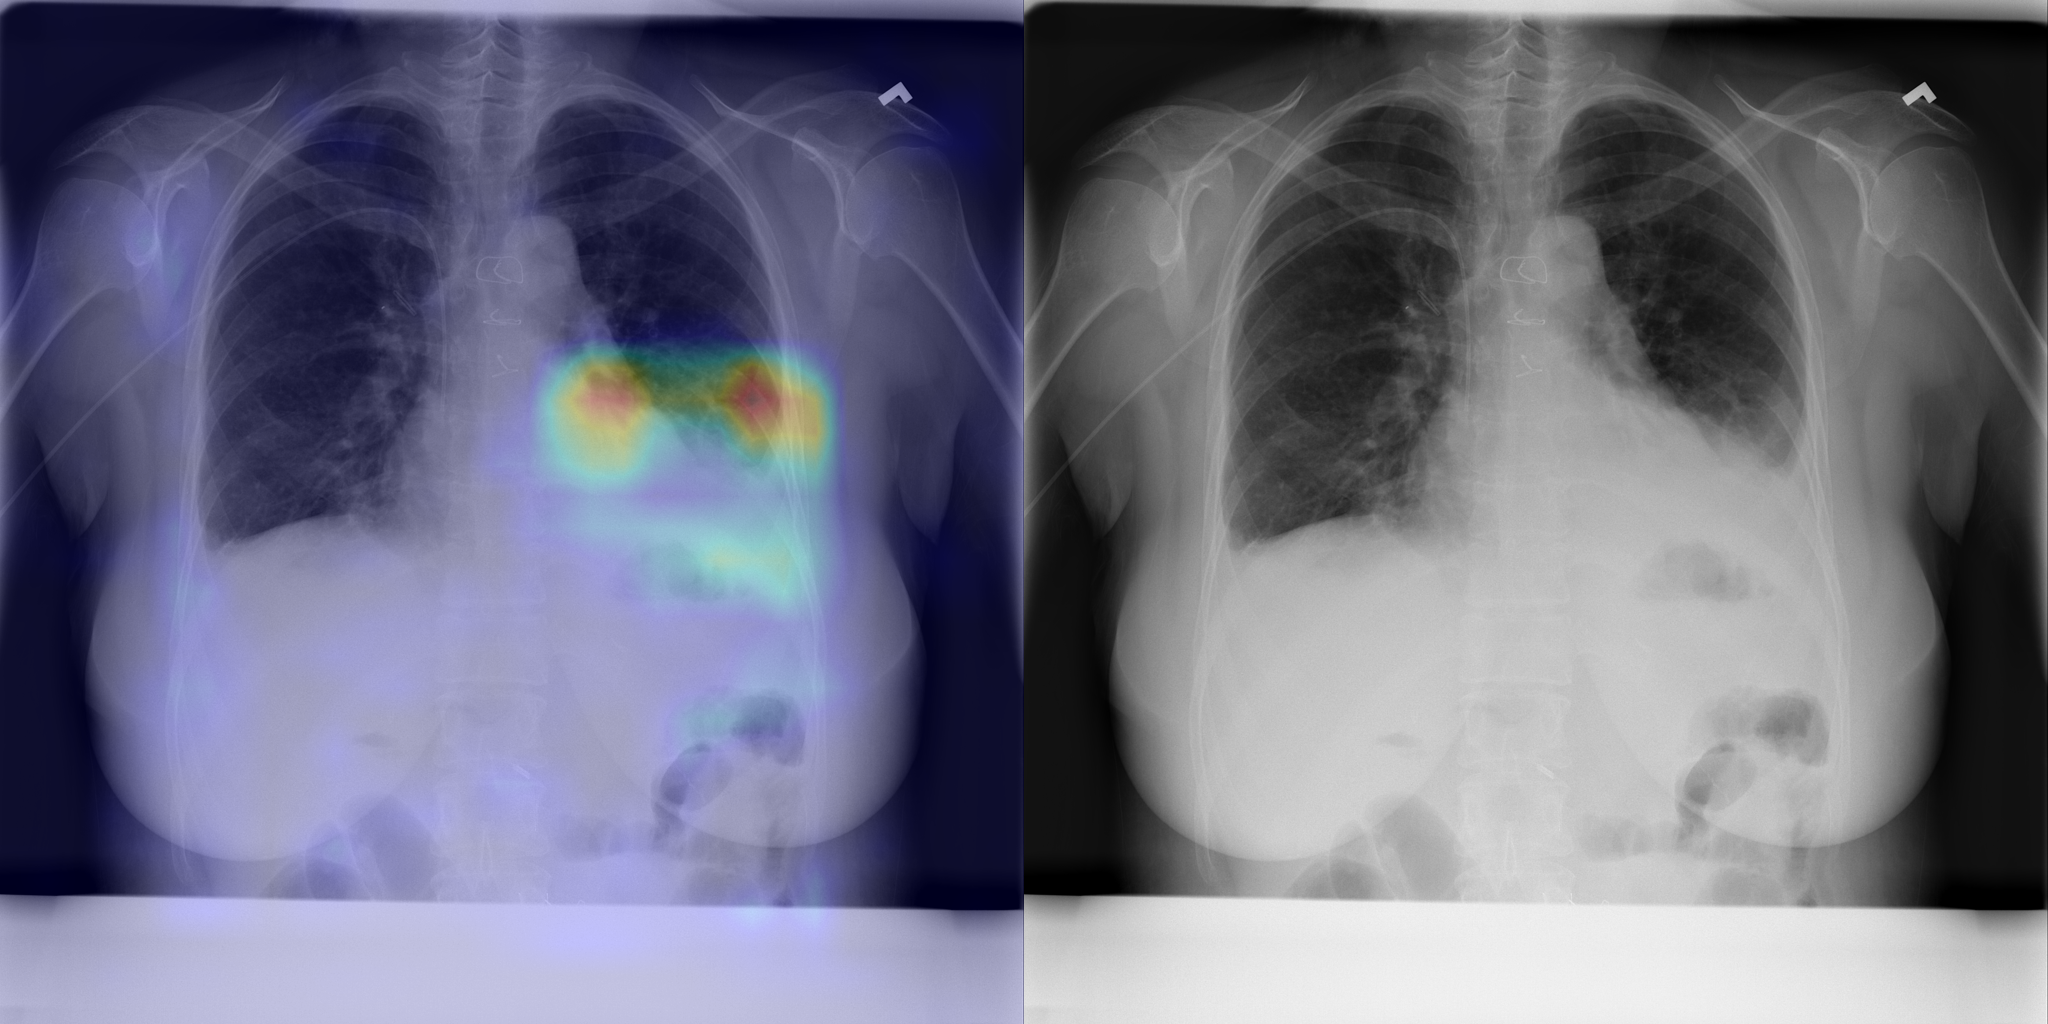
\includegraphics[width=1.0\textwidth]{Chapters/5. Conclusiones/img/Consolidation/1_1_00000808_002.png}
    \end{subfigure}
    \begin{subfigure}{0.4\textwidth}
        \centering
        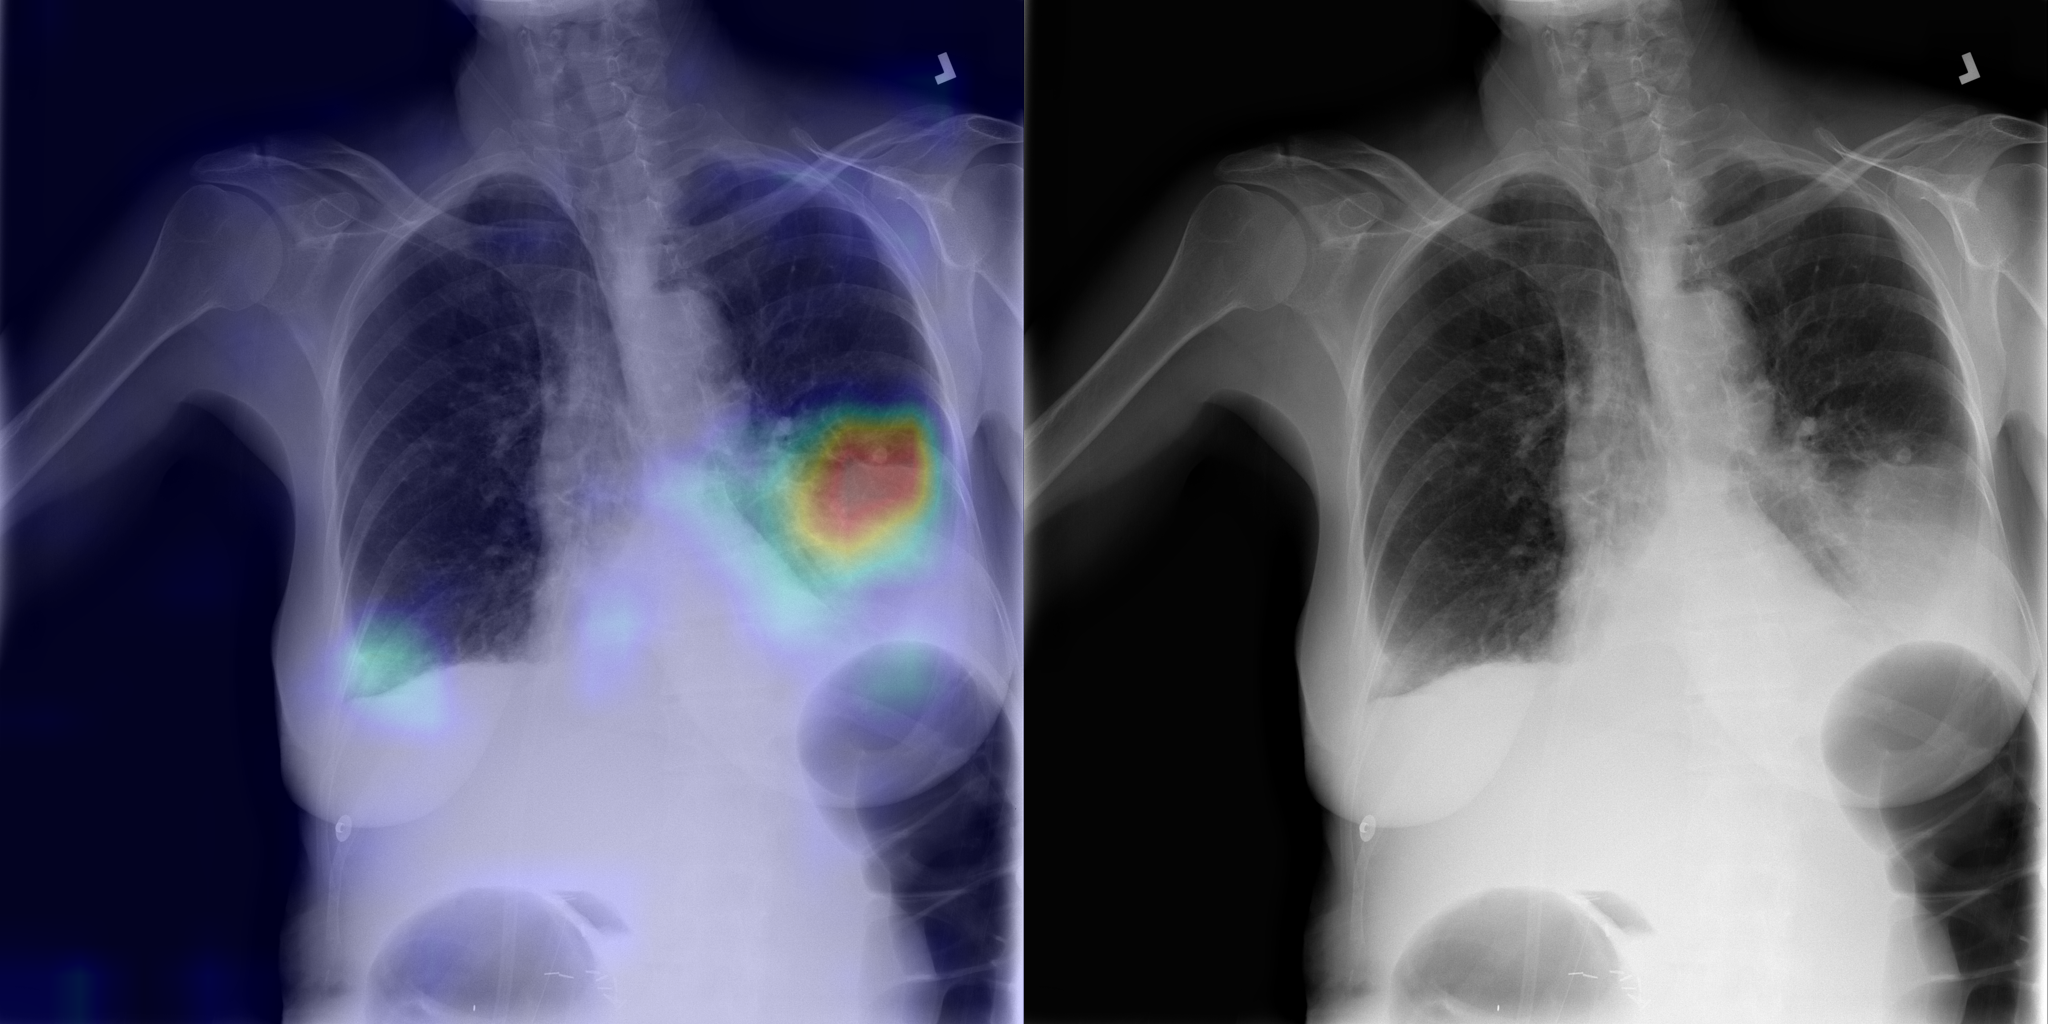
\includegraphics[width=1.0\textwidth]{Chapters/5. Conclusiones/img/Consolidation/1_1_00000882_003.png}
    \end{subfigure}
    \begin{subfigure}{0.4\textwidth}
        \centering
        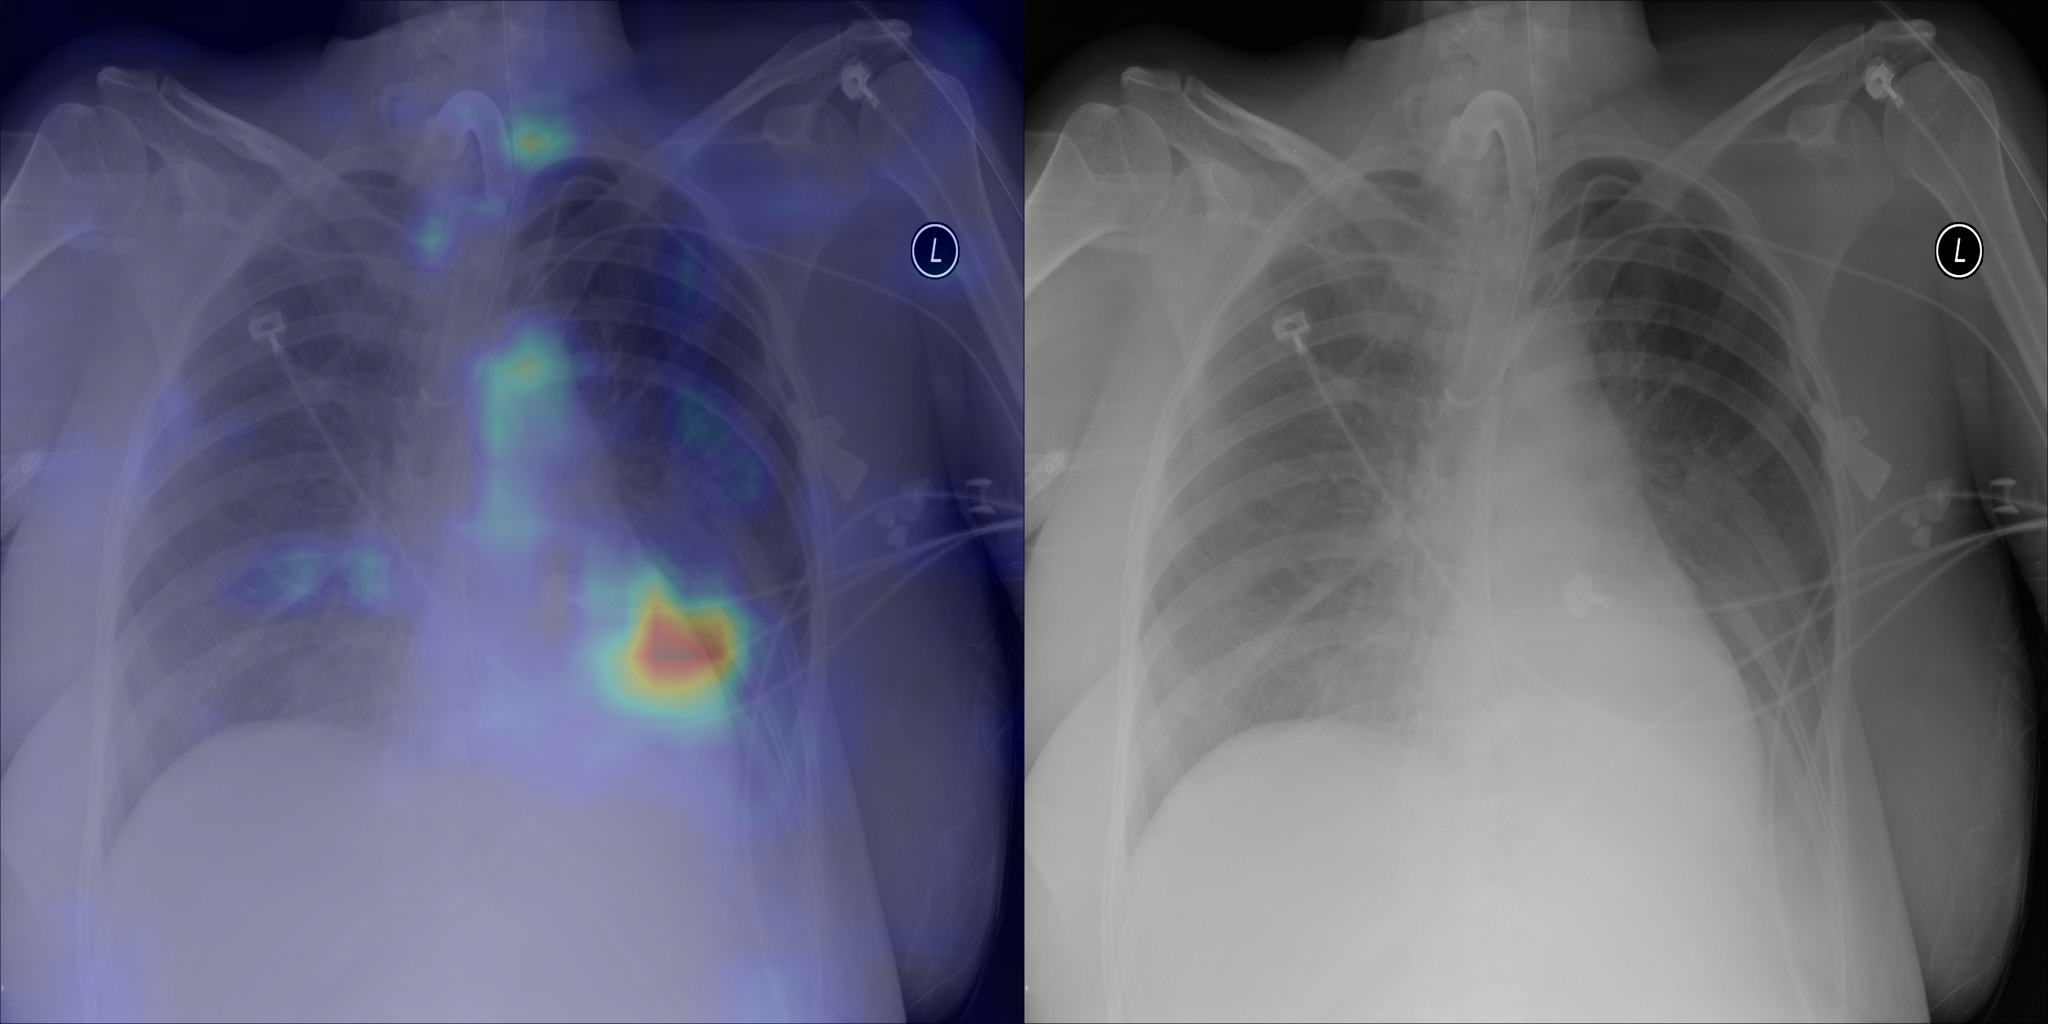
\includegraphics[width=1.0\textwidth]{Chapters/5. Conclusiones/img/Consolidation/1_1_00018187_052.png}
    \end{subfigure}

    \caption{Consolidación pulmunar. Radiografías detectadas con la patología de consolidación pulmunar por los
                    radiólogos. A la izquierda de cada imagen el GradCam correspondiente a la detección
                    de la patología como positivo por el modelo CNN.}
\end{figure}

\begin{figure}[b]
    \centering
    \begin{subfigure}{0.4\textwidth}
        \centering
        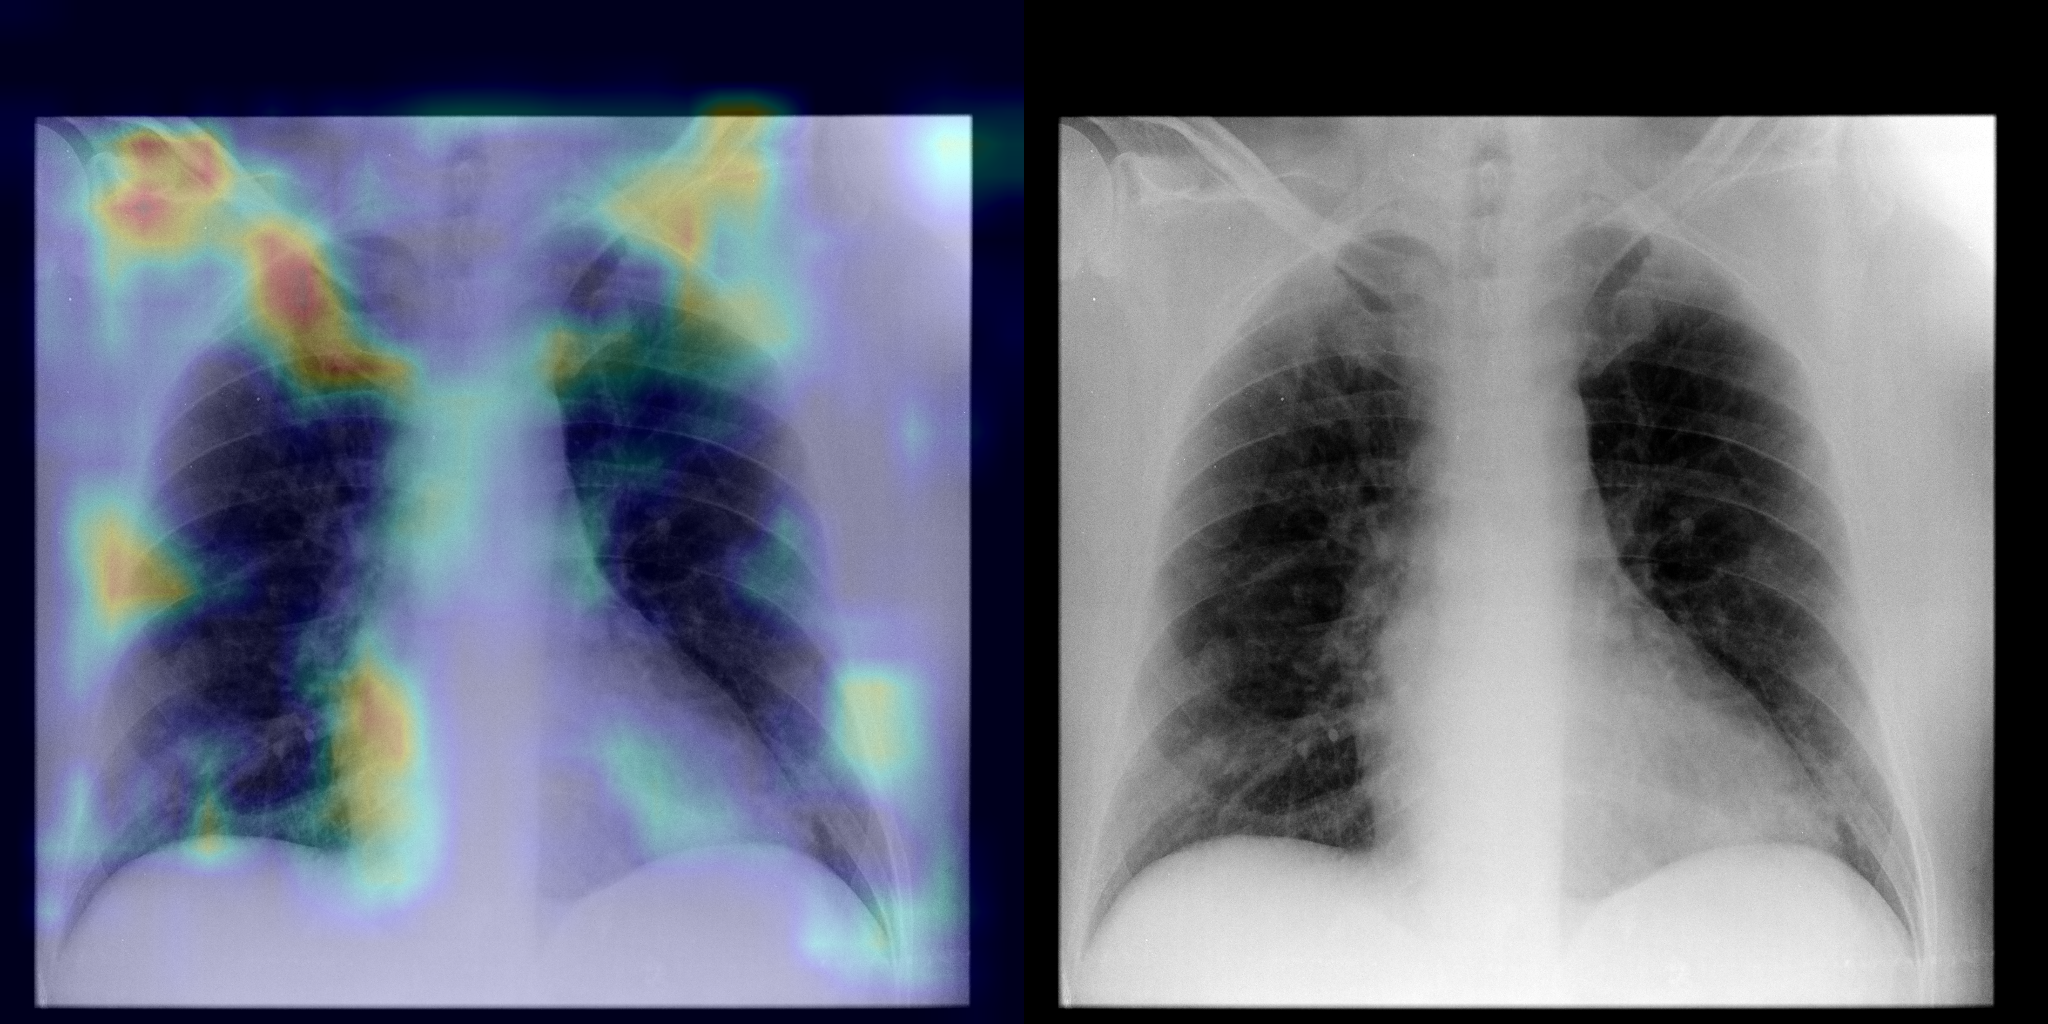
\includegraphics[width=1.0\textwidth]{Chapters/5. Conclusiones/img/COVID-19/1_1_0c9b15035c41_3ea703bd1e0b.png}
    \end{subfigure}
    \begin{subfigure}{0.4\textwidth}
        \centering
        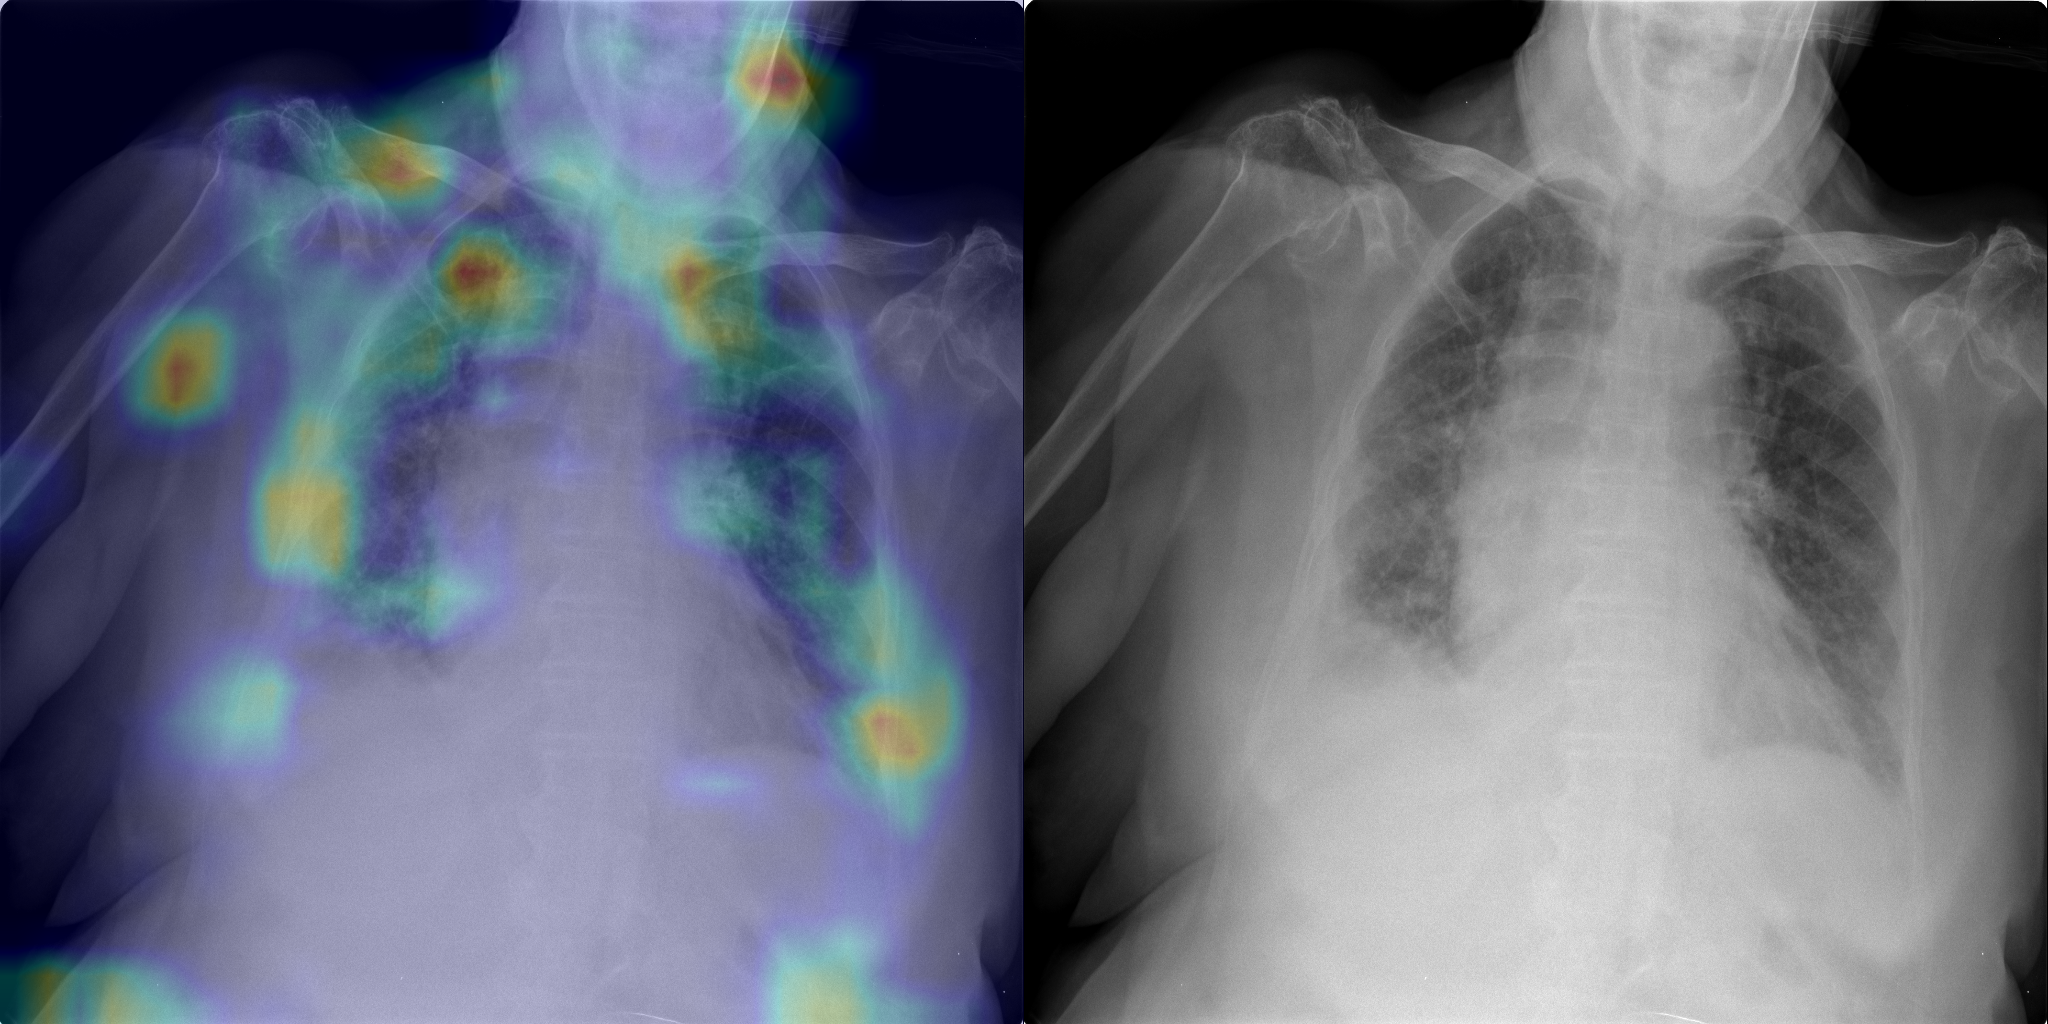
\includegraphics[width=1.0\textwidth]{Chapters/5. Conclusiones/img/COVID-19/1_1_0d5082a9a044_d417f8e64511.png}
    \end{subfigure}
    \begin{subfigure}{0.4\textwidth}
        \centering
        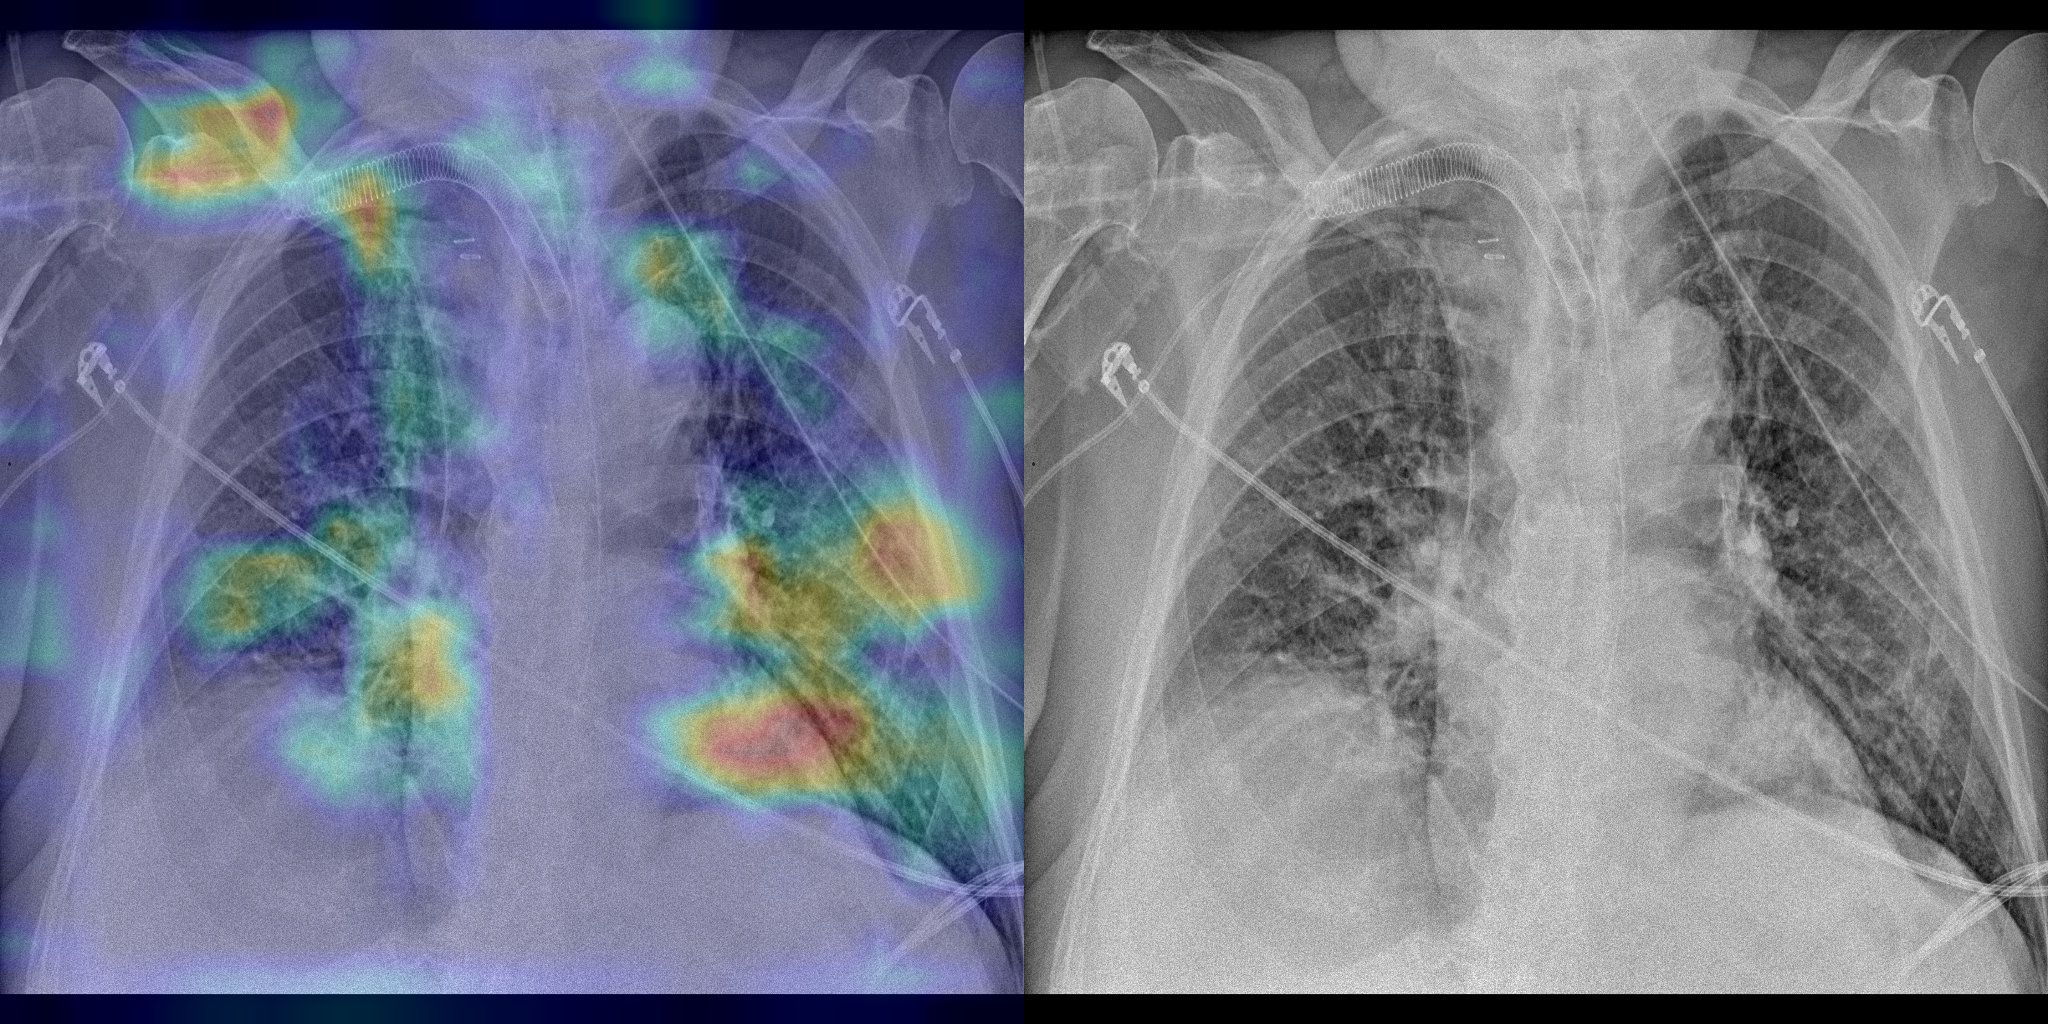
\includegraphics[width=1.0\textwidth]{Chapters/5. Conclusiones/img/COVID-19/1_1_1b5ca94ac38b_68fcf433c6fe.png}
    \end{subfigure}
    \begin{subfigure}{0.4\textwidth}
        \centering
        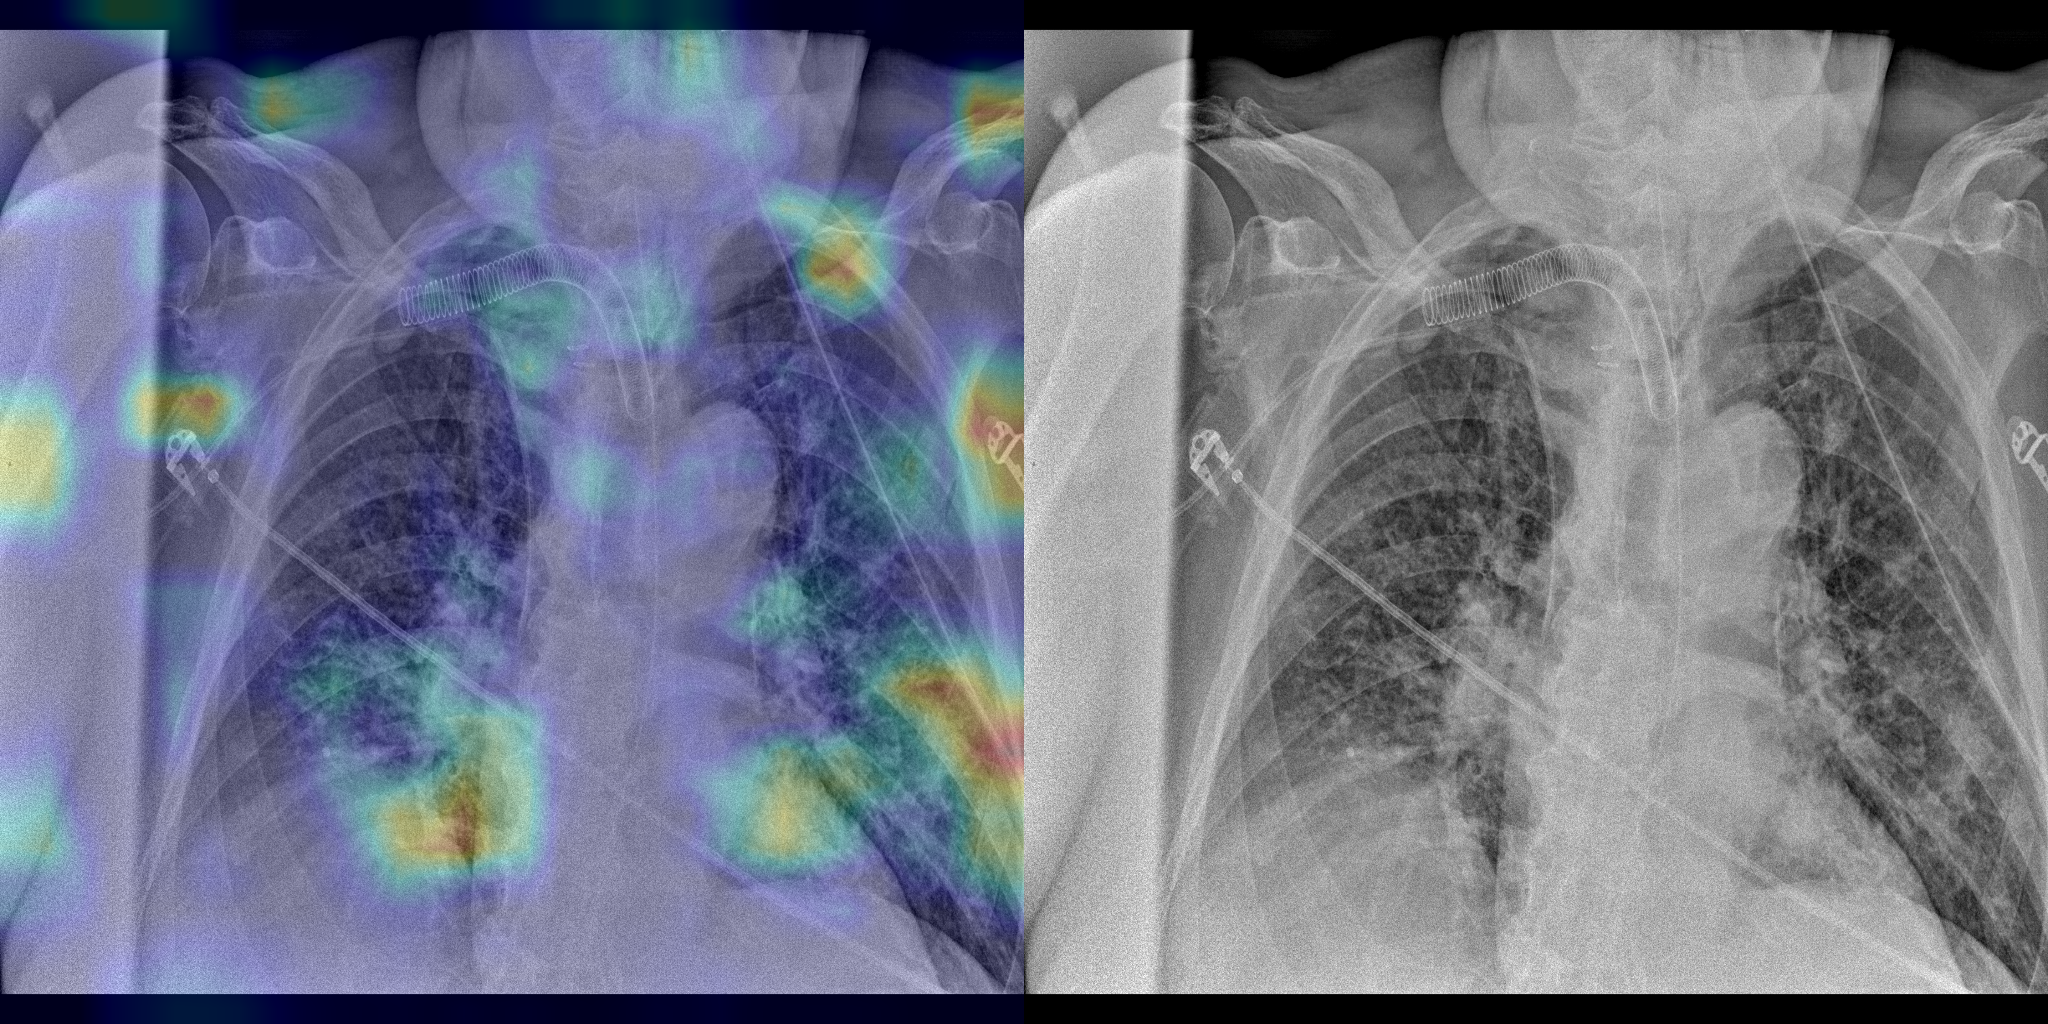
\includegraphics[width=1.0\textwidth]{Chapters/5. Conclusiones/img/COVID-19/1_1_1b5ca94ac38b_0919a3b8af01.png}
    \end{subfigure}
    \begin{subfigure}{0.4\textwidth}
        \centering
        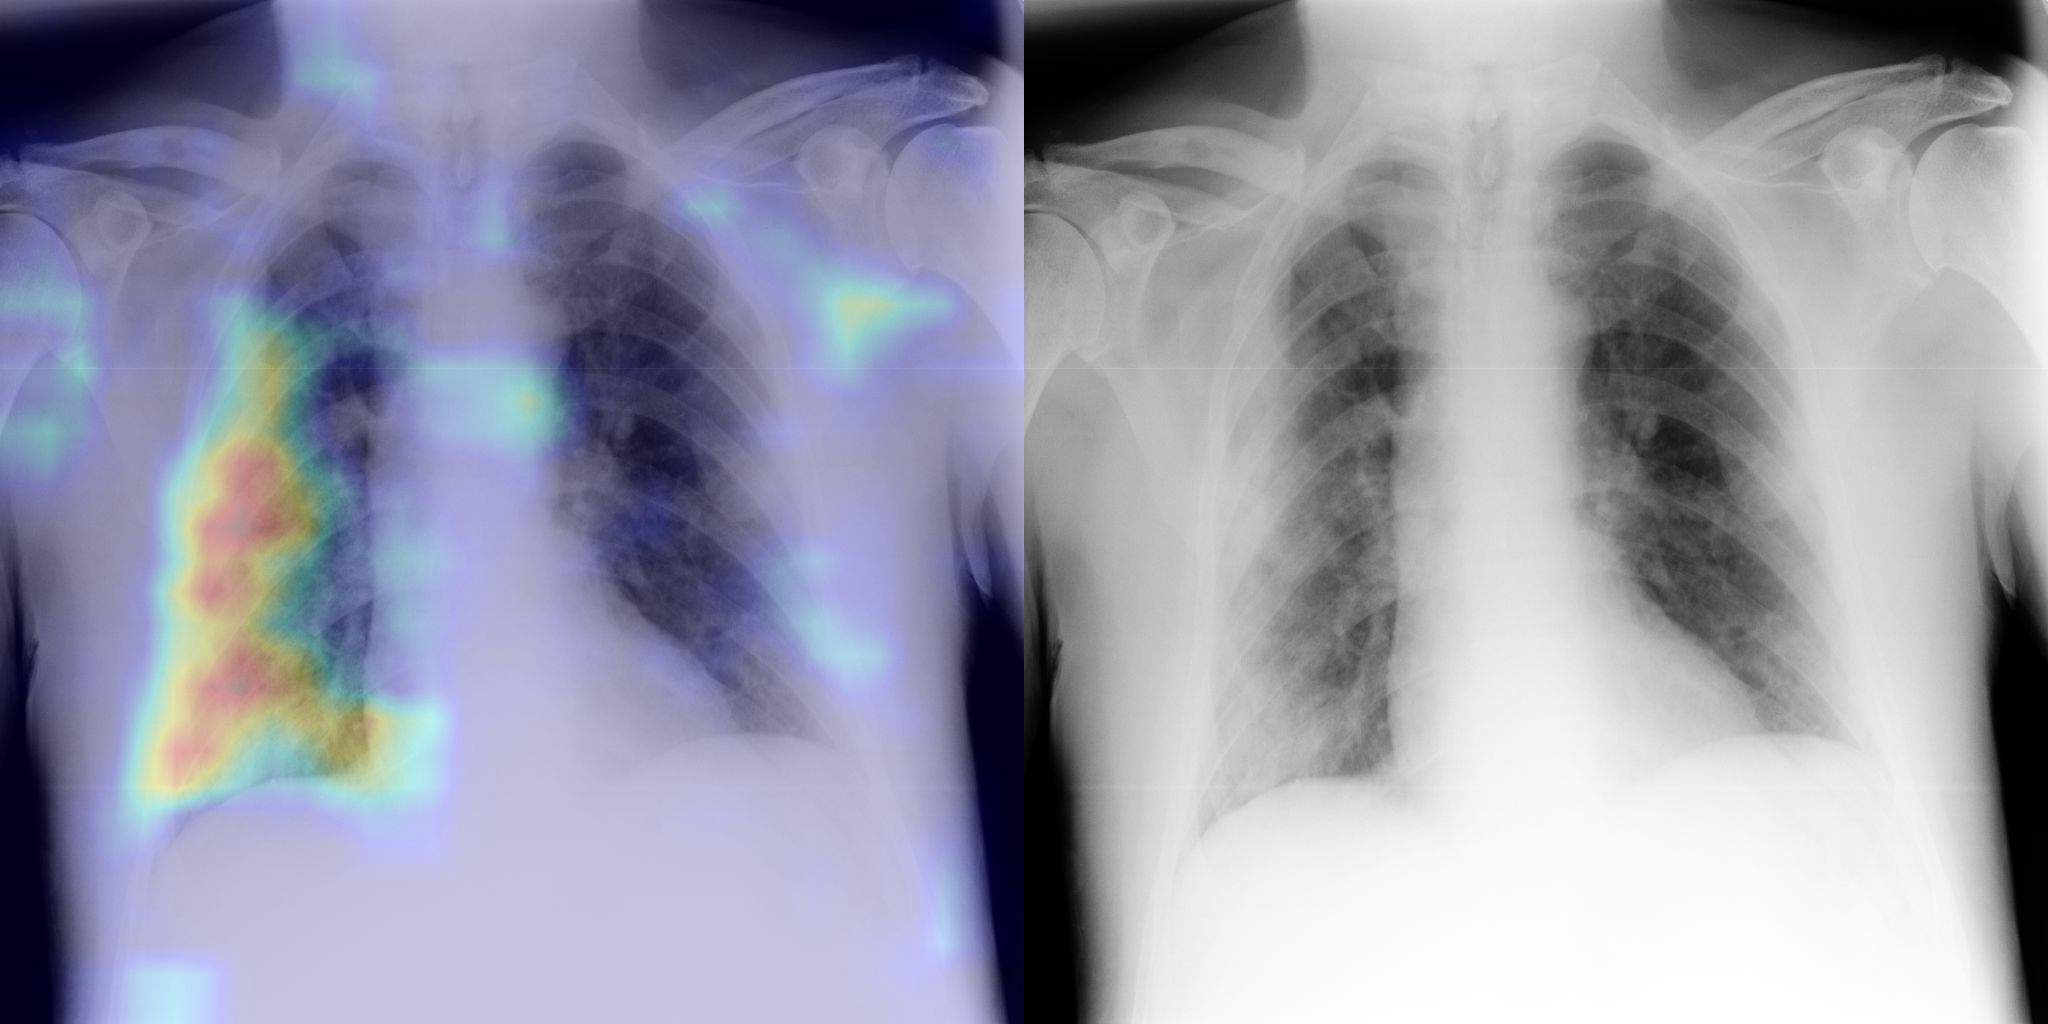
\includegraphics[width=1.0\textwidth]{Chapters/5. Conclusiones/img/COVID-19/1_1_1e3f6f8e494c_efe83e860c17.png}
    \end{subfigure}
    \begin{subfigure}{0.4\textwidth}
        \centering
        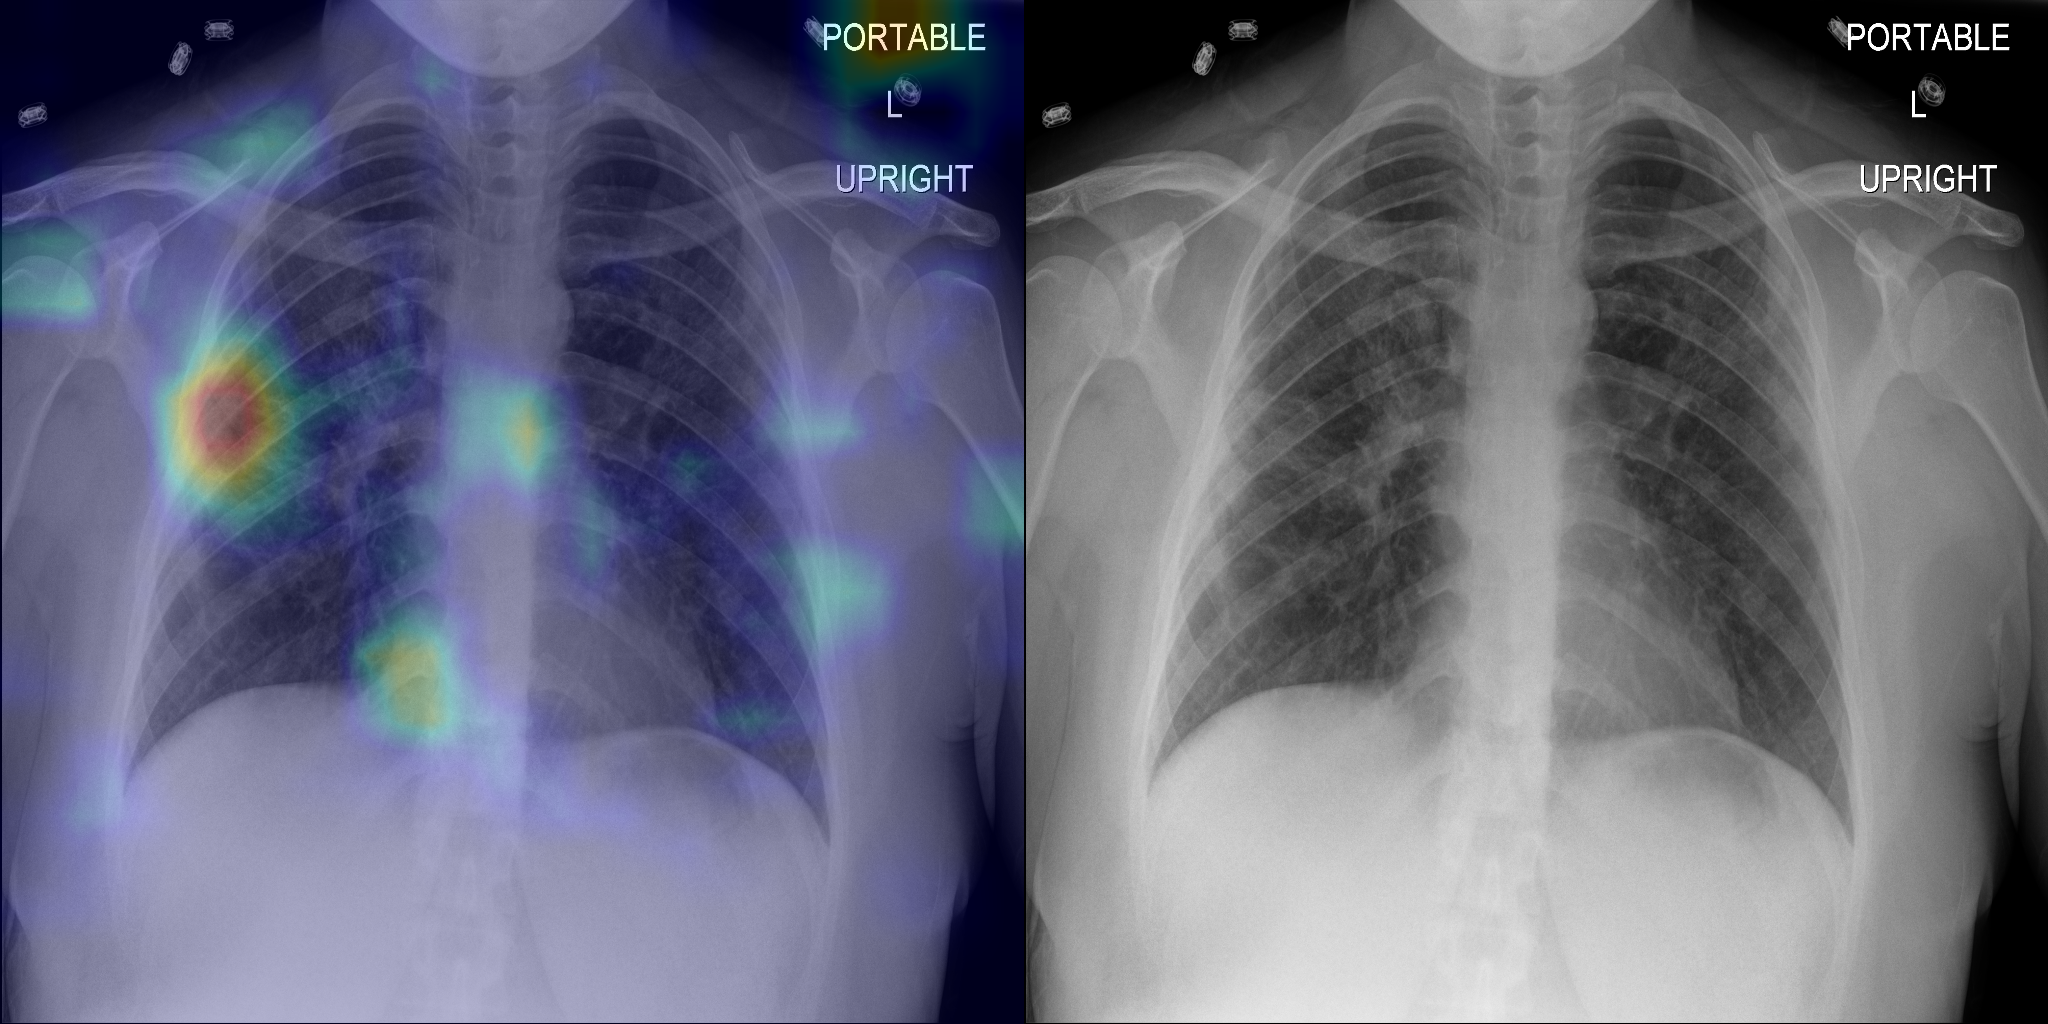
\includegraphics[width=1.0\textwidth]{Chapters/5. Conclusiones/img/COVID-19/1_1_4bb14a344446_0d3910133fbe.png}
    \end{subfigure}
    \begin{subfigure}{0.4\textwidth}
        \centering
        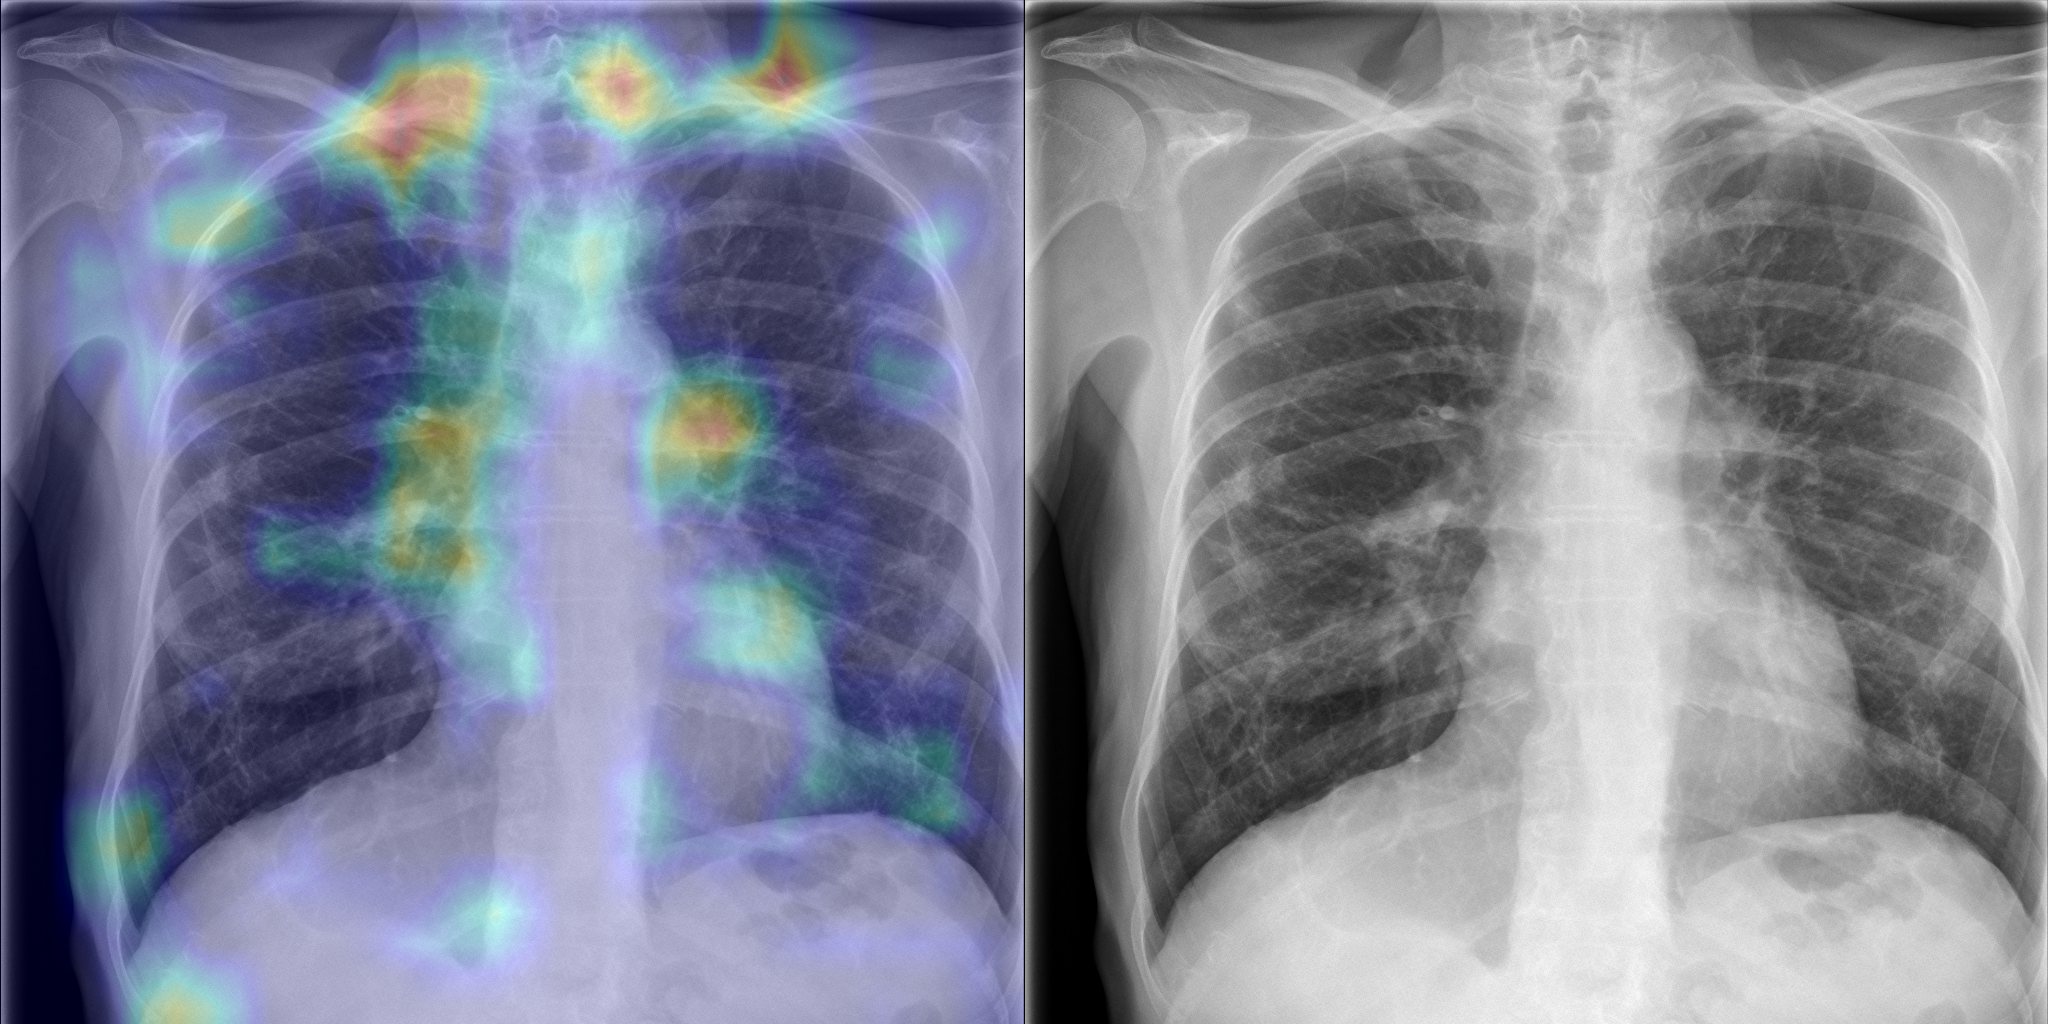
\includegraphics[width=1.0\textwidth]{Chapters/5. Conclusiones/img/COVID-19/1_1_4be426760e00_16d85c7f7837.png}
    \end{subfigure}
    \begin{subfigure}{0.4\textwidth}
        \centering
        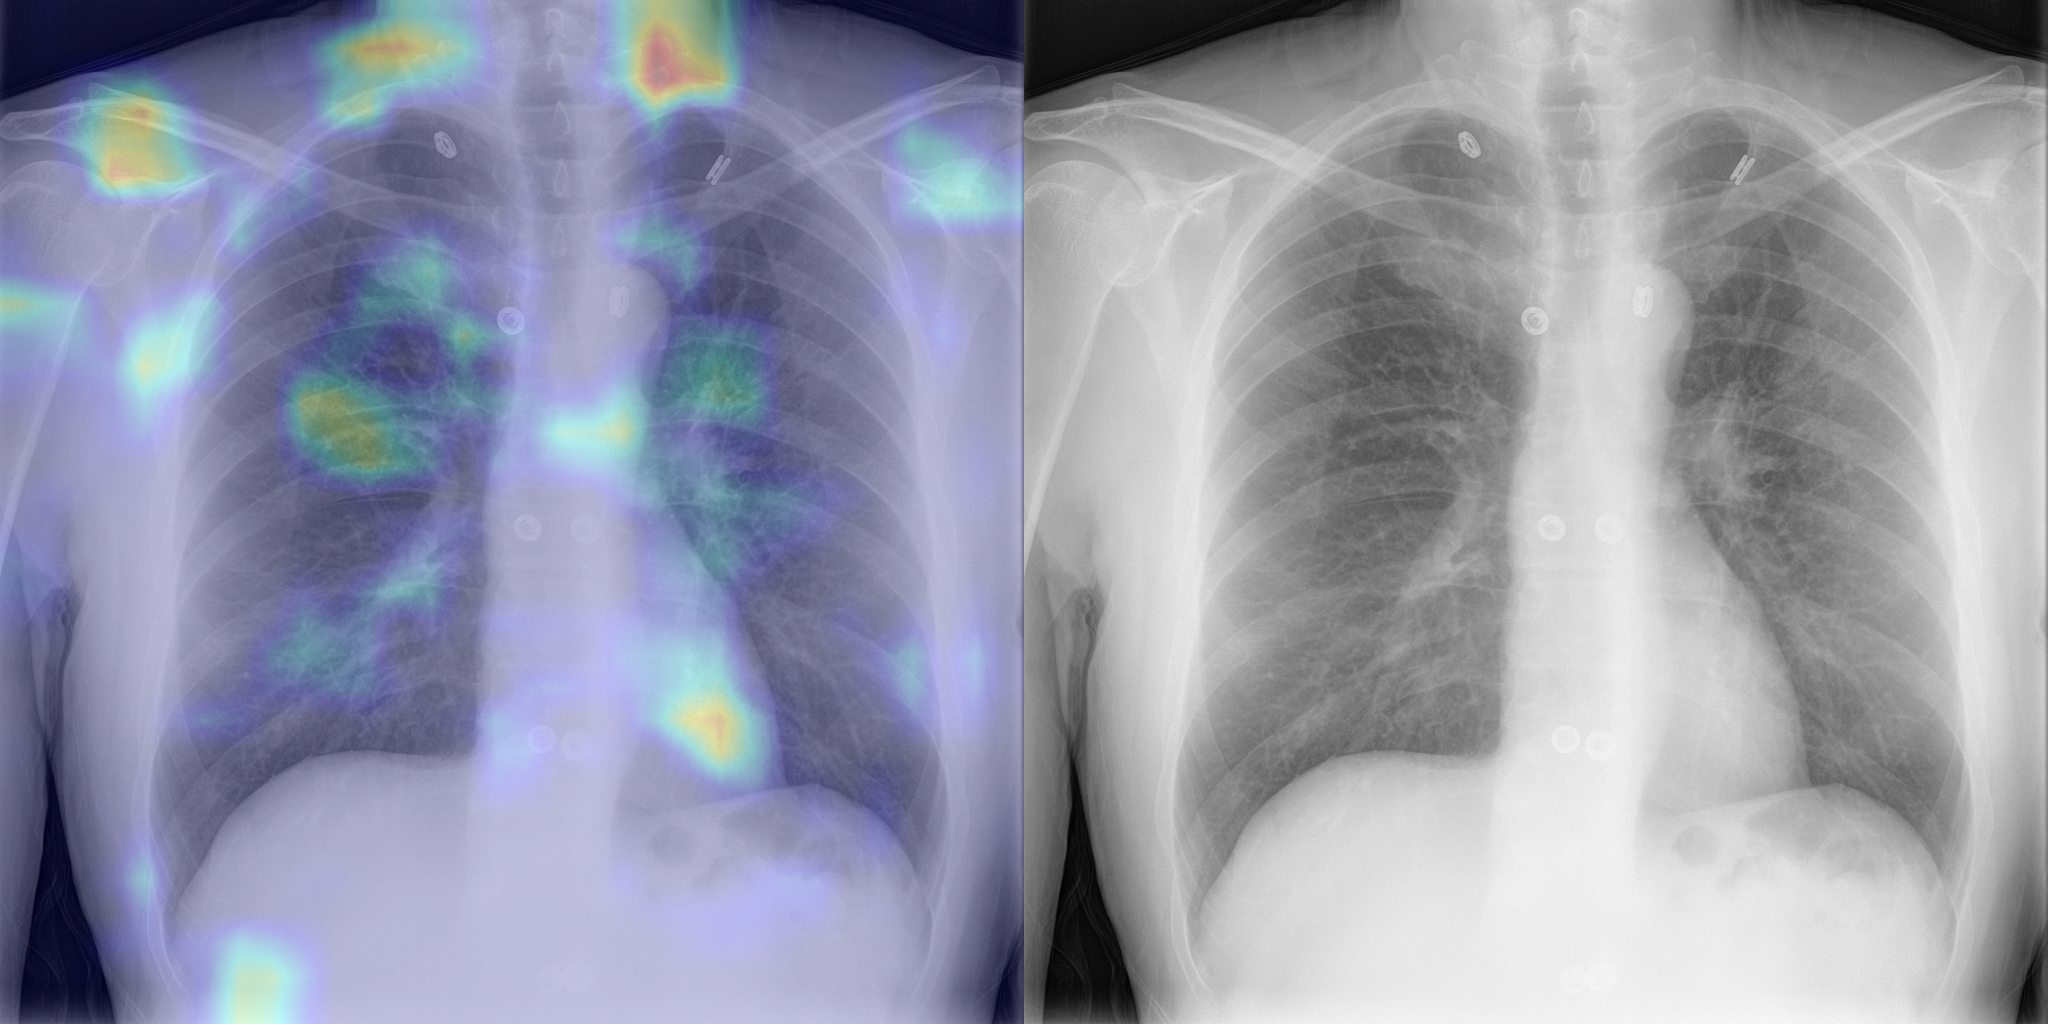
\includegraphics[width=1.0\textwidth]{Chapters/5. Conclusiones/img/COVID-19/1_1_7b6c49da06db_b6b631939d4f.png}
    \end{subfigure}
    \begin{subfigure}{0.4\textwidth}
        \centering
        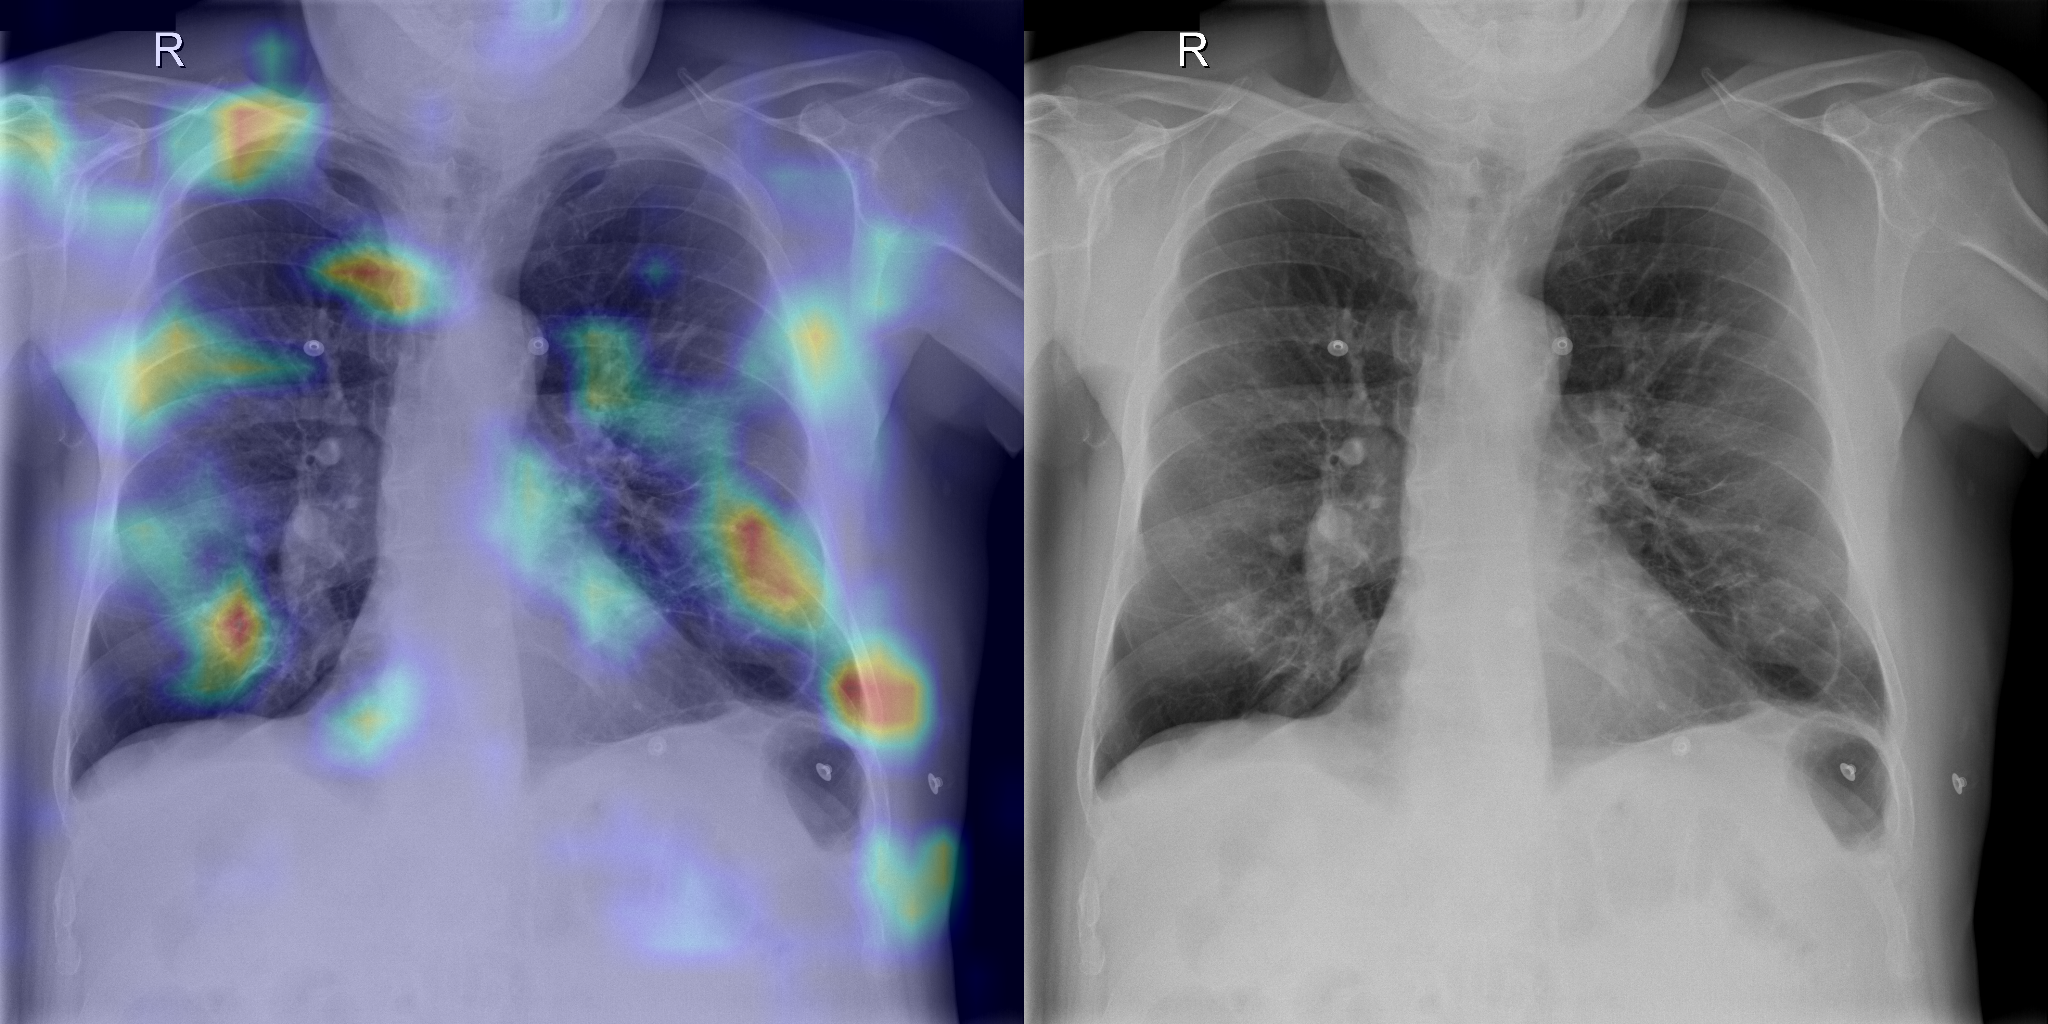
\includegraphics[width=1.0\textwidth]{Chapters/5. Conclusiones/img/COVID-19/1_1_cde0ab9526da_fa935d855d4e.png}
    \end{subfigure}
    \begin{subfigure}{0.4\textwidth}
        \centering
        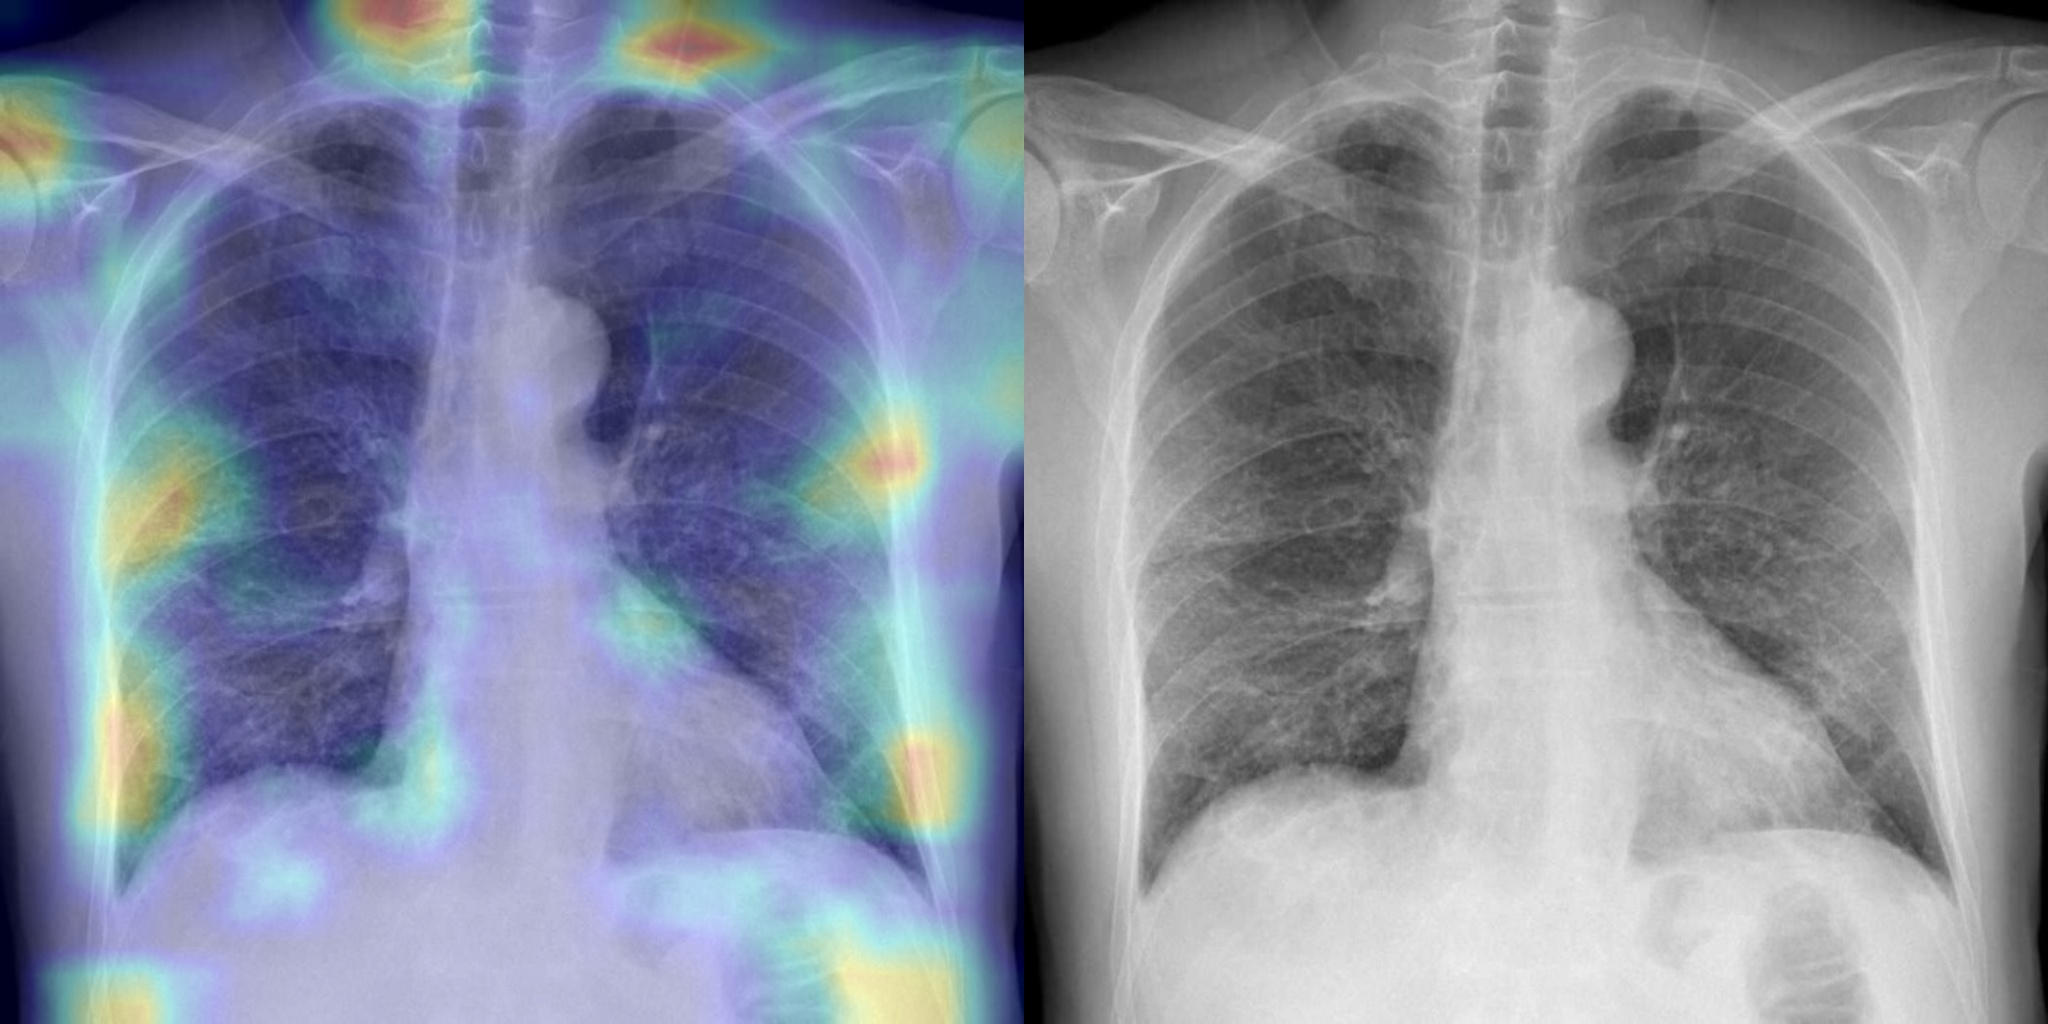
\includegraphics[width=1.0\textwidth]{Chapters/5. Conclusiones/img/COVID-19/1_1_covid-19-pneumonia-20-pa-on-admission.jpg}
    \end{subfigure}

    \caption{Covid-19. Radiografías detectadas con la patología de Covid-19 por los
                    radiólogos. A la izquierda de cada imagen el GradCam correspondiente a la detección
                    de la patología como positivo por el modelo CNN.}
\end{figure}

\begin{figure}[b]
    \centering
    \begin{subfigure}{0.4\textwidth}
        \centering
        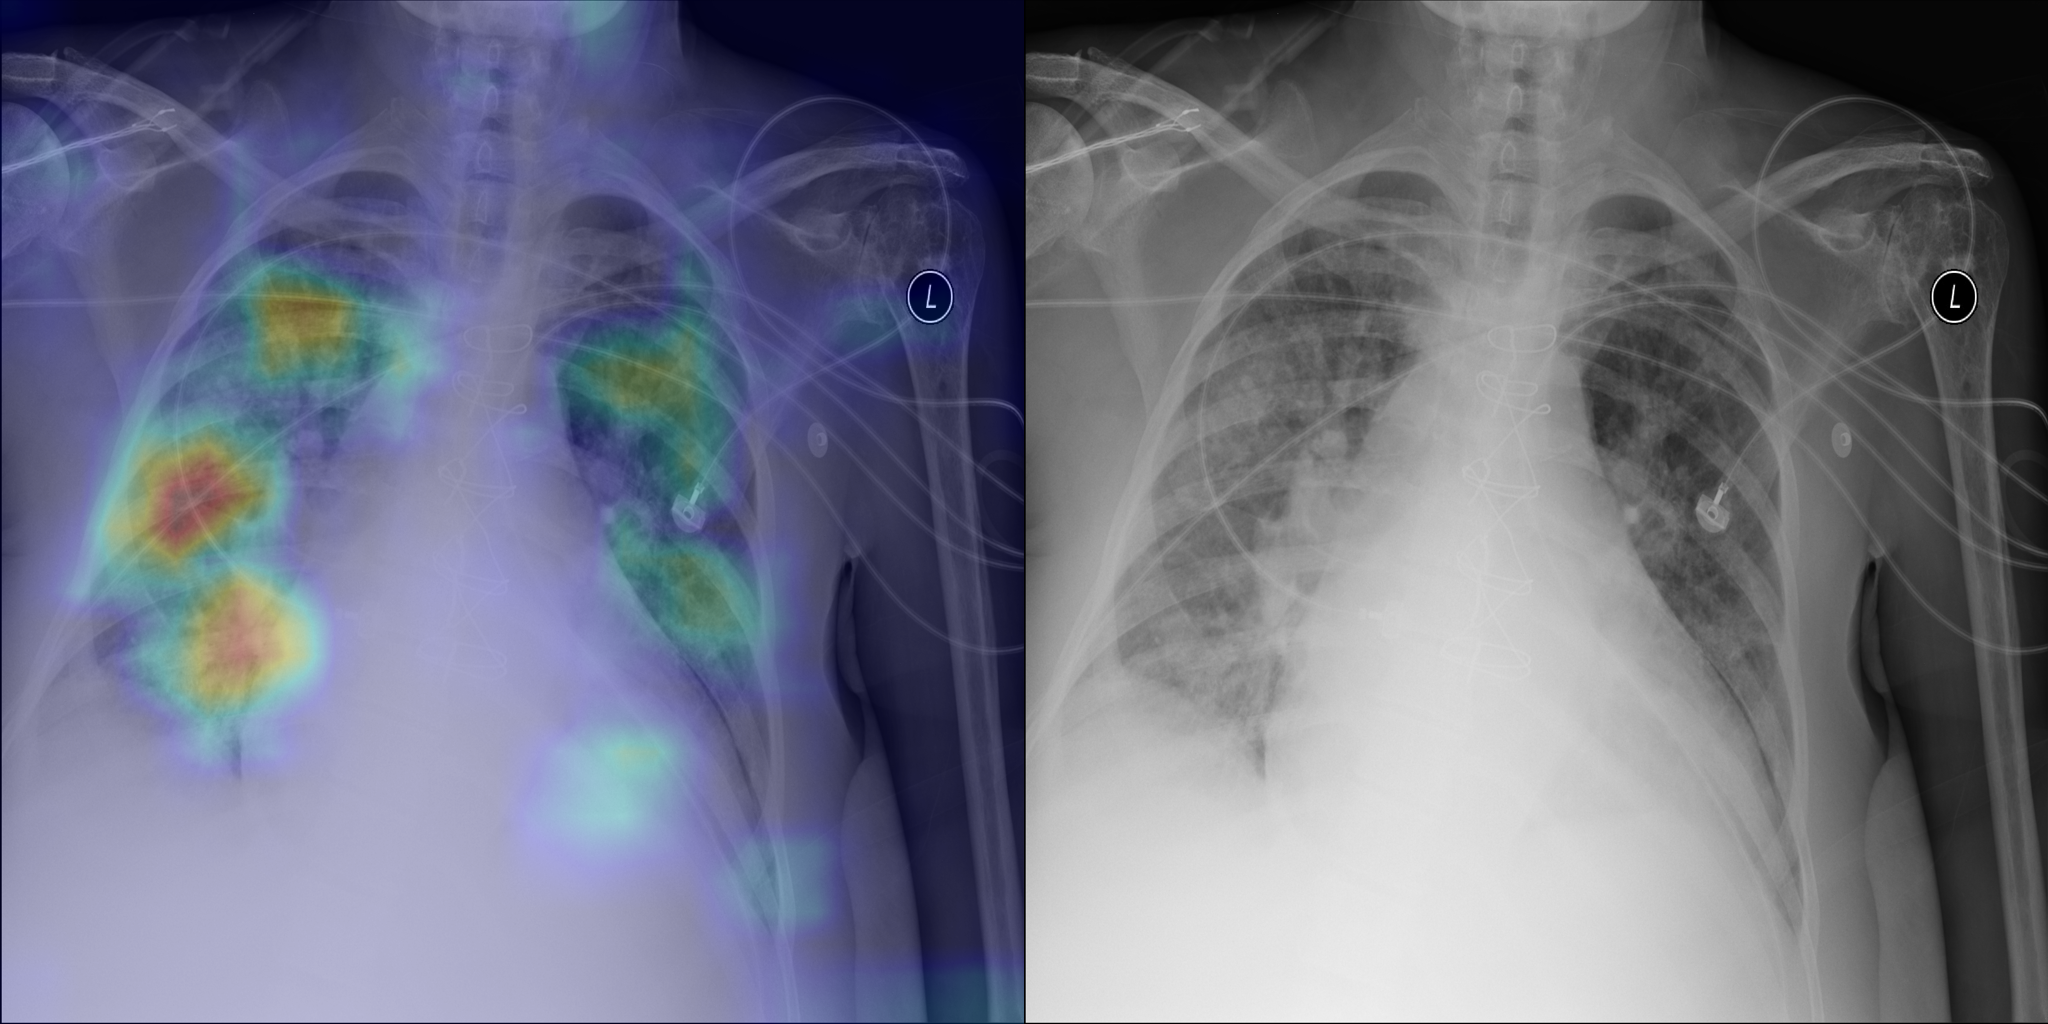
\includegraphics[width=1.0\textwidth]{Chapters/5. Conclusiones/img/Edema/1_1_00001373_031.png}
    \end{subfigure}
    \begin{subfigure}{0.4\textwidth}
        \centering
        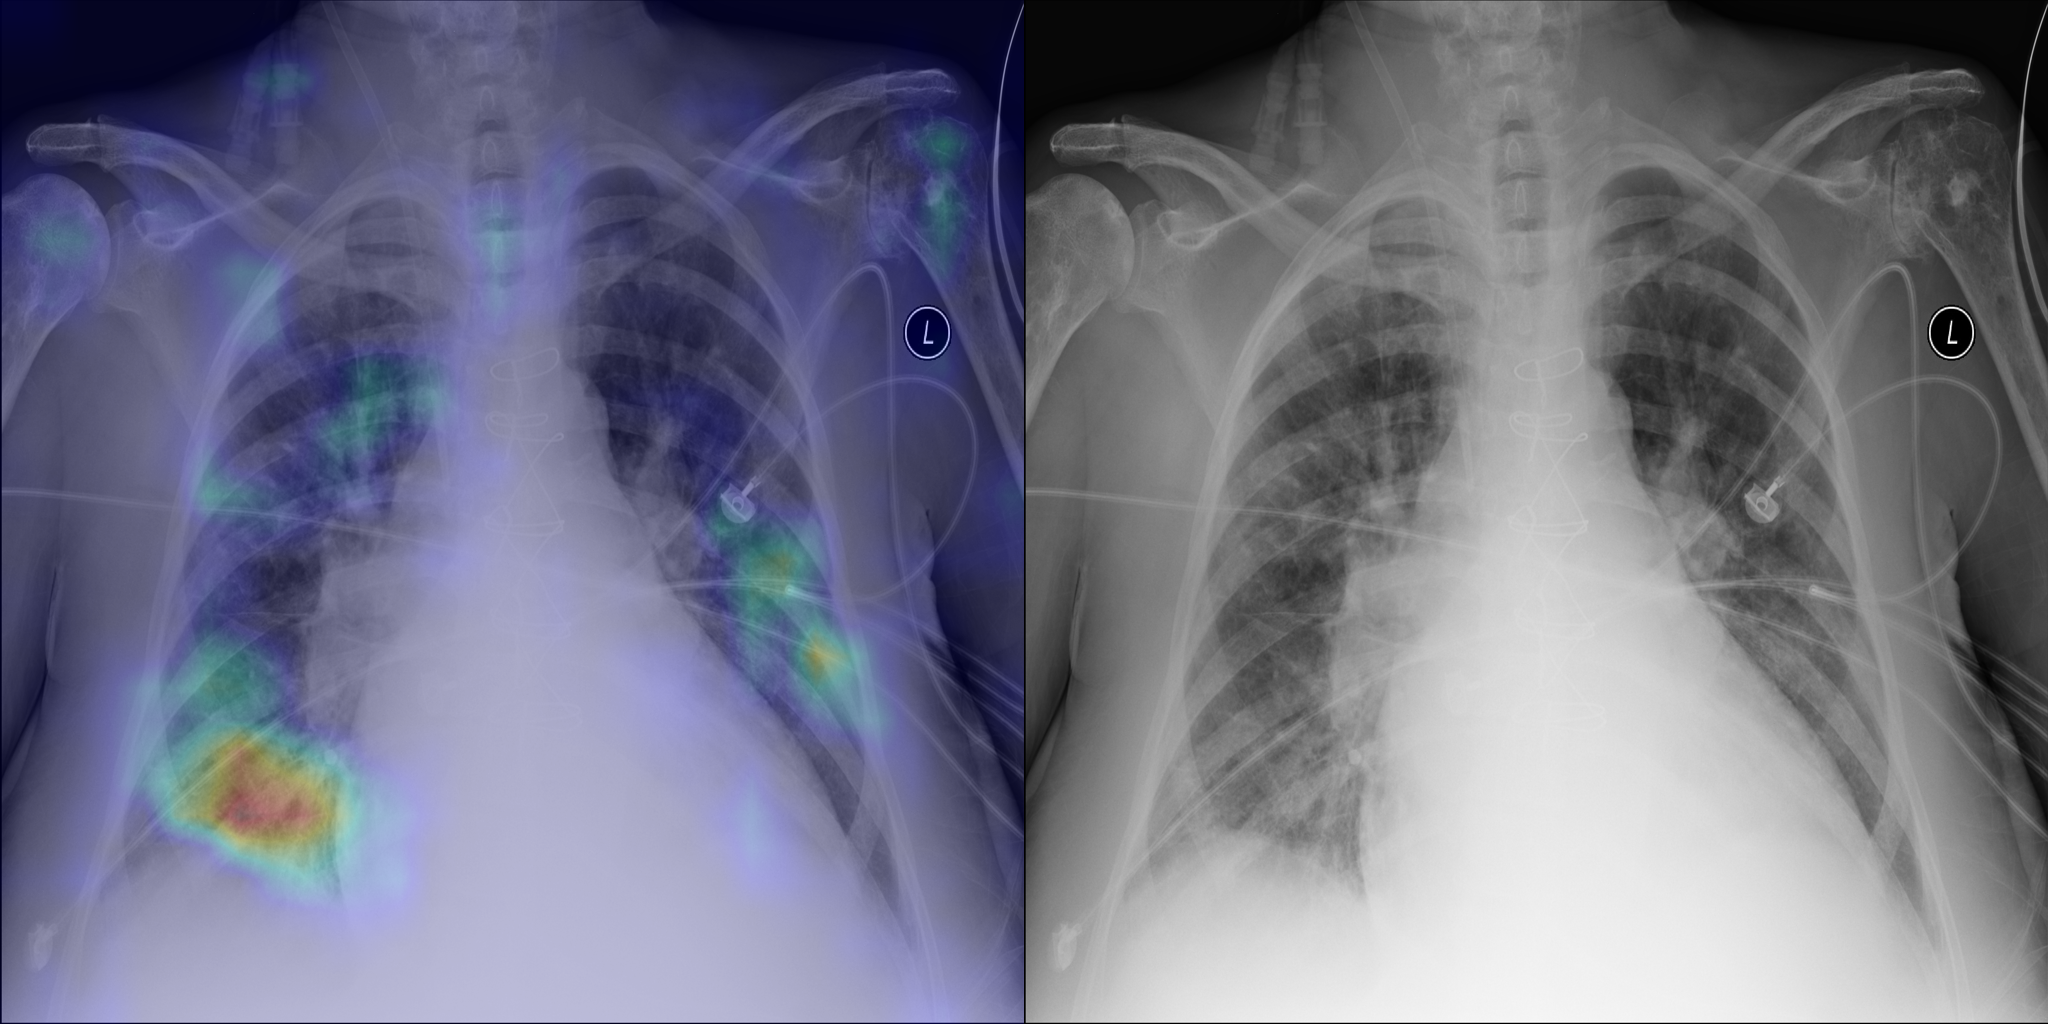
\includegraphics[width=1.0\textwidth]{Chapters/5. Conclusiones/img/Edema/1_1_00001373_032.png}
    \end{subfigure}
    \begin{subfigure}{0.4\textwidth}
        \centering
        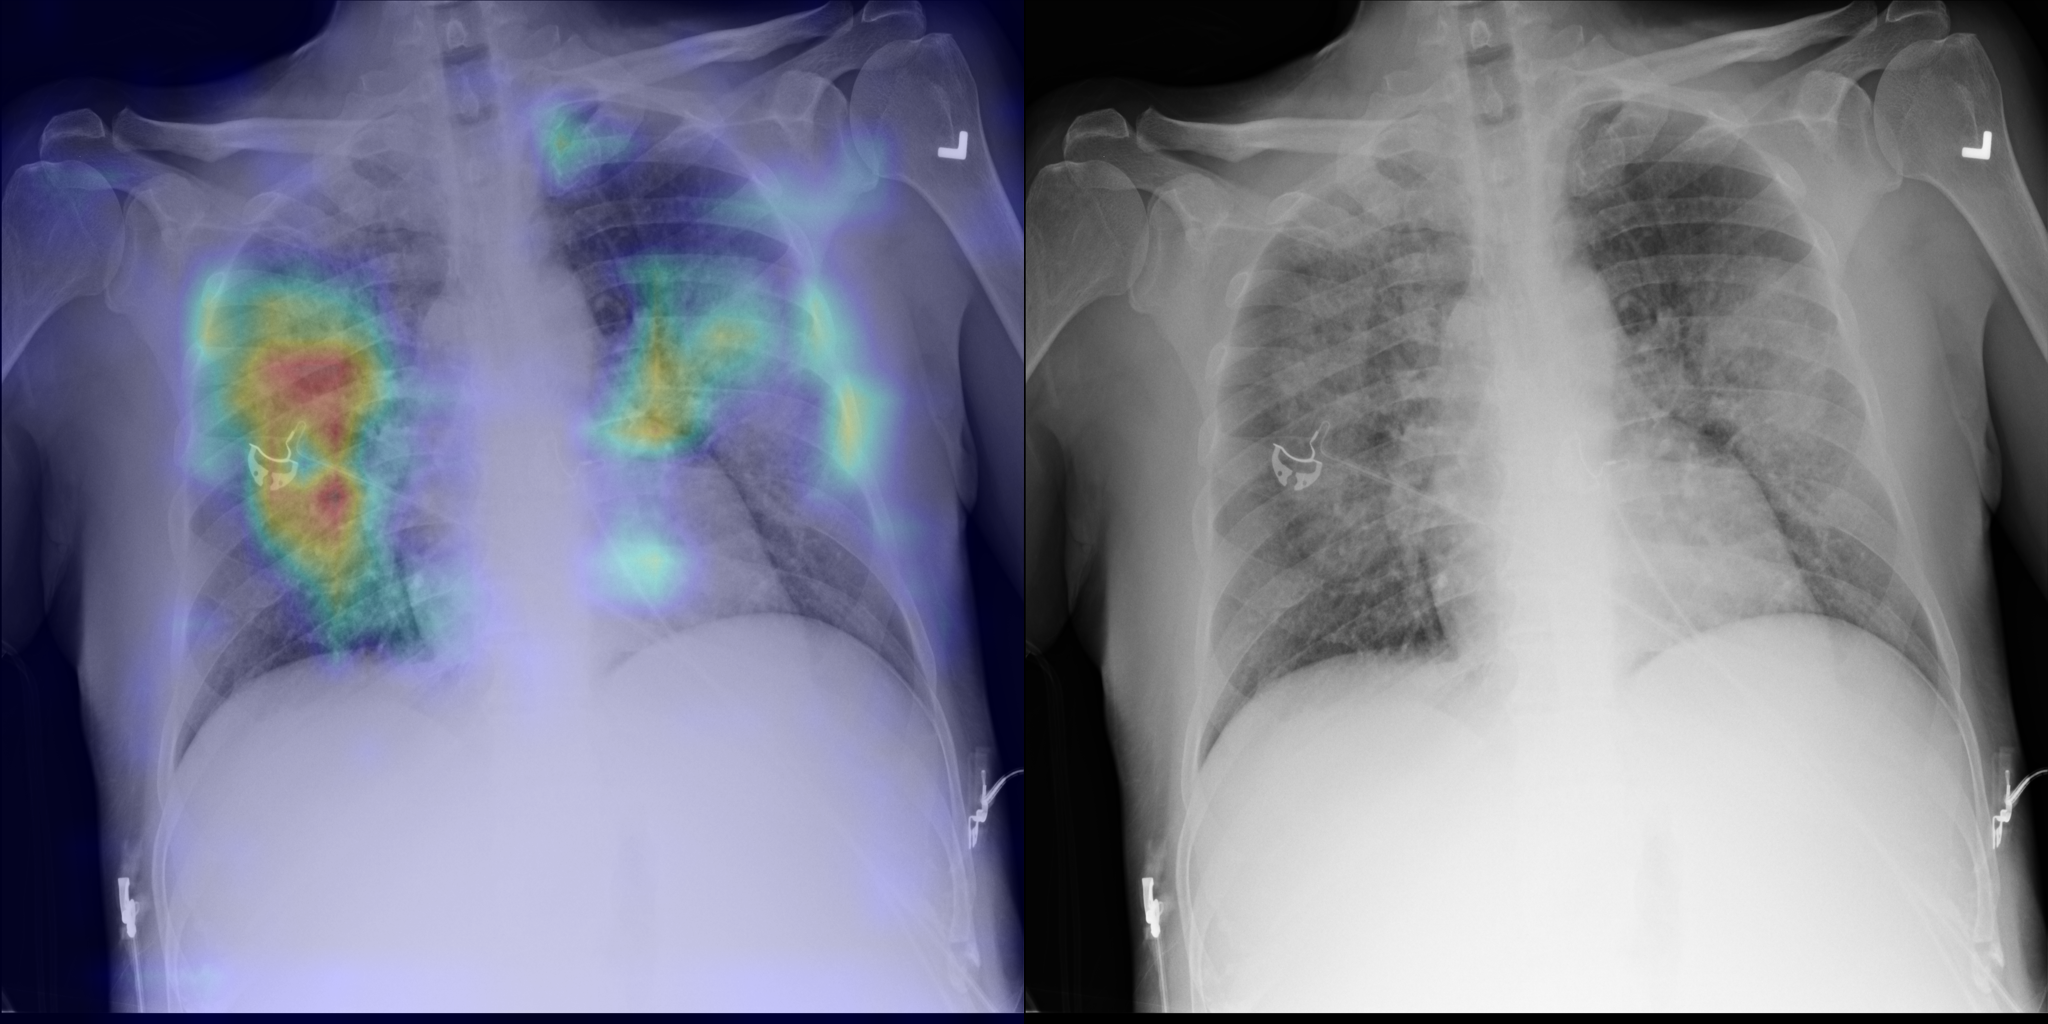
\includegraphics[width=1.0\textwidth]{Chapters/5. Conclusiones/img/Edema/1_1_00001787_000.png}
    \end{subfigure}
    \begin{subfigure}{0.4\textwidth}
        \centering
        \includegraphics[width=1.0\textwidth]{Chapters/5. Conclusiones/img/Edema/1_1_00003528_021.png}
    \end{subfigure}
    \begin{subfigure}{0.4\textwidth}
        \centering
        \includegraphics[width=1.0\textwidth]{Chapters/5. Conclusiones/img/Edema/1_1_00003803_009.png}
    \end{subfigure}
    \begin{subfigure}{0.4\textwidth}
        \centering
        \includegraphics[width=1.0\textwidth]{Chapters/5. Conclusiones/img/Edema/1_1_00004533_020.png}
    \end{subfigure}
    \begin{subfigure}{0.4\textwidth}
        \centering
        \includegraphics[width=1.0\textwidth]{Chapters/5. Conclusiones/img/Edema/1_1_00006304_002.png}
    \end{subfigure}
    \begin{subfigure}{0.4\textwidth}
        \centering
        \includegraphics[width=1.0\textwidth]{Chapters/5. Conclusiones/img/Edema/1_1_00006304_006.png}
    \end{subfigure}
    \begin{subfigure}{0.4\textwidth}
        \centering
        \includegraphics[width=1.0\textwidth]{Chapters/5. Conclusiones/img/Edema/1_1_00010535_002.png}
    \end{subfigure}
    \begin{subfigure}{0.4\textwidth}
        \centering
        \includegraphics[width=1.0\textwidth]{Chapters/5. Conclusiones/img/Edema/1_1_00011583_006.png}
    \end{subfigure}

    \caption{Edema. Radiografías detectadas con la patología de edema pulmonar por los
                    radiólogos. A la izquierda de cada imagen el GradCam correspondiente a la detección
                    de la patología como positivo por el modelo CNN.}
\end{figure}

\begin{figure}[b]
    \centering
    \begin{subfigure}{0.4\textwidth}
        \centering
        \includegraphics[width=1.0\textwidth]{Chapters/5. Conclusiones/img/Effusion/1_1_00000092_001.png}
    \end{subfigure}
    \begin{subfigure}{0.4\textwidth}
        \centering
        \includegraphics[width=1.0\textwidth]{Chapters/5. Conclusiones/img/Effusion/1_1_00000147_002.png}
    \end{subfigure}
    \begin{subfigure}{0.4\textwidth}
        \centering
        \includegraphics[width=1.0\textwidth]{Chapters/5. Conclusiones/img/Effusion/1_1_00000181_005.png}
    \end{subfigure}
    \begin{subfigure}{0.4\textwidth}
        \centering
        \includegraphics[width=1.0\textwidth]{Chapters/5. Conclusiones/img/Effusion/1_1_00000181_054.png}
    \end{subfigure}
    \begin{subfigure}{0.4\textwidth}
        \centering
        \includegraphics[width=1.0\textwidth]{Chapters/5. Conclusiones/img/Effusion/1_1_00000181_055.png}
    \end{subfigure}
    \begin{subfigure}{0.4\textwidth}
        \centering
        \includegraphics[width=1.0\textwidth]{Chapters/5. Conclusiones/img/Effusion/1_1_00000211_004.png}
    \end{subfigure}
    \begin{subfigure}{0.4\textwidth}
        \centering
        \includegraphics[width=1.0\textwidth]{Chapters/5. Conclusiones/img/Effusion/1_1_00000211_008.png}
    \end{subfigure}
    \begin{subfigure}{0.4\textwidth}
        \centering
        \includegraphics[width=1.0\textwidth]{Chapters/5. Conclusiones/img/Effusion/1_1_00000211_011.png}
    \end{subfigure}
    \begin{subfigure}{0.4\textwidth}
        \centering
        \includegraphics[width=1.0\textwidth]{Chapters/5. Conclusiones/img/Effusion/1_1_00022883_011.png}
    \end{subfigure}
    \begin{subfigure}{0.4\textwidth}
        \centering
        \includegraphics[width=1.0\textwidth]{Chapters/5. Conclusiones/img/Effusion/1_1_00022899_009.png}
    \end{subfigure}

    \caption{Derrame pleural. Radiografías detectadas con la patología de derrame pleural por los
                    radiólogos. A la izquierda de cada imagen el GradCam correspondiente a la detección
                    de la patología como positivo por el modelo CNN.}
\end{figure}

\begin{figure}[b]
    \centering
    \begin{subfigure}{0.4\textwidth}
        \centering
        \includegraphics[width=1.0\textwidth]{Chapters/5. Conclusiones/img/Emphysema/1_1_00000312_001.png}
    \end{subfigure}
    \begin{subfigure}{0.4\textwidth}
        \centering
        \includegraphics[width=1.0\textwidth]{Chapters/5. Conclusiones/img/Emphysema/1_1_00000732_006.png}
    \end{subfigure}
    \begin{subfigure}{0.4\textwidth}
        \centering
        \includegraphics[width=1.0\textwidth]{Chapters/5. Conclusiones/img/Emphysema/1_1_00001093_000.png}
    \end{subfigure}
    \begin{subfigure}{0.4\textwidth}
        \centering
        \includegraphics[width=1.0\textwidth]{Chapters/5. Conclusiones/img/Emphysema/1_1_00001555_000.png}
    \end{subfigure}
    \begin{subfigure}{0.4\textwidth}
        \centering
        \includegraphics[width=1.0\textwidth]{Chapters/5. Conclusiones/img/Emphysema/1_1_00008841_062.png}
    \end{subfigure}
    \begin{subfigure}{0.4\textwidth}
        \centering
        \includegraphics[width=1.0\textwidth]{Chapters/5. Conclusiones/img/Emphysema/1_1_00011683_042.png}
    \end{subfigure}
    \begin{subfigure}{0.4\textwidth}
        \centering
        \includegraphics[width=1.0\textwidth]{Chapters/5. Conclusiones/img/Emphysema/1_1_00012298_007.png}
    \end{subfigure}
    \begin{subfigure}{0.4\textwidth}
        \centering
        \includegraphics[width=1.0\textwidth]{Chapters/5. Conclusiones/img/Emphysema/1_1_00015387_000.png}
    \end{subfigure}
    \begin{subfigure}{0.4\textwidth}
        \centering
        \includegraphics[width=1.0\textwidth]{Chapters/5. Conclusiones/img/Emphysema/1_1_00023075_007.png}
    \end{subfigure}
    \begin{subfigure}{0.4\textwidth}
        \centering
        \includegraphics[width=1.0\textwidth]{Chapters/5. Conclusiones/img/Emphysema/1_1_00023078_006.png}
    \end{subfigure}

    \caption{Enfisema pulmonar. Radiografías detectadas con la patología de enfisema pulmonar por los
                    radiólogos. A la izquierda de cada imagen el GradCam correspondiente a la detección
                    de la patología como positivo por el modelo CNN.}
\end{figure}

\begin{figure}[b]
    \centering
    \begin{subfigure}{0.4\textwidth}
        \centering
        \includegraphics[width=1.0\textwidth]{Chapters/5. Conclusiones/img/Fibrosis/1_1_00000092_003.png}
    \end{subfigure}
    \begin{subfigure}{0.4\textwidth}
        \centering
        \includegraphics[width=1.0\textwidth]{Chapters/5. Conclusiones/img/Fibrosis/1_1_00000181_052.png}
    \end{subfigure}
    \begin{subfigure}{0.4\textwidth}
        \centering
        \includegraphics[width=1.0\textwidth]{Chapters/5. Conclusiones/img/Fibrosis/1_1_00000733_003.png}
    \end{subfigure}
    \begin{subfigure}{0.4\textwidth}
        \centering
        \includegraphics[width=1.0\textwidth]{Chapters/5. Conclusiones/img/Fibrosis/1_1_00001170_049.png}
    \end{subfigure}
    \begin{subfigure}{0.4\textwidth}
        \centering
        \includegraphics[width=1.0\textwidth]{Chapters/5. Conclusiones/img/Fibrosis/1_1_00003089_002.png}
    \end{subfigure}
    \begin{subfigure}{0.4\textwidth}
        \centering
        \includegraphics[width=1.0\textwidth]{Chapters/5. Conclusiones/img/Fibrosis/1_1_00003996_011.png}
    \end{subfigure}
    \begin{subfigure}{0.4\textwidth}
        \centering
        \includegraphics[width=1.0\textwidth]{Chapters/5. Conclusiones/img/Fibrosis/1_1_00004533_001.png}
    \end{subfigure}
    \begin{subfigure}{0.4\textwidth}
        \centering
        \includegraphics[width=1.0\textwidth]{Chapters/5. Conclusiones/img/Fibrosis/1_1_00004822_017.png}
    \end{subfigure}
    \begin{subfigure}{0.4\textwidth}
        \centering
        \includegraphics[width=1.0\textwidth]{Chapters/5. Conclusiones/img/Fibrosis/1_1_00011460_074.png}
    \end{subfigure}
    \begin{subfigure}{0.4\textwidth}
        \centering
        \includegraphics[width=1.0\textwidth]{Chapters/5. Conclusiones/img/Fibrosis/1_1_00013993_125.png}
    \end{subfigure}

    \caption{Fibrosis. Radiografías detectadas con la patología de fibrosis por los
                    radiólogos. A la izquierda de cada imagen el GradCam correspondiente a la detección
                    de la patología como positivo por el modelo CNN.}
\end{figure}

\begin{figure}[b]
    \centering
    \begin{subfigure}{0.4\textwidth}
        \centering
        \includegraphics[width=1.0\textwidth]{Chapters/5. Conclusiones/img/Hernia/1_1_00000284_001.png}
    \end{subfigure}
    \begin{subfigure}{0.4\textwidth}
        \centering
        \includegraphics[width=1.0\textwidth]{Chapters/5. Conclusiones/img/Hernia/1_1_00000284_003.png}
    \end{subfigure}
    \begin{subfigure}{0.4\textwidth}
        \centering
        \includegraphics[width=1.0\textwidth]{Chapters/5. Conclusiones/img/Hernia/1_1_00000284_005.png}
    \end{subfigure}
    \begin{subfigure}{0.4\textwidth}
        \centering
        \includegraphics[width=1.0\textwidth]{Chapters/5. Conclusiones/img/Hernia/1_1_00006713_017.png}
    \end{subfigure}
    \begin{subfigure}{0.4\textwidth}
        \centering
        \includegraphics[width=1.0\textwidth]{Chapters/5. Conclusiones/img/Hernia/1_1_00007894_005.png}
    \end{subfigure}
    \begin{subfigure}{0.4\textwidth}
        \centering
        \includegraphics[width=1.0\textwidth]{Chapters/5. Conclusiones/img/Hernia/1_1_00008508_003.png}
    \end{subfigure}
    \begin{subfigure}{0.4\textwidth}
        \centering
        \includegraphics[width=1.0\textwidth]{Chapters/5. Conclusiones/img/Hernia/1_1_00008508_004.png}
    \end{subfigure}
    \begin{subfigure}{0.4\textwidth}
        \centering
        \includegraphics[width=1.0\textwidth]{Chapters/5. Conclusiones/img/Hernia/1_1_00009507_003.png}
    \end{subfigure}
    \begin{subfigure}{0.4\textwidth}
        \centering
        \includegraphics[width=1.0\textwidth]{Chapters/5. Conclusiones/img/Hernia/1_1_00020915_001.png}
    \end{subfigure}
    \begin{subfigure}{0.4\textwidth}
        \centering
        \includegraphics[width=1.0\textwidth]{Chapters/5. Conclusiones/img/Hernia/1_1_00029188_001.png}
    \end{subfigure}

    \caption{Hernia. Radiografías detectadas con la patología de hernia por los
                    radiólogos. A la izquierda de cada imagen el GradCam correspondiente a la detección
                    de la patología como positivo por el modelo CNN.}
\end{figure}

\begin{figure}[b]
    \centering
    \begin{subfigure}{0.4\textwidth}
        \centering
        \includegraphics[width=1.0\textwidth]{Chapters/5. Conclusiones/img/Infiltration/1_1_00000147_000.png}
    \end{subfigure}
    \begin{subfigure}{0.4\textwidth}
        \centering
        \includegraphics[width=1.0\textwidth]{Chapters/5. Conclusiones/img/Infiltration/1_1_00000181_010.png}
    \end{subfigure}
    \begin{subfigure}{0.4\textwidth}
        \centering
        \includegraphics[width=1.0\textwidth]{Chapters/5. Conclusiones/img/Infiltration/1_1_00000181_062.png}
    \end{subfigure}
    \begin{subfigure}{0.4\textwidth}
        \centering
        \includegraphics[width=1.0\textwidth]{Chapters/5. Conclusiones/img/Infiltration/1_1_00000211_040.png}
    \end{subfigure}
    \begin{subfigure}{0.4\textwidth}
        \centering
        \includegraphics[width=1.0\textwidth]{Chapters/5. Conclusiones/img/Infiltration/1_1_00001006_014.png}
    \end{subfigure}
    \begin{subfigure}{0.4\textwidth}
        \centering
        \includegraphics[width=1.0\textwidth]{Chapters/5. Conclusiones/img/Infiltration/1_1_00001006_015.png}
    \end{subfigure}
    \begin{subfigure}{0.4\textwidth}
        \centering
        \includegraphics[width=1.0\textwidth]{Chapters/5. Conclusiones/img/Infiltration/1_1_00001006_017.png}
    \end{subfigure}
    \begin{subfigure}{0.4\textwidth}
        \centering
        \includegraphics[width=1.0\textwidth]{Chapters/5. Conclusiones/img/Infiltration/1_1_00001006_027.png}
    \end{subfigure}
    \begin{subfigure}{0.4\textwidth}
        \centering
        \includegraphics[width=1.0\textwidth]{Chapters/5. Conclusiones/img/Infiltration/1_1_00001075_005.png}
    \end{subfigure}
    \begin{subfigure}{0.4\textwidth}
        \centering
        \includegraphics[width=1.0\textwidth]{Chapters/5. Conclusiones/img/Infiltration/1_1_00022215_012.png}
    \end{subfigure}

    \caption{Infiltración pulmonar. Radiografías detectadas con la patología de infiltración pulmonar por los
                    radiólogos. A la izquierda de cada imagen el GradCam correspondiente a la detección
                    de la patología como positivo por el modelo CNN.}
\end{figure}

\begin{figure}[b]
    \centering
    \begin{subfigure}{0.4\textwidth}
        \centering
        \includegraphics[width=1.0\textwidth]{Chapters/5. Conclusiones/img/Mass/1_1_00000618_001.png}
    \end{subfigure}
    \begin{subfigure}{0.4\textwidth}
        \centering
        \includegraphics[width=1.0\textwidth]{Chapters/5. Conclusiones/img/Mass/1_1_00000618_006.png}
    \end{subfigure}
    \begin{subfigure}{0.4\textwidth}
        \centering
        \includegraphics[width=1.0\textwidth]{Chapters/5. Conclusiones/img/Mass/1_1_00001248_018.png}
    \end{subfigure}
    \begin{subfigure}{0.4\textwidth}
        \centering
        \includegraphics[width=1.0\textwidth]{Chapters/5. Conclusiones/img/Mass/1_1_00001517_011.png}
    \end{subfigure}
    \begin{subfigure}{0.4\textwidth}
        \centering
        \includegraphics[width=1.0\textwidth]{Chapters/5. Conclusiones/img/Mass/1_1_00001900_011.png}
    \end{subfigure}
    \begin{subfigure}{0.4\textwidth}
        \centering
        \includegraphics[width=1.0\textwidth]{Chapters/5. Conclusiones/img/Mass/1_1_00001900_018.png}
    \end{subfigure}
    \begin{subfigure}{0.4\textwidth}
        \centering
        \includegraphics[width=1.0\textwidth]{Chapters/5. Conclusiones/img/Mass/1_1_00001900_021.png}
    \end{subfigure}
    \begin{subfigure}{0.4\textwidth}
        \centering
        \includegraphics[width=1.0\textwidth]{Chapters/5. Conclusiones/img/Mass/1_1_00022369_006.png}
    \end{subfigure}
    \begin{subfigure}{0.4\textwidth}
        \centering
        \includegraphics[width=1.0\textwidth]{Chapters/5. Conclusiones/img/Mass/1_1_00022572_027.png}
    \end{subfigure}
    \begin{subfigure}{0.4\textwidth}
        \centering
        \includegraphics[width=1.0\textwidth]{Chapters/5. Conclusiones/img/Mass/1_1_00022837_011.png}
    \end{subfigure}

    \caption{Masa. Radiografías detectadas con la patología de masa por los
                    radiólogos. A la izquierda de cada imagen el GradCam correspondiente a la detección
                    de la patología como positivo por el modelo CNN.}
\end{figure}

\begin{figure}[b]
    \centering
    \begin{subfigure}{0.4\textwidth}
        \centering
        \includegraphics[width=1.0\textwidth]{Chapters/5. Conclusiones/img/Nodule/1_1_00000370_000.png}
    \end{subfigure}
    \begin{subfigure}{0.4\textwidth}
        \centering
        \includegraphics[width=1.0\textwidth]{Chapters/5. Conclusiones/img/Nodule/1_1_00000370_008.png}
    \end{subfigure}
    \begin{subfigure}{0.4\textwidth}
        \centering
        \includegraphics[width=1.0\textwidth]{Chapters/5. Conclusiones/img/Nodule/1_1_00001093_013.png}
    \end{subfigure}
    \begin{subfigure}{0.4\textwidth}
        \centering
        \includegraphics[width=1.0\textwidth]{Chapters/5. Conclusiones/img/Nodule/1_1_00001320_002.png}
    \end{subfigure}
    \begin{subfigure}{0.4\textwidth}
        \centering
        \includegraphics[width=1.0\textwidth]{Chapters/5. Conclusiones/img/Nodule/1_1_00001332_000.png}
    \end{subfigure}
    \begin{subfigure}{0.4\textwidth}
        \centering
        \includegraphics[width=1.0\textwidth]{Chapters/5. Conclusiones/img/Nodule/1_1_00001456_000.png}
    \end{subfigure}
    \begin{subfigure}{0.4\textwidth}
        \centering
        \includegraphics[width=1.0\textwidth]{Chapters/5. Conclusiones/img/Nodule/1_1_00001517_006.png}
    \end{subfigure}
    \begin{subfigure}{0.4\textwidth}
        \centering
        \includegraphics[width=1.0\textwidth]{Chapters/5. Conclusiones/img/Nodule/1_1_00001673_001.png}
    \end{subfigure}
    \begin{subfigure}{0.4\textwidth}
        \centering
        \includegraphics[width=1.0\textwidth]{Chapters/5. Conclusiones/img/Nodule/1_1_00025368_019.png}
    \end{subfigure}
    \begin{subfigure}{0.4\textwidth}
        \centering
        \includegraphics[width=1.0\textwidth]{Chapters/5. Conclusiones/img/Nodule/1_1_00026319_000.png}
    \end{subfigure}

    \caption{Nódulo. Radiografías detectadas con la patología de nódulo por los
                    radiólogos. A la izquierda de cada imagen el GradCam correspondiente a la detección
                    de la patología como positivo por el modelo CNN.}
\end{figure}

\begin{figure}[b]
    \centering
    \begin{subfigure}{0.4\textwidth}
        \centering
        \includegraphics[width=1.0\textwidth]{Chapters/5. Conclusiones/img/Pleural-Thickening/1_1_00000013_043.png}
    \end{subfigure}
    \begin{subfigure}{0.4\textwidth}
        \centering
        \includegraphics[width=1.0\textwidth]{Chapters/5. Conclusiones/img/Pleural-Thickening/1_1_00000457_001.png}
    \end{subfigure}
    \begin{subfigure}{0.4\textwidth}
        \centering
        \includegraphics[width=1.0\textwidth]{Chapters/5. Conclusiones/img/Pleural-Thickening/1_1_00000732_008.png}
    \end{subfigure}
    \begin{subfigure}{0.4\textwidth}
        \centering
        \includegraphics[width=1.0\textwidth]{Chapters/5. Conclusiones/img/Pleural-Thickening/1_1_00001093_001.png}
    \end{subfigure}
    \begin{subfigure}{0.4\textwidth}
        \centering
        \includegraphics[width=1.0\textwidth]{Chapters/5. Conclusiones/img/Pleural-Thickening/1_1_00001248_006.png}
    \end{subfigure}
    \begin{subfigure}{0.4\textwidth}
        \centering
        \includegraphics[width=1.0\textwidth]{Chapters/5. Conclusiones/img/Pleural-Thickening/1_1_00001320_005.png}
    \end{subfigure}
    \begin{subfigure}{0.4\textwidth}
        \centering
        \includegraphics[width=1.0\textwidth]{Chapters/5. Conclusiones/img/Pleural-Thickening/1_1_00002236_000.png}
    \end{subfigure}
    \begin{subfigure}{0.4\textwidth}
        \centering
        \includegraphics[width=1.0\textwidth]{Chapters/5. Conclusiones/img/Pleural-Thickening/1_1_00003996_012.png}
    \end{subfigure}
    \begin{subfigure}{0.4\textwidth}
        \centering
        \includegraphics[width=1.0\textwidth]{Chapters/5. Conclusiones/img/Pleural-Thickening/1_1_00023283_020.png}
    \end{subfigure}
    \begin{subfigure}{0.4\textwidth}
        \centering
        \includegraphics[width=1.0\textwidth]{Chapters/5. Conclusiones/img/Pleural-Thickening/1_1_00023325_014.png}
    \end{subfigure}

    \caption{Engrosamiento pleural. Radiografías detectadas con la patología de engrosamiento pleural por los
                    radiólogos. A la izquierda de cada imagen el GradCam correspondiente a la detección
                    de la patología como positivo por el modelo CNN.}
\end{figure}

\begin{figure}[b]
    \centering
    \begin{subfigure}{0.4\textwidth}
        \centering
        \includegraphics[width=1.0\textwidth]{Chapters/5. Conclusiones/img/Pneumonia/1_1_8cf6c451-dd08-4054-a52c-743a4236a058.png}
    \end{subfigure}
    \begin{subfigure}{0.4\textwidth}
        \centering
        \includegraphics[width=1.0\textwidth]{Chapters/5. Conclusiones/img/Pneumonia/1_1_6f37008d-c8a4-45b0-a1cd-7b215df62cfc.png}
    \end{subfigure}
    \begin{subfigure}{0.4\textwidth}
        \centering
        \includegraphics[width=1.0\textwidth]{Chapters/5. Conclusiones/img/Pneumonia/1_1_3f2b878e-9e3b-410b-a739-b43d81b98692.png}
    \end{subfigure}
    \begin{subfigure}{0.4\textwidth}
        \centering
        \includegraphics[width=1.0\textwidth]{Chapters/5. Conclusiones/img/Pneumonia/1_1_2e4b20f7-69c4-4680-9c8b-6984c195b1cf.png}
    \end{subfigure}
    \begin{subfigure}{0.4\textwidth}
        \centering
        \includegraphics[width=1.0\textwidth]{Chapters/5. Conclusiones/img/Pneumonia/1_1_2a4489f6-6f7b-46f5-a937-281206307943.png}
    \end{subfigure}
    \begin{subfigure}{0.4\textwidth}
        \centering
        \includegraphics[width=1.0\textwidth]{Chapters/5. Conclusiones/img/Pneumonia/1_1_1f447431-e2b3-4d18-8c22-30684ab71ffb.png}
    \end{subfigure}
    \begin{subfigure}{0.4\textwidth}
        \centering
        \includegraphics[width=1.0\textwidth]{Chapters/5. Conclusiones/img/Pneumonia/1_1_1f0a35e1-1cd4-4d07-bacc-f22368f3cd08.png}
    \end{subfigure}
    \begin{subfigure}{0.4\textwidth}
        \centering
        \includegraphics[width=1.0\textwidth]{Chapters/5. Conclusiones/img/Pneumonia/1_1_1db7e52d-7a40-49ff-9f24-bc72a33f9c23.png}
    \end{subfigure}
    \begin{subfigure}{0.4\textwidth}
        \centering
        \includegraphics[width=1.0\textwidth]{Chapters/5. Conclusiones/img/Pneumonia/1_1_0ebc8268-df3d-45d8-8ee7-b34880c62830.png}
    \end{subfigure}
    \begin{subfigure}{0.4\textwidth}
        \centering
        \includegraphics[width=1.0\textwidth]{Chapters/5. Conclusiones/img/Pneumonia/1_1_1d9ec3ad-0120-428b-9778-3805f9348092.png}
    \end{subfigure}

    \caption{Neumonía. Radiografías detectadas con la patología de neumonía por los
                    radiólogos. A la izquierda de cada imagen el GradCam correspondiente a la detección
                    de la patología como positivo por el modelo CNN.}
\end{figure}

\begin{figure}[b]
    \centering
    \begin{subfigure}{0.4\textwidth}
        \centering
        \includegraphics[width=1.0\textwidth]{Chapters/5. Conclusiones/img/Pneumothorax/1_1_00000744_005.png}
    \end{subfigure}
    \begin{subfigure}{0.4\textwidth}
        \centering
        \includegraphics[width=1.0\textwidth]{Chapters/5. Conclusiones/img/Pneumothorax/1_1_00000744_006.png}
    \end{subfigure}
    \begin{subfigure}{0.4\textwidth}
        \centering
        \includegraphics[width=1.0\textwidth]{Chapters/5. Conclusiones/img/Pneumothorax/1_1_00000744_007.png}
    \end{subfigure}
    \begin{subfigure}{0.4\textwidth}
        \centering
        \includegraphics[width=1.0\textwidth]{Chapters/5. Conclusiones/img/Pneumothorax/1_1_00000744_009.png}
    \end{subfigure}
    \begin{subfigure}{0.4\textwidth}
        \centering
        \includegraphics[width=1.0\textwidth]{Chapters/5. Conclusiones/img/Pneumothorax/1_1_00000744_010.png}
    \end{subfigure}
    \begin{subfigure}{0.4\textwidth}
        \centering
        \includegraphics[width=1.0\textwidth]{Chapters/5. Conclusiones/img/Pneumothorax/1_1_00001006_000.png}
    \end{subfigure}
    \begin{subfigure}{0.4\textwidth}
        \centering
        \includegraphics[width=1.0\textwidth]{Chapters/5. Conclusiones/img/Pneumothorax/1_1_00001006_001.png}
    \end{subfigure}
    \begin{subfigure}{0.4\textwidth}
        \centering
        \includegraphics[width=1.0\textwidth]{Chapters/5. Conclusiones/img/Pneumothorax/1_1_00001006_015.png}
    \end{subfigure}
    \begin{subfigure}{0.4\textwidth}
        \centering
        \includegraphics[width=1.0\textwidth]{Chapters/5. Conclusiones/img/Pneumothorax/1_1_00001006_018.png}
    \end{subfigure}
    \begin{subfigure}{0.4\textwidth}
        \centering
        \includegraphics[width=1.0\textwidth]{Chapters/5. Conclusiones/img/Pneumothorax/1_1_00001006_021.png}
    \end{subfigure}

    \caption{Neumotórax. Radiografías detectadas con la patología de neumotórax por los
                    radiólogos. A la izquierda de cada imagen el GradCam correspondiente a la detección
                    de la patología como positivo por el modelo CNN.}
    \label{fig-ntorx}
\end{figure}


\subsubsection{Extensión para detección de Tuberculosis}

La tabla \ref{table_tb1} muestra la Matriz de Confusión del clasificador binario para datos con
tuberculosis y los que no presentan tuberculosis. Los resultados corresponden a un F1 score igual a
$0.707$ y un \textit{accuracy} igual a $0.846$. Estos resultados son comparables con los métodos
implementados para esta tarea en \cite{puttagunta2021detection}. Es importante mencionar que también
se evaluaron los 488 casos de tuberculosis en nuestros detectores para 15 patologías, en particular
los datos observados en la tabla \ref{table_tb1_15} corresponden al modelo basado en \textit{ResNet50}.
Como se observa en la tabla \ref{table_tb1_15}, existen casos de tuberculosis detectados como neumonía
o como \textit{COVID-19} (480). Puesto que el \textit{COVID-19} es un tipo especial de neumonía, es de
esperarse que dicha confusión en la clasificación se dé de tal forma, ya que las radiografías de
tuberculosis no estaban inicialmente incluidas en los datos usados para los modelos propuestos. También
se debe notar que solo algunos casos de tuberculosis son identificados como neumonía (93), dejando en
evidencia que los modelos pueden identificar diferencias entre tuberculosis y casos comunes de neumonía.
Esto confirma que el proceso que se siguió para desarrollar el modelo detector de las 15 patologías es
eficiente en estos casos y que, si es necesario, casos de tuberculosis también son detectados. El modelo
basado en \textit{ViT} muestra un comportamiento más diverso en sus predicciones. La mayor parte de los
casos positivos a tuberculosis (481) determinan que tienen la afección de \textit{COVID-19} y solo 2 con
neumonía. Este modelo sí clasifica en otras patologías, como se ve en la tabla \ref{table_tb1vit_15},
siendo indicativo de que el modelo basado en \textit{transfers} puede necesitar un entrenamiento más fino
al momento de extender el detector a otras patologías.


Los resultados obtenidos en la detección de tuberculosis son prometedores al utilizar el modelo propuesto que abarca 15
patologías. Sin embargo, es necesario hacer un ajuste fino para mejorar la detección de nuevas enfermedades y evitar
falsos positivos en otras patologías, como se observa en el caso de la tuberculosis. Es importante mencionar que, aunque
la tuberculosis puede causar un tipo de neumonía (neumonía tuberculosa o neumonitis tuberculosa), de manera similar,
el COVID-19 puede provocar neumonía viral. Ambas comparten características radiológicas con otras formas de neumonía,
como la inflamación pulmonar y la acumulación de líquido en los alvéolos. Así mismo, observando la Tabla
\ref{table_tb1_15} indica que el modelo sin extensión presenta confusión en la clasificación de tuberculosis, COVID-19
y neumonía. Esto sugiere un posible sesgo hacia la clasificación de patologías no vistas anteriormente como COVID-19,
cuando estas presentan características similares a las provocadas por la neumonía. La inclusión de más patologías podría
mejorar significativamente la detección de enfermedades con características similares a las causadas por la neumonía.

No obstante, la Tabla \ref{table_tb1_15} muestra que el modelo alcanza un AUC-ROC de 0.991 para COVID-19, lo cual es un
valor significativamente alto que indica una discriminación efectiva entre COVID-19 y otras patologías pulmonares,
incluyendo la diferenciación de otros casos de neumonía. Este resultado respalda la hipótesis de que el modelo es capaz
de aprender a identificar características relevantes comunes en las neumonías y diferenciar entre diversas patologías,
lo que explica su alto rendimiento en la clasificación de COVID-19.


\begin{table}[!ht]
    \centering
    \begin{tabular}{lcr}
                                          & \multicolumn{2}{c}{Predicción}                                \\ \cline{2-3}
    \multicolumn{1}{l|}{}                 & \multicolumn{1}{c|}{Positivo} & \multicolumn{1}{c|}{Negativo} \\ \hline
    \multicolumn{1}{|l|}{Tuberculosis}    & \multicolumn{1}{r|}{388}      & \multicolumn{1}{r|}{100}      \\ \hline
    \multicolumn{1}{|l|}{No-Tuberculosis} & \multicolumn{1}{r|}{222}      & \multicolumn{1}{r|}{1378}     \\ \hline
    \end{tabular}
    \caption{Matriz de confusión de la rama clasificadora binaria del modelo para el casos de prueba
             de tuberculosis y no-tuberculosis.}
    \label{table_tb1}
\end{table}


\begin{table}[!ht]
    \centering
    \begin{tabular}{lcr}
                                   & \multicolumn{2}{c}{Predicción ResNet50}                                \\ \cline{2-3}
    \multicolumn{1}{l|}{}          & \multicolumn{1}{c|}{Positive} & \multicolumn{1}{c|}{Negative} \\ \hline
    \multicolumn{1}{|l|}{Pneumonia}& \multicolumn{1}{r|}{93}      & \multicolumn{1}{r|}{395}      \\ \hline
    \multicolumn{1}{|l|}{COVID-19}  & \multicolumn{1}{r|}{480}        & \multicolumn{1}{r|}{8}     \\ \hline
    \multicolumn{1}{|l|}{Other pathologies}  & \multicolumn{1}{r|}{0}        & \multicolumn{1}{r|}{488}     \\ \hline
    \end{tabular}
    \caption{Predicciones de tuberculosis en el conjunto de datos de prueba (488 casos positivos) por el modelo
             detector de 15 patologías basado en ResNet50. La mayoría de los casos de tuberculosis son
             detectados como COVID-19, algunos pocos como neumonía y ninguno es detectado positivamente
             en alguna otra patología.}
    \label{table_tb1_15}
\end{table}

\begin{table}[!ht]
    \centering
    \begin{tabular}{lcr}
                                   & \multicolumn{2}{c}{Predicción ResNet50}                                \\ \cline{2-3}
    \multicolumn{1}{l|}{}          & \multicolumn{1}{c|}{Positive} & \multicolumn{1}{c|}{Negative} \\ \hline
    \multicolumn{1}{|l|}{Pneumonia}& \multicolumn{1}{r|}{2}      & \multicolumn{1}{r|}{486}      \\ \hline
    \multicolumn{1}{|l|}{COVID-19}  & \multicolumn{1}{r|}{481}        & \multicolumn{1}{r|}{7}     \\ \hline
    \multicolumn{1}{|l|}{Cardiomegaly}  & \multicolumn{1}{r|}{486}        & \multicolumn{1}{r|}{2}     \\ \hline
    \multicolumn{1}{|l|}{Emphysema}  & \multicolumn{1}{r|}{0}        & \multicolumn{1}{r|}{488}     \\ \hline
    \multicolumn{1}{|l|}{Effusion}  & \multicolumn{1}{r|}{0}        & \multicolumn{1}{r|}{488}     \\ \hline
    \multicolumn{1}{|l|}{Hernia}  & \multicolumn{1}{r|}{421}        & \multicolumn{1}{r|}{67}     \\ \hline
    \multicolumn{1}{|l|}{Infiltration}  & \multicolumn{1}{r|}{0}        & \multicolumn{1}{r|}{488}     \\ \hline
    \multicolumn{1}{|l|}{Mass}  & \multicolumn{1}{r|}{0}        & \multicolumn{1}{r|}{488}     \\ \hline
    \multicolumn{1}{|l|}{Nodule}  & \multicolumn{1}{r|}{382}        & \multicolumn{1}{r|}{106}     \\ \hline
    \multicolumn{1}{|l|}{Atelectasis}  & \multicolumn{1}{r|}{0}        & \multicolumn{1}{r|}{488}     \\ \hline
    \multicolumn{1}{|l|}{Pneumothorax}  & \multicolumn{1}{r|}{488}        & \multicolumn{1}{r|}{0}     \\ \hline
    \multicolumn{1}{|l|}{Pleural-Thickening }  & \multicolumn{1}{r|}{480}        & \multicolumn{1}{r|}{8}     \\ \hline
    \multicolumn{1}{|l|}{Fibrosis}  & \multicolumn{1}{r|}{380}        & \multicolumn{1}{r|}{108}     \\ \hline
    \multicolumn{1}{|l|}{Edema}  & \multicolumn{1}{r|}{0}        & \multicolumn{1}{r|}{488}     \\ \hline
    \multicolumn{1}{|l|}{Consolidation}  & \multicolumn{1}{r|}{405}        & \multicolumn{1}{r|}{83}     \\ \hline


    \end{tabular}
    \caption{Predicciones de tuberculosis en el conjunto de datos de prueba (488 casos positivos) por el modelo
             detector de 15 patologías basado en ViT. La predicción para los casos no vistos de tuberculosis
             es mucho mas variada. Muestra que el modelo podría necesitar un proceso de afinación para la
             detección correcta de los casos.}
    \label{table_tb1vit_15}
\end{table}
